\chapter{APPENDIX A.1}
\label{A1}
\vglue6pt

\begin{lstlisting}[language=Python, caption=Python module of the analysis used in Bamboo framework, label={bamboocode}]
import logging
from bamboo.analysisutils import loadPlotIt
import os.path
import copy
from bamboo.analysismodules import AnalysisModule, /
HistogramsModule


class SnowmassExample(CMSPhase2SimRTBHistoModule):
    def addArgs(self, parser):
        super().addArgs(parser)
        parser.add_argument("--mvaSkim",
                            action="store_true",
                            help="Produce skims")
        parser.add_argument("--datacards", action="store_true",
                            help="Produce histograms for datacards")
        parser.add_argument("--mvaEval", action="store_true",
                            help="Import MVA model and evaluate it")

    def definePlots(self, t, noSel, sample=None, sampleCfg=None):
        from bamboo.plots import Plot, CutFlowReport, SummedPlot
        from bamboo.plots import EquidistantBinning as EqB
        from bamboo import treefunctions as op

        plots = []

        noSel = noSel.refine("genweight",  weight=t.genweight)

        # yields
        yields_OneL = CutFlowReport(
            "yields_OneL", recursive=True, printInLog=True)
        yields_TwoL = CutFlowReport(
            "yields_TwoL", recursive=True, printInLog=True)
        yields_ZeroL = CutFlowReport(
            "yields_ZeroL", recursive=True, printInLog=True)
        yields_OneTau = CutFlowReport(
            "yields_OneTau", recursive=True, printInLog=True)
        yields_TwoTaus = CutFlowReport(
            "yields_TwoTaus", recursive=True, printInLog=True)

        yields_OneL.add(noSel, title='noSel')
        yields_TwoL.add(noSel, title='noSel')
        yields_ZeroL.add(noSel, title='noSel')
        yields_OneTau.add(noSel, title='noSel')
        yields_TwoTaus.add(noSel, title='noSel')

        plots.append(yields_OneL)
        plots.append(yields_TwoL)
        plots.append(yields_ZeroL)
        plots.append(yields_OneTau)
    plots.append(yields_TwoTaus)

    # select photons in the detector acceptance
    photons = op.select(t.gamma, lambda ph: op.AND(
        op.abs(ph.eta) < 2.5, ph.pt > 25.))

    # sort photons by pT
    sort_ph = op.sort(photons, lambda ph: -ph.pt)

    # select photons with loose ISO & ID
    isoPhotons = op.select(
        sort_ph, lambda ph: ph.isopass & (
        1 << 0))
    idPhotons = op.select(
        isoPhotons, lambda ph: ph.idpass & (1 << 0))

    # select electrons w loose ISO&ID and clean them
        # w.r.t good photons
    electrons = op.select(t.elec, lambda el: op.AND(
        el.pt > 10., op.abs(el.eta) < 2.5))
    sort_el = op.sort(electrons, lambda el: -el.pt)

    isoElectrons = op.select(
        clElectrons, lambda el: el.isopass & (1 << 0))

    idElectrons = op.select(
        isoElectrons, lambda el: el.idpass & (1 << 0))

    clElectrons = op.select(
        idElectrons, lambda el: op.AND(
        op.NOT(op.rng_any(
            idPhotons, lambda ph: op.deltaR(el.p4,ph.p4)<0.4)),
    ))

    # select muons with tight ISO & ID and clean them
        # w.r.t good photons and electrons
    muons = op.select(t.muon, lambda mu: op.AND(
        mu.pt > 10., op.abs(mu.eta) < 2.5))

    sort_mu = op.sort(clMuons, lambda mu: -mu.pt)

    isoMuons = op.select(idMuons, lambda mu: mu.isopass&(1<<2))

    idMuons = op.select(sort_mu, lambda mu: mu.idpass & (1 << 2))

    clMuons = op.select(muons, lambda mu: op.AND(
        op.NOT(op.rng_any(
            idPhotons, lambda ph: op.deltaR(mu.p4,ph.p4)<0.4)),
        op.NOT(op.rng_any(
            clElectrons,lambda j: op.deltaR(mu.p4,j.p4)<0.4))))

    # select taus with loose ISO and clean them
        #  w.r.t good photons & electrons & muons
    taus = op.sort(op.select(t.tau, lambda tau: op.AND(
        tau.pt > 20., op.abs(tau.eta)<2.5)),lambda tau:-tau.pt)

    isoTaus = op.select(clTaus,lambda tau: tau.isopass&(1<<2))

    clTaus = op.select(taus, lambda tau: op.AND(
        op.NOT(op.rng_any(
            idPhotons, lambda ph: op.deltaR(tau.p4, ph.p4) < 0.2)),
        op.NOT(op.rng_any(
            clElectrons, lambda el: op.deltaR(tau.p4, el.p4) < 0.2)),
        op.NOT(op.rng_any(
            clMuons, lambda mu: op.deltaR(tau.p4, mu.p4) < 0.2))
                                                ))

    # select jets with tight ID and clean 
        # them w.r.t good photons & electrons & muons & taus
    jets = op.select(t.jetpuppi, lambda jet: op.AND(
        jet.pt > 30., op.abs(jet.eta) < 5))

    sort_jets = op.sort(jets, lambda jet: -jet.pt)

    clJets = op.select(sort_jets, lambda j: op.AND(
        op.NOT(op.rng_any(
            idPhotons, lambda ph: op.deltaR(ph.p4, j.p4) < 0.4)),
        op.NOT(op.rng_any(
            clElectrons, lambda el: op.deltaR(el.p4, j.p4) < 0.4)),
        op.NOT(op.rng_any(
            clMuons, lambda mu: op.deltaR(mu.p4, j.p4) < 0.4)),
        op.NOT(op.rng_any(
            clTaus,
               lambda tau: op.deltaR(j.p4, tau.p4) < 0.4))
    ))

    idJets = op.select(clJets, lambda j: j.idpass & (1 << 2))

    # select b-jets with tight ID
    bJets = op.select(idJets, lambda j: j.btag & (1 << 1))

    # define variables for ease of use
    # di-photon invariant mass
    mGG = op.invariant_mass(idPhotons[0].p4, idPhotons[1].p4)
    mTauTau = op.invariant_mass(
        isoTaus[0].p4, isoTaus[1].p4)  # di-tau invariant mass
    pTGG = (op.sum(idPhotons[0].p4, idPhotons[1].p4)).pt()
    mJets = op.invariant_mass(
        idJets[0].p4, idJets[1].p4)  # di-jet invariant mass
    # sub-di-jet invariant mass
    mJets_SL = op.invariant_mass(idJets[1].p4, idJets[2].p4)

    # Fully leptonic FL invmasses
    # di-electron invariant mass
    mE = op.invariant_mass(idElectrons[0].p4, idElectrons[1].p4)
    # di-muon invariant mass
    mMu = op.invariant_mass(isoMuons[0].p4, isoMuons[1].p4)
    # e-mu system invariant mass
    mEMu = op.invariant_mass(idElectrons[0].p4, isoMuons[0].p4)

    # another set of variables
    nElec = op.rng_len(idElectrons)  # number of electrons
    nMuon = op.rng_len(isoMuons)  # number of muons
    nJet = op.rng_len(idJets)  # number of jets
    nTau = op.rng_len(isoTaus)  # number of taus

    pT_mGGL = op.product(idPhotons[0].pt, op.pow(mGG, -1))
    pT_mGGSL = op.product(idPhotons[1].pt, op.pow(mGG, -1))
    E_mGGL=op.product(idPhotons[0].p4.energy(),op.pow(mGG,-1))
    E_mGGSL=op.product(idPhotons[1].p4.energy(),op.pow(mGG,-1))

    # selections for efficiency check
    sel1_p = noSel.refine("2Photon", cut=op.AND(
        (op.rng_len(sort_ph) >= 2), (sort_ph[0].pt > 35.)))
    sel2_p = sel1_p.refine("idPhoton", cut=op.AND(
        (op.rng_len(idPhotons) >= 2), (idPhotons[0].pt > 35.)))

    # selections of the events with inv mass of photons 
        # in the 100-180 window
    hasInvM = sel2_p.refine("hasInvM", cut=op.AND(
        (op.in_range(100, op.invariant_mass(
            idPhotons[0].p4, idPhotons[1].p4), 180))
    ))

    ## Categories ##

    # selections for semileptonic final state
    semiLeptonic = hasInvM.refine("semiLeptonic",
    cut=op.OR(
        op.AND(nElec == 1, nMuon == 0),
        op.AND(nElec == 0, nMuon == 1)))
    yields_OneL.add(semiLeptonic, title='semiLeptonic')

    hasOneEl = hasInvM.refine(
        "hasOneEl", cut=op.AND(nElec == 1, nMuon == 0))
    hasOneMu = hasInvM.refine(
        "hasOneMu", cut=op.AND(nElec == 0, nMuon == 1))

    # selections for fully-leptonic final state
    fullyLeptonic = hasInvM.refine('fullyLeptonic',
    cut=op.AND(
        op.OR(
            op.AND(
                op.AND(nElec >= 2, nMuon == 0),
                idElectrons[0].charge != idElectrons[1].charge,
                op.NOT(
                op.deltaR(idElectrons[0].p4,idElectrons[1].p4)<0.4),
                op.OR(mE < 80, mE > 100), op.abs(m_eg - m_Z) > 5),
            op.AND(
                op.AND(nElec >= 1, nMuon == 1),
                idElectrons[0].charge != isoMuons[0].charge,
                op.NOT(op.deltaR(
                idElectrons[0].p4, isoMuons[0].p4) < 0.4),
                op.OR(mEMu<80,mEMu>100),op.abs(m_eg - m_Z)>5),
            op.AND(
                op.AND(nElec == 1, nMuon >= 1),
                idElectrons[0].charge != isoMuons[0].charge,
                op.NOT(op.deltaR(
                idElectrons[0].p4, isoMuons[0].p4) < 0.4),
                op.OR(mEMu<80,mEMu> 100), op.abs(m_eg - m_Z) > 5),
            op.AND(
                op.AND(nMuon >= 2, nElec == 0),
                isoMuons[0].charge != isoMuons[1].charge,
                op.NOT(op.deltaR(isoMuons[0].p4,isoMuons[1].p4)<0.4),
                op.OR(mMu<80,mMu>100))),
        pTGG > 91,
        op.AND(thirdEl < 10, thirdMu < 10),
        op.rng_len(bJets) < 1,
        met[0].pt > 20
    ))

    ##### fully-leptonic final state variables #####
    m_eg = op.invariant_mass(idElectrons[0].p4, idPhotons[0].p4)
    m_Z = 91.18

    thirdEl = op.switch(op.rng_len(idElectrons) < 3,
                        op.c_float(0.), idElectrons[2].pt)
    thirdMu = op.switch(op.rng_len(isoMuons) < 3,
                        op.c_float(0.), isoMuons[2].pt)
    #############################################

    yields_TwoL.add(fullyLeptonic, title='fullyLeptonic')

    # selections for tautau final states
    c3 = hasInvM.refine("hasOneTauNoLept", cut=op.AND(
        nTau == 1,
        op.rng_len(idElectrons) == 0,
        op.rng_len(isoMuons) == 0))
    yields_OneTau.add(c3, "One Tau No Lept")

    c4 = hasInvM.refine("hasTwoTaus", cut=op.AND(
        nTau >= 2,
        op.rng_len(idElectrons) == 0,
        op.rng_len(isoMuons) == 0))
    yields_TwoTaus.add(c4, "Two Taus")

    ########## Z veto ##########
    c4_Zveto = c4.refine("hasTwoTaus_Zveto", cut=op.NOT(
        op.in_range(80, mTauTau, 100)))

    ## End of Categories ##

    # plots
    # semiLeptonic
    plots.append(Plot.make1D(
        "LeadingPhotonPtOneL",
        idPhotons[0].pt,
        semiLeptonic,
        EqB(30, 0., 300.),
        title="Leading Photon pT")
        )
    plots.append(
        Plot.make1D(
            "SubLeadingPhotonPtOneL",
            idPhotons[1].pt, semiLeptonic, EqB(
        30, 0., 300.), title="SubLeading Photon pT"))
    plots.append(
        Plot.make1D(
            "LeadingPhotonEtaOneL",
            idPhotons[0].eta, semiLeptonic, EqB(
        80, -4., 4.), title="Leading Photon eta"))
    plots.append(
        Plot.make1D(
            "SubLeadingPhotonEtaOneL",
            idPhotons[1].eta, semiLeptonic, EqB(
        80, -4., 4.), title="SubLeading Photon eta"))
    plots.append(
        Plot.make1D(
            "LeadingPhotonPhiOneL",
            idPhotons[0].phi, semiLeptonic, EqB(
        100, -3.5, 3.5), title="Leading Photon phi"))
    plots.append(
        Plot.make1D(
            "SubLeadingPhotonPhiOneL",
            idPhotons[1].phi, semiLeptonic, EqB(
        100, -3.5, 3.5), title="SubLeading Photon phi"))
    plots.append(
        Plot.make1D(
            "nElectronsOneL",
            nElec,
            semiLeptonic,
            EqB(10, 0., 10.), title="Number of electrons"))
    plots.append(
        Plot.make1D(
            "nMuonsOneL",
            nMuon, semiLeptonic,
                 EqB(10, 0., 10.), title="Number of Muons"))
    plots.append(
        Plot.make1D(
            "nJetsOneL",
            nJet, semiLeptonic,
                 EqB(10, 0., 10.), title="Number of Jets"))
    plots.append(
        Plot.make1D(
            "LeadingPhotonpT_mGGLsemiLeptonic",
            pT_mGGL, semiLeptonic, EqB(100, 0., 5.),
            title="Leading Photon p_{T}/m_{\gamma\gamma}"))
    plots.append(
        Plot.make1D(
            "SubLeadingPhotonpT_mGGLsemiLeptonic",
            pT_mGGSL, semiLeptonic, EqB(100, 0., 5.),
            title="SubLeading Photon p_{T}/m_{\gamma\gamma}"))
    plots.append(
        Plot.make1D(
            "LeadingPhotonE_mGGLsemiLeptonic",
            E_mGGL, semiLeptonic, EqB(100, 0., 5.),
        title="Leading Photon E/m_{\gamma\gamma}"))
    plots.append(
        Plot.make1D(
            "SubLeadingPhotonE_mGGLsemiLeptonic",
            E_mGGSL, semiLeptonic, EqB(100, 0., 5.),
            title="SubLeading Photon E/m_{\gamma\gamma}"))
    plots.append(
        Plot.make1D(
            "MET",
            metPt, semiLeptonic,
            EqB(80, 0., 800.), title="MET"))
    plots.append(
        Plot.make1D(
            "Inv_mass_ggsemiLeptonic",
            mGG, semiLeptonic,
            EqB(80, 100., 180.), title="m_{\gamma\gamma}"))
    plots.append(
        Plot.make1D(
            "Inv_mass_ggsemiLeptonic_135",
            mGG,
            semiLeptonic, EqB(20, 115., 135.),
            title="m_{\gamma\gamma}"))

    # Leading electron Plots
    plots.append(Plot.make1D(
        "ElectronpT", idElectrons[0].pt, hasOneEl,
        EqB(30, 0., 300.), title='Leading Electron pT'))
    plots.append(Plot.make1D(
        "ElectronE", idElectrons[0].p4.E(),hasOneEl,
        EqB(50, 0., 500.), title='Leading Electron E'))
    plots.append(Plot.make1D(
        "ElectronEta", idElectrons[0].eta, hasOneEl,
        EqB(80, -4., 4.), title='Leading Electron eta'))
    plots.append(Plot.make1D(
        "ElectronPhi", idElectrons[0].phi, hasOneEl,
        EqB(100, -3.5, 3.5), title='Leading Electron phi'))

    # Leading muon Plots
    plots.append(Plot.make1D(
        "MuonpT", isoMuons[0].pt, hasOneMu, EqB(
        30, 0., 100.), title='Leading Muon pT'))
    plots.append(Plot.make1D(
        "MuonE", isoMuons[0].p4.E(), hasOneMu, EqB(
        50, 0., 500.), title='Leading Muon E'))
    plots.append(Plot.make1D(
        "MuonEta", isoMuons[0].eta, hasOneMu, EqB(
        80, -4., 4.), title='Leading Muon eta'))
    plots.append(Plot.make1D(
        "MuonPhi", isoMuons[0].phi, hasOneMu, EqB(
        100, -3.5, 3.5), title='Leading Muon phi'))

    ### DNN variables ###

    semiLeptonic = hasInvM.refine("semiLeptonic", cut=op.OR(
        op.AND(nElec == 1, nMuon == 0),
        op.AND(nElec == 0, nMuon == 1)
        
        ))

   hasOneJ = semiLeptonic.refine(
        "semiLeptonic_hasOneJ", cut=op.rng_len(idJets) == 1)
    hasTwoJ = semiLeptonic.refine(
        "semiLeptonic_hasTwoJ", cut=op.rng_len(idJets) == 2)
    hasthreeJ = semiLeptonic.refine(
        "semiLeptonic_hasthreeJ", cut=op.rng_len(idJets) == 3)

    plots.append(Plot.make1D(
        "semiLeptonic_hasOneJ_jetpt",
        idJets[0].pt, hasOneJ, EqB(
        30, 0., 300.), title="Leading Jet p_T"))
    plots.append(Plot.make1D(
        "semiLeptonic_hasOneJ_jeteta",
        idJets[0].eta, hasOneJ, EqB(
        80, -5.5, 5.5), title="Leading Jet #eta"))
    plots.append(Plot.make1D(
        "semiLeptonic_hasOneJ_jetphi",
        idJets[0].phi, hasOneJ, EqB(
        100, -3.5, 3.5), title="Leading Jet #phi"))
    plots.append(Plot.make1D(
        "semiLeptonic_hasOneJ_jetE",
        idJets[0].p4.E(
    ), hasOneJ, EqB(50, 0., 500.), title="Leading Jet Energy"))

    plots.append(Plot.make1D(
        "semiLeptonic_hasTwoJ_jetpt",
        idJets[1].pt, hasTwoJ, EqB(
        30, 0., 300.), title="Sub-leading Jet p_T"))
    plots.append(Plot.make1D(
        "semiLeptonic_hasTwoJ_jeteta",
        idJets[1].eta, hasTwoJ, EqB(
        80, -5.5, 5.5), title="Sub-leading Jet #eta"))
    plots.append(Plot.make1D(
        "semiLeptonic_hasTwoJ_jetphi",
        idJets[1].phi, hasTwoJ, EqB(
        100, -3.5, 3.5), title="Sub-leading Jet #phi"))
    plots.append(Plot.make1D(
        "semiLeptonic_hasTwoJ_jetE",
        idJets[1].p4.E(
    ), hasTwoJ, EqB(50, 0., 500.), title="Sub-leading Jet Energy"))

    plots.append(Plot.make1D(
        "semiLeptonic_hastwoJ_mjj", op.invariant_mass(
        idJets[0].p4, idJets[1].p4), hasTwoJ,
        EqB(100, 0., 1000.), title="Di-jet invariant mass"))
    plots.append(Plot.make1D(
        "semiLeptonic_hasthreeJ_mjj", op.invariant_mass(
        idJets[1].p4, idJets[2].p4), hasthreeJ,
        EqB(100, 0., 1000.), title="Tri-jet invariant mass"))

    c3 = hasInvM.refine("hasOneTauNoLept", cut=op.AND(
        nTau == 1, op.rng_len(idElectrons) == 0,
        op.rng_len(isoMuons) == 0)
        )
    c3_OneJ = c3.refine("c3hasOneJ", cut=op.rng_len(idJets) == 1)
    c3_TwoJ = c3.refine("c3hasTwoJ", cut=op.rng_len(idJets) == 2)

    plots.append(Plot.make1D("c3_nJet", nJet, c3, EqB(
        10, 0., 10.), title="Number of Jets"))
    plots.append(Plot.make1D("c3_nbJet", op.rng_len(bJets), c3,
                 EqB(10, 0., 10.), title="Number of b-tagged Jets"))
    plots.append(Plot.make1D(
        "c3_met", met[0].pt, c3, EqB(
        80, 0., 800.), title="Missing Transverse Energy"))
    plots.append(Plot.make1D(
        "c3_pt_mgg", pT_mGGL, c3, EqB(
        100, 0., 5.),
        title="Leading Photon p_{T}/m_{\gamma\gamma}"))
    plots.append(Plot.make1D(
        "c3_SLpt_mgg", pT_mGGSL, c3, EqB(
        100, 0., 5.),
        title="Sub-leading Photon p_{T}/m_{\gamma\gamma}"))
    plots.append(Plot.make1D(
        "c3_leadingphoton_eta", idPhotons[0].eta, c3, EqB(
        80, -4., 4.), title="Leading Photon \eta"))
    plots.append(Plot.make1D(
        "c3_subleadingphoton_eta", idPhotons[1].eta, c3, EqB(
        80, -4., 4.), title="Sub-leading Photon \eta"))
    plots.append(Plot.make1D(
        "c3_leadingphoton_phi", idPhotons[0].phi, c3, EqB(
        100, -3.5, 3.5), title="Leading Photon \phi"))
    plots.append(Plot.make1D(
        "c3_subleadingphoton_phi", idPhotons[1].phi, c3, EqB(
        100, -3.5, 3.5), title="Sub-leading Photon \phi"))
    plots.append(Plot.make1D(
        "c3_LE_mgg", E_mGGL, c3, EqB(
        100, 0., 5.),
        title="Leading Photon E/m_{\gamma\gamma}"))
    plots.append(Plot.make1D(
        "c3_SLE_mgg", E_mGGSL, c3, EqB(
        100, 0., 5.),
        title="Sub-leading Photon E/m_{\gamma\gamma}"))
    plots.append(Plot.make1D(
        "c3_leadingtau_E", isoTaus[0].p4.E(), c3, EqB(
        50, 0., 500.), title="Leading Tau Energy"))
    plots.append(Plot.make1D(
        "c3_leadingtau_eta", isoTaus[0].eta, c3, EqB(
        80, -4., 4.), title="Leading Tau \eta"))
    plots.append(Plot.make1D(
        "c3_leadingtau_phi", isoTaus[0].phi, c3, EqB(
        100, -3.5, 3.5), title="Leading Tau \phi"))
    plots.append(Plot.make1D(
        "c3_leadingtau_pt", isoTaus[0].pt, c3, EqB(
        50, 0., 500.), title="Leading Tau p_T"))
    plots.append(Plot.make1D(
        "c3_oneJet_Ljetpt", idJets[0].pt, c3_OneJ, EqB(
        50, 0., 500.), title="Leading Jet p_T"))
    plots.append(Plot.make1D(
        "c3_oneJet_Ljeteta", idJets[0].eta, c3_OneJ, EqB(
        80, -5.5, 5.5), title="Leading Jet \eta"))
    plots.append(Plot.make1D(
        "c3_twoJet_SLjetpt", idJets[1].pt, c3_TwoJ, EqB(
        50, 0., 500.), title="Sub-leading Jet p_T"))
    plots.append(Plot.make1D(
        "c3_twoJet_SLjeteta", idJets[1].eta, c3_TwoJ, EqB(
        80, -5.5, 5.5), title="Sub-leading Jet \eta"))

    plots.append(Plot.make1D(
        "fullyLeptonic_mgg", mGG, fullyLeptonic, EqB(
        80, 100., 180.),
        title="Di-photon invariant mass [GeV]"))
    plots.append(Plot.make1D(
        "Inv_mass_ggfullyLeptonic", mGG, fullyLeptonic,
                 EqB(80, 100., 180.),
                 title="m_{\gamma\gamma}"))
    plots.append(Plot.make1D(
        "mGG_c3", mGG, c3, EqB(80, 100, 180),
                 title="M_{\gamma\gamma}",
                 plotopts={"log-y": True}))
    plots.append(Plot.make1D(
        "mGG_c4", mGG, c4, EqB(80, 100, 180),
                 title="M_{\gamma\gamma}",
                 plotopts={"log-y": True}))

    mvaVars_semiLeptonic = {
        "weight": noSel.weight,
        "Eta_ph1": idPhotons[0].eta,
        "Phi_ph1": idPhotons[0].phi,
        "E_mGG_ph1": E_mGGL,
        "pT_mGG_ph1": pT_mGGL,
        "Eta_ph2": idPhotons[1].eta,
        "Phi_ph2": idPhotons[1].phi,
        "E_mGG_ph2": E_mGGSL,
        "pT_mGG_ph2": pT_mGGSL,
        "Electron_E": op.switch(
            op.rng_len(idElectrons) == 0,
            op.c_float(0.), idElectrons[0].p4.E()),
        "Electron_pT": op.switch(
            op.rng_len(idElectrons) == 0,
            op.c_float(0.), idElectrons[0].pt),
        "Electron_Eta": op.switch(
            op.rng_len(idElectrons) == 0,
            op.c_float(0.), idElectrons[0].eta),
        "Electron_Phi": op.switch(
            op.rng_len(idElectrons) == 0,
            op.c_float(0.), idElectrons[0].phi),
        "Muon_E": op.switch(
            op.rng_len(isoMuons) == 0,
            op.c_float(0.), isoMuons[0].p4.E()),
        "Muon_pT": op.switch(
            op.rng_len(isoMuons) == 0,
            op.c_float(0.), isoMuons[0].pt),
        "Muon_Eta": op.switch(
            op.rng_len(isoMuons) == 0,
            op.c_float(0.), isoMuons[0].eta),
        "Muon_Phi": op.switch(
            op.rng_len(isoMuons) == 0,
            op.c_float(0.), isoMuons[0].phi),
        "nJets": nJet,
        "E_jet1": op.switch(
            op.rng_len(idJets) == 0,
            op.c_float(0.), idJets[0].p4.E()),
        "pT_jet1": op.switch(
            op.rng_len(idJets) == 0,
            op.c_float(0.), idJets[0].pt),
        "Eta_jet1": op.switch(
            op.rng_len(idJets) == 0,
            op.c_float(0.), idJets[0].eta),
        "Phi_jet1": op.switch(
            op.rng_len(idJets) == 0,
            op.c_float(0.), idJets[0].phi),
        "E_jet2": op.switch(
            op.rng_len(idJets) < 2,
            op.c_float(0.), idJets[1].p4.E()),
        "pT_jet2": op.switch(
            op.rng_len(idJets) < 2,
            op.c_float(0.), idJets[1].pt),
        "Eta_jet2": op.switch(
            op.rng_len(idJets) < 2,
            op.c_float(0.), idJets[1].eta),
        "Phi_jet2": op.switch(
            op.rng_len(idJets) < 2,
            op.c_float(0.), idJets[1].phi),
        "InvM_jet": op.switch(
            op.rng_len(idJets) < 2,
            op.c_float(0.), mJets),
        "InvM_jet2": op.switch(
            op.rng_len(idJets) < 3,
            op.c_float(0.), mJets_SL),
        "met": metPt
    }

    mvaVars_singleTau = {
        "weight": noSel.weight,
        # Event level variables
        "nJets": nJet,
        "nBJets": op.rng_len(bJets),
        "metPt": metPt,
        # Photon and di-Photon variables
        "L_pt_mGG": pT_mGGL,
        "L_photon_eta": idPhotons[0].eta,
        "L_photon_phi": idPhotons[0].phi,
        "E_mGG_ph1": E_mGGL,
        "E_mGG_ph2": E_mGGSL,
        "SL_pt_mGG": pT_mGGSL,
        "SL_photon_eta": idPhotons[1].eta,
        "SL_photon_phi": idPhotons[1].phi,
        "LTauE": isoTaus[0].p4.E(),
        "LtauPt": isoTaus[0].pt,
        "LtauEta": isoTaus[0].eta,
        "LtauPhi": isoTaus[0].phi,
        "Ljet_Pt": op.switch(
            nJet == 0, op.c_float(0.), idJets[0].pt),
        "Ljet_Eta": op.switch(
            nJet == 0, op.c_float(0.), idJets[0].eta),
        "SLjet_Pt": op.switch(
            nJet < 2, op.c_float(0.), idJets[1].pt),
        "SLjet_Eta": op.switch(
            nJet < 2, op.c_float(0.), idJets[1].eta),
    }

    # save mvaVars to be retrieved later in the
    # postprocessor and save in a parquet file
    if self.args.mvaSkim:
        from bamboo.plots import Skim
        plots.append(Skim("Skim", mvaVars_semiLeptonic, 
        semiLeptonic))
        plots.append(Skim("c3", mvaVars_singleTau, c3))

    # evaluate dnn model on data
    if self.args.mvaEval:
        #from IPython import embed
        WW_DNNmodel_path_even = 
            "~/DNN_WW/even_model_test3.onnx"
        WW_DNNmodel_path_odd = 
            "~/DNN_WW/odd_model_test3.onnx"
        tt_DNNmodel_path_even = 
            "~/DNN_Tau/even_model_test3.onnx"
        tt_DNNmodel_path_odd = 
            "~/DNN_Tau/odd_model_test3.onnx"

        mvaVars_semiLeptonic.pop("weight", None)
        mvaVars_singleTau.pop("weight", None)
        mvaVars_semiLeptonic_FH.pop("weight", None)
        from bamboo.root import loadHeader
        loadHeader(
            "~/WWGG/header_split.h")

        split_evaluator = op.extMethod('split::Ph1_phi')
        split = split_evaluator(idPhotons[0].phi)

        if split == 0:
            tt_model = tt_DNNmodel_path_even
            WW_model = WW_DNNmodel_path_even
        else:
            tt_model = tt_DNNmodel_path_odd
            WW_model = WW_DNNmodel_path_odd

        dnn_ww = op.mvaEvaluator(
            WW_model, mvaType="ONNXRuntime",
            otherArgs="predictions")
        inputs_ww = op.array(
            'float',
            *[op.static_cast('float', val)
             for val in mvaVars_semiLeptonic.values()])
        output_ww = dnn_ww(inputs_ww)

        dnn_tt = op.mvaEvaluator(
            tt_model, mvaType="ONNXRuntime", otherArgs="predictions")
        inputs_tt = op.array(
            'float',
            *[op.static_cast('float', val)
             for val in mvaVars_singleTau.values()])
        output_tt = dnn_tt(inputs_tt)

        ########  semiLeptonic_DNN ########

        hasDNNscore1 = semiLeptonic.refine(
            "hasDNNscore1", cut=op.in_range(0.1, output_ww[0], 0.6))
        yields_OneL.add(hasDNNscore1, title='hasDNNscore1')

        hasDNNscore2 = semiLeptonic.refine(
            "hasDNNscore2", cut=op.in_range(0.6, output_ww[0], 0.8))
        yields_OneL.add(hasDNNscore2, title='hasDNNscore2')

        hasDNNscore3 = semiLeptonic.refine(
            "hasDNNscore3", cut=op.in_range(0.8, output_ww[0], 0.92))
        yields_OneL.add(hasDNNscore3, title='hasDNNscore3')

        hasDNNscore4 = semiLeptonic.refine(
            "hasDNNscore4", cut=output_ww[0] > 0.92)
        yields_OneL.add(hasDNNscore4, title='hasDNNscore4')

        ######## OneTau_DNN ########

        hasDNNscore1_tt = c3.refine(
            "hasDNNscore_tt", cut=op.in_range(0.1, output_tt[0], 
            0.65))
        yields_OneTau.add(hasDNNscore1_tt, title='hasDNNscore_tt')

        hasDNNscore2_tt = c3.refine(
            "hasDNNscore2_tt", cut=output_tt[0] > 0.65)
        yields_OneTau.add(hasDNNscore2_tt, title='hasDNNscore2_tt')

        plots.append(Plot.make1D("dnn_score_ww",
                     output_ww[0], semiLeptonic, EqB(40, 0, 1.)))
        plots.append(Plot.make1D("dnn_score_tt",
                     output_tt[0], c3, EqB(40, 0, 1.)))

        plots.append(Plot.make1D("Inv_mass_semiLeptonic_DNN_1",
        mGG, hasDNNscore1, EqB(
            80, 100., 180.), title="m_{\gamma\gamma}"))
        plots.append(Plot.make1D("Inv_mass_semiLeptonic_DNN_2",
        mGG, hasDNNscore2, EqB(
            80, 100., 180.), title="m_{\gamma\gamma}"))
        plots.append(Plot.make1D("Inv_mass_semiLeptonic_DNN_3",
        mGG, hasDNNscore3, EqB(
            80, 100., 180.), title="m_{\gamma\gamma}"))
        plots.append(Plot.make1D("Inv_mass_semiLeptonic_DNN_4",
        mGG, hasDNNscore4, EqB(
            80, 100., 180.), title="m_{\gamma\gamma}"))

        plots.append(Plot.make1D("Inv_mass_singleTau_c3_DNN_1",
        mGG, hasDNNscore1_tt, EqB(
            80, 100., 180.), title="m_{\gamma\gamma}"))
        plots.append(Plot.make1D("Inv_mass_singleTau_c3_DNN_2",
        mGG, hasDNNscore2_tt, EqB(
            80, 100., 180.), title="m_{\gamma\gamma}"))

        from bamboo.plots import Skim

    return plots

\end{lstlisting}

\begin{lstlisting}[language=Python, caption=DNN setup for the \wwgg semi-leptonic final state, label={dnncode}]
import os
import yaml
import importlib
import matplotlib.pyplot as plt
from matplotlib.backends.backend_pdf import PdfPages
import numpy as np
import pyarrow.parquet as pq
import pandas as pd
from sklearn.model_selection import train_test_split
from sklearn.preprocessing import LabelEncoder, OneHotEncoder 
import tensorflow as tf
from tensorflow import keras
from tensorflow.keras import layers
from tensorflow.keras.callbacks import EarlyStopping,
    ReduceLROnPlateau

### Parameters of the training ###
#split = "even" 
split = "odd" 

suffix = 'test3'

quantile = 1.0

tags = ['HH','background','single H']
importance = [1.,1.,1.] # Importance of each category

# DNN hyperparameters #
parameters = {
    'epochs'                : 200,
    'lr'                    : 0.001,
    'batch_size'            : 256,
    'n_layers'              : 3,
    'n_neurons'             : 64,
    'hidden_activation'     : 'relu',
    'output_activation'     : 'softmax',
    'l2'                    : 1e-6,
    'dropout'               : 0.,
    'batch_norm'            : True,
}

# Input variables
input_vars=["Eta_ph1",
            "Phi_ph1",
            "E_mGG_ph1",
            "pT_mGG_ph1",
            "Eta_ph2",
            "Phi_ph2",
            "E_mGG_ph2",
            "pT_mGG_ph2",
            "Electron_E",
            "Electron_pT",
            "Electron_Eta",
            "Electron_Phi",
            "Muon_E",
            "Muon_pT",
            "Muon_Eta",
            "Muon_Phi",
            "nJets",
            "E_jet1",
            "pT_jet1",
            "Eta_jet1",
            "Phi_jet1",
            "E_jet2",
            "pT_jet2",
            "Eta_jet2",
            "Phi_jet2",
            "InvM_jet",
            "InvM_jet2",
            "met"]
# Load the required data #
outputPath = '~/bamboodev/WWGG/Clean_Skim'
skimFile = os.path.join(outputPath,'results','Skim.parquet')
yamlFile = os.path.join(outputPath,'plots.yml')

# Load dataframe from parquet #
df = pd.read_parquet(skimFile)

# Load samples + plots data from yaml file #
with open(yamlFile,'r') as handle:
    config = yaml.full_load(handle)

# Cut negative event weights #
df = df[df['weight']>0]

# Add tag column #
if 'tag' in df.columns:
    del df['tag']

df['tag'] = 'background'
for singleH in ['VBFH','VH','THQ','GluGluHTo','ttHJet']:
    df.loc[df.process.str.contains(singleH),['tag']] = 'single H'
df.loc[df.process.str.contains('HH'),['tag']] = 'HH'

for tag in tags:
    if tag in df.columns:
        del df[tag]

assert len(set(tags).intersection(set(pd.unique(df['tag'])))) == \
    len(tags)
label_encoder  = LabelEncoder()
onehot_encoder = OneHotEncoder(sparse=False)
label_encoder.fit(tags)
integers = label_encoder.transform(df['tag']).reshape(-1, 1)
onehot_encoder.fit(np.arange(len(tags)).reshape(-1, 1))
onehot = onehot_encoder.transform(integers)
onehot_df = pd.DataFrame(onehot,columns=tags,index=df.index)

df = pd.concat((df,onehot_df),axis=1)

df['event_weight'] = df['weight'].copy()

if (df['event_weight'] < 0).sum() > 0:
    raise RuntimeError(f"There are {(df['event_weight']<0).sum()}\
        events with negative event weight, this should not happen")

# Compute training weight #
if 'training_weight' in df.columns:
    del df['training_weight']
df['training_weight'] = df['event_weight'].copy()

for itag,tag in enumerate(tags):
    df.loc[df['tag']==tag,'training_weight'] *= importance[itag] \
        * df.shape[0]/ len(tags) / df[df['tag']==tag]/
        ['event_weight'].sum()

df = df[(df['weight']>0) & (df['training_weight']<200)]

import utils
importlib.reload(utils)
print ('Using event weight')
utils.checkBatches(df,label_column='tag',weight_column=/
'event_weight',batch_size=parameters['batch_size'])
print ('Using training weight')
utils.checkBatches(df,label_column='tag',/
weight_column='training_weight',\
    batch_size=parameters['batch_size'])

# Plot the background and signal weights #
fig,axs = plt.subplots(figsize=(16,8),nrows=len(tags),ncols=3)
fig.subplots_adjust(left=0.1, right=0.9, top=0.98, bottom=0.1,/
wspace=0.2, hspace=0.4)
for irow,tag in enumerate(tags):
    for icol,column in enumerate(['weight','event_weight',/
    'training_weight']):
        axs[irow,icol].hist(df[df['tag']==tag][column],/
        bins=100,color='b')
        axs[irow,icol].set_title(f"Category = {tag}")
        axs[irow,icol].set_xlabel(column)
        axs[irow,icol].set_yscale('log')
fig.savefig("event_weights_A.pdf", dpi = 300)

# Determine splitting variable #
split_var = df['Phi_ph1'].copy()
split_var = np.abs(split_var)
split_var *= 1e4
split_var -= np.floor(split_var) 
split_var = (split_var*1e1).astype(int)
split_var = split_var %2 == 0
print (f'Even set has {df[split_var].shape[0]:10d} events \
    [{df[split_var].shape[0]/df.shape[0]*100:5.2f}%]')
print (f'Odd  set has {df[~split_var].shape[0]:10d} events \
    [{df[~split_var].shape[0]/df.shape[0]*100:5.2f}%]')

# Sets splitting #
print (f'Using split type {split}')
if split == 'even':
    train_df = df[~split_var] # Trained on odd
    test_df  = df[split_var]  # Evaluated on even 
elif split == 'odd':
    train_df = df[split_var]  # Trained on even
    test_df  = df[~split_var] # Evaluated on odd 
else:
    raise RuntimeError(f'Split needs to be either odd or even')

# Randomise for training
train_df = train_df.sample(frac=1)

# Quantile corrections
quantile_lim = train_df['training_weight'].quantile(quantile)
print (f'{(1-quantile)*100:5.2f}% right quantile is when/
weight is at {quantile_lim}')
print ('  -> These events will be repeated and their/
learning weights reduced accordingly to avoid unstability') 

# Select the events #
idx_to_repeat = train_df['training_weight'] >= quantile_lim                          
events_excess = train_df[idx_to_repeat].copy()

saved_columns = train_df[['training_weight','process']].copy()

# Compute multiplicative factor #
factor = (events_excess['training_weight']/quantile_lim)/
.values.astype(np.int32) 

# Correct the weights of events already in df #
train_df.loc[idx_to_repeat,'training_weight'] /= factor

# Add N-1 copies #
arr_to_repeat = train_df[idx_to_repeat].values                                       
repetition = np.repeat(np.arange(arr_to_repeat.shape[0]), factor-1)                   
df_repeated = pd.DataFrame(np.take(arr_to_repeat,repetition,axis=0),
columns=train_df.columns)
df_repeated = df_repeated.astype(train_df.dtypes.to_dict())
train_df = pd.concat((train_df,df_repeated),axis=0,/
ignore_index=True).sample(frac=1).reset_index()

# Printout #
print ('Changes per process in training set')
for process in pd.unique(train_df['process']):
    N_before = saved_columns[saved_columns['process']==process]/
    .shape[0]
    N_after  = train_df[train_df['process']==process].shape[0]
    if N_before != N_after:
        print (f"{process:20s}")
        print (f"... {N_before:6d} events [sum weight = \
            {saved_columns[saved_columns['process']==process]\
                ['training_weight'].sum():14.6f}]",end=' -> ')
        print (f"{N_after:6d} events [sum weight = \
            {train_df[train_df['process']==process]\
                ['training_weight'].sum():14.6f}]")
    
print ()
print (f"Total entries : {saved_columns.shape[0]:14d} -> \
    {train_df.shape[0]:14d}")
print (f"Total event sum : {saved_columns['training_weight']\
    .sum():14.6f} -> {train_df['training_weight'].sum():14.6f}")

# Validation split #
train_df,val_df  = train_test_split(train_df,test_size=0.3)

# Printout #
print ('\nFinal sets')
print (f'Training set   = {train_df.shape[0]}')
print (f'Validation set = {val_df.shape[0]}')
print (f'Testing set    = {test_df.shape[0]}')
print (f'Total set      = {df.shape[0]}')

# Plot the background and signal weights #
fig,axs = plt.subplots(figsize=(16,8),nrows=1,ncols=2)
fig.subplots_adjust(left=0.1, right=0.9, top=0.96, bottom=0.1,
                    wspace=0.2,hspace=0.3)

if split == 'even':
    axs[0].hist(df[~split_var]['training_weight'],bins=100,color='b')
elif split == 'odd':
    axs[0].hist(df[split_var]['training_weight'],bins=100,color='b')
axs[0].set_title("Before correction")
axs[0].set_xlabel("Training weight")
axs[0].set_yscale('log')
axs[1].hist(train_df['training_weight'],bins=100,color='b')
axs[1].set_title("After correction")
axs[1].set_xlabel("Training weight")
axs[1].set_yscale('log')
fig.savefig("event_weights_C.pdf", dpi = 300)

# Input layer #
inputs = keras.Input(shape=(len(input_vars),), name="particles")

# Preprocessing layer
from tensorflow.keras.layers.experimental import preprocessing
normalizer = preprocessing.Normalization\
    (mean     = train_df[input_vars].mean(axis=0),
    variance = train_df[input_vars].var(axis=0),
    name     = 'Normalization')(inputs)
    # this layer does the preprocessing (x-mu)/std for each input
# Dense (hidden) layers #
x = normalizer
for i in range(parameters['n_layers']):
    x = layers.Dense(
        units                = parameters['n_neurons'], 
        activation           = parameters['hidden_activation'], 
        activity_regularizer = tf.keras.regularizers/
        .l2(parameters['l2']),
        name                 = f"dense_{i}")(x)
    if parameters['batch_norm']:
        x = layers.BatchNormalization()(x)
    if parameters['dropout'] > 0.:
        x = layers.Dropout(parameters['dropout'])(x)
# Output layer #
outputs = layers.Dense(
    units                = 3, 
    activation           = parameters['output_activation'],
    activity_regularizer = tf.keras.regularizers/
    .l2(parameters['l2']),
    name                 = "predictions")(x)

# Registering the model #
model = keras.Model(inputs=inputs, outputs=outputs)

model_preprocess = keras.Model(inputs=inputs, outputs=normalizer)
out_test = model_preprocess.predict(train_df[input_vars]/
,batch_size=5000)
print ('Input (after normalization) mean (should/
be close to 0)')
print(out_test.mean(axis=0))
print('Input(after normalization) variance (should/
be close to 1)')
print(out_test.var(axis=0))

model.compile(
    #optimizer=keras.optimizers.RMSprop(),
    optimizer=keras.optimizers.Adam(lr=parameters['lr']),
    # Loss function to minimize
    loss=keras.losses.CategoricalCrossentropy(),
    # List of metrics to monitor
    metrics=[keras.metrics.BinaryAccuracy(),
             tf.keras.metrics.AUC(),
             tf.keras.metrics.Precision(),
             tf.keras.metrics.Recall()],
)

model.summary()

# Callbacks #
early_stopping = EarlyStopping(monitor = 'val_loss',
                               min_delta = 0.001, 
                               patience = 20,
                               verbose=1,
                               mode='min',
                               restore_best_weights=True)
# Stop the learning when val_loss stops increasing 
# https://keras.io/api/callbacks/early_stopping/

reduce_plateau = ReduceLROnPlateau(monitor = 'val_loss',
                                   factor = 0.1,
                                   min_delta = 0.001, 
                                   patience = 8,
                                   min_lr = 1e-8,
                                   verbose=2,
                                   mode='min')
# reduce LR if not improvement for some time 
# https://keras.io/api/callbacks/reduce_lr_on_plateau/
import History 
importlib.reload(History)
loss_history = History.LossHistory()

history = model.fit(
    train_df[input_vars],
    train_df[tags],
    verbose=2,
    batch_size=parameters['batch_size'],
    epochs=parameters['epochs'],
    sample_weight=train_df['training_weight'],
    # Pass some validation for
    # monitoring validation loss and metrics
    # at the end of each epoch
    validation_data=(val_df[input_vars],val_df[tags],
                    val_df['training_weight']),
    callbacks = [early_stopping, reduce_plateau, loss_history],
)

History.PlotHistory(loss_history,params=parameters,
                    outputName=f'loss_{suffix}_{split}.png')
# Params is a dict of parameters with name and values
# used for plotting

# Produce output on the test set as new column #
output = model.predict(test_df[input_vars],batch_size=5000)
output_tags = [f'output {tag}' for tag in tags]
for output_tag in output_tags:
    if output_tag in test_df.columns:
        del test_df[output_tag]

test_df = pd.concat((test_df,pd.DataFrame(
    output,columns=output_tags,index=test_df.index)),axis=1)

# Make the discriminator #
if 'd_HH' in test_df.columns:
    del test_df['d_HH']
    
signal_idx = [i for i,tag in enumerate(tags) if 'HH' in tag]

# d_HH = ln (P(HH) / (P(single H) + P(background)))

#test_df['d_HH'] = pd.Series(np.ones(test_df.shape[0]))

# Numerator #
num = pd.DataFrame((test_df[[output_tags[i]\
     for i in range(len(tags)) if i in signal_idx]]).sum(axis=1))
# Denominator #
den = pd.DataFrame(test_df[[output_tags[i]\
     for i in range(len(tags)) if i not in signal_idx]].sum(axis=1))
# Ln #
d_HH = np.log(num / den)
test_df['d_HH'] = d_HH

if df[df.isin([np.nan, np.inf, -np.inf]).any(1)].shape[0] > 0:
    raise RuntimeError('Some nan of inf values in d_HH')

import roc
importlib.reload(roc) # Reload in case file has changed
for tag in tags:
    print (f'ROC curve of binary classification of {tag}\
         node versus all the others')
    roc.rocAndSig(y_true = test_df[tag],
                  y_pred = test_df[f'output {tag}'],
                  w_roc = test_df['training_weight'],
                  w_sig = test_df['event_weight'],
                  show_significance = 'HH' in tag,
                  outputName = f'roc_{suffix}_{split}_{tag}.pdf')

print (f'ROC curve of binary classification of d_HH')
roc.rocAndSig(y_true                 = test_df['HH'],
              y_pred                 = test_df['d_HH'],
              w_roc                  = test_df['training_weight'],
              w_sig                  = test_df['event_weight'],
              show_significance      = True,
              outputName = f'roc_{suffix}_{split}_d_HH.pdf')

for tag in tags:
    print (f'Multi roc curve for `output {tag}`')
    tags_order = [tag] + [t for t in tags if t != tag]
    roc.multiRoc(
        outputs    = [test_df[test_df['tag']==tag][f'output /
        {tag}'] for tag in tags_order],
        tags       = tags_order,
        weights    = [test_df[test_df['tag']==tag]/
        ['training_weight'] for tag in tags_order],
        title      = f'Using node {tag}',
        outputName = f'multi_roc_{suffix}_{split}_output_{tag}.pdf')

fig,axs = plt.subplots(figsize=(12,25),nrows=len(tags)+1,ncols=2)
fig.subplots_adjust(left=0.1, right=0.9, top=0.98,
                    bottom=0.1, wspace=0.3,hspace=0.5)

tag_df = {tag:test_df[test_df['tag']==tag] for tag in tags}
colors = ['g','r','b']

# Manual binning to help compute significance #
n_bins = 50

def get_bin_content(bins,y,w):
    digitized = np.digitize(y,bins)
    return np.array([w[digitized==i].sum() for i in range(1,/
    len(bins))])

for irow,output_tag in enumerate(output_tags+['d_HH']):
    for icol,weight in enumerate(['event_weight','training_weight']):
        # Fill the bins myself #
        bins = np.linspace(test_df[output_tag].min(),
                            test_df[output_tag].max(),n_bins+1)
        centers = (bins[1:]+bins[:-1])/2
        widths = np.diff(bins)
        
        tag_content = {tag:get_bin_content(bins,tag_df[tag]/
        [output_tag],
                        tag_df[tag][weight])for tag in tags}
        tag_cumsum_left = {tag:np.cumsum(tag_content[tag])/\
            tag_content[tag].sum() for tag in tags}
        tag_cumsum_right = {tag:np.cumsum(tag_content[tag]\
            [::-1])[::-1]/tag_content[tag].sum() for tag in tags}
        for i,(tag,content) in enumerate(tag_content.items()):
            axs[irow,icol].bar(x=centers,height=content,
            width=widths,fill=False,edgecolor=colors[i],label=tag)     
        axs[irow,icol].set_title(f"Using {weight}")
        axs[irow,icol].set_xlabel(output_tag)
        axs[irow,icol].set_ylabel('Yield')
        axs[irow,icol].set_ylim(1e-5,max([content.max() for\
             content in tag_content.values()])*100)
        axs[irow,icol].set_yscale('log')
        axs[irow,icol].legend(loc='upper left')
fig.savefig(f"prediction_{suffix}_{split}.pdf", dpi = 300)

# evaluate the model
scores = model.evaluate(test_df[input_vars], 
                        test_df[tags], 
                        sample_weight = test_df['training_weight'], 
                        batch_size = 5000,
                        verbose=2)
print("%s: %.2f%%" % (model.metrics_names[1], scores[1]*100))

# save model and architecture to single file
modelName = f"model_{suffix}_{split}"
model.save(modelName)
print(f"Saved model to disk as {modelName}")
\end{lstlisting}

%%%%%%%%%%%%%%%%%%%%%%%%%%%%%%%%%%%%%%%%%%%%%%%%%%%%
%%%%%%%%%%%%%%%%%%%%%%%%%%%%%%%%%%%%%%%%%%%%%%%%%%%%
%%%%%%%%%%%%%%%%%%%%%%%%%%%%%%%%%%%%%%%%%%%%%%%%%%%%

\section*{APPENDIX A.3}
\vglue6pt

\begin{landscape}
\begin{table}[h!]
    \caption{MC samples used in the analysis.}
    %\resizebox{\textwidth}{!}{
      \begin{tabular}{lcc}
        \hline \hline
        Dataset & Nevents & X-section $\times$ BR (fb)\\
        \hline
        \multicolumn{3}{c}{Signal} \\
        \hline
      $GluGluToHHTo2G2Tau\_node\_cHHH1\_TuneCP5\_14TeV$-$powheg$-$pythia8\_200PU$ & 1999866 & 0.00104441\\
      $GluGluToHHTo2G2Qlnu\_node\_cHHH1\_TuneCP5\_14TeV$-$powheg$-$pythia8\_200PU$ & 1898894 & 0.0156981\\
      $GluGluToHHTo2G2l2nu\_node\_cHHH1\_TuneCP5\_14TeV$-$powheg$-$pythia8\_200PU$ & 1885835 & 0.0037234\\
      \multicolumn{3}{c}{Resonant Background} \\
      \hline

      $VHToGG\_M125\_TuneCP5\_14TeV$-$amcatnloFXFX$-$madspin$-$pythia8\_200PU$ & 1830426 & 5.44326\\
      $ttHJetToGG\_M125\_TuneCP5\_14TeV$-$amcatnloFXFX$-$madspin$-$pythia8\_200PU$ & 5971707 & 1.393764\\
      $GluGluHToGG\_M125\_TuneCP5\_14TeV$-$amcatnloFXFX$-$pythia8\_200PU$ & 444658 & 114.798\\
      $VBFHToGG\_M125\_TuneCP5\_14TeV$-$amcatnlo$-$pythia8\_200PU$ & 1712900 & 9.51216\\
      $THQ\_ctcvcp\_HToGG\_M125\_TuneCUETP8M1\_14TeV$-$madgraph$-$pythia8\_200PU$ & 789129.0 & 0.205428 \\ 
      
      \multicolumn{3}{c}{Continuum Background} \\
      \hline
      $DiPhotonJetsBox\_MGG$-$40to80\_14TeV$-$Sherpa\_200PU$ & 20677034.0 & 332804\\ 
      $DiPhotonJetsBox\_MGG$-$80toInf\_14TeV$-$Sherpa\_200PU$ & 19933297 & 98670\\
      $GJet\_Pt$-$20toInf\_DoubleEMEnriched\_MGG$-$40to80\_TuneCUEP8M2T4\_14TeV\_pythia8\_200PU$ & 19985496 & 3901000\\
      $GJet\_Pt$-$40toInf\_DoubleEMEnriched\_MGG$-$80toInf\_TuneCUEP8M2T4\_14TeV\_Pythia8\_200PU$ & 20033932 & 998100\\
      $GJet\_Pt$-$20to40\_DoubleEMEnriched\_MGG$-$80toInf\_TuneCP5\_14TeV$-$pythia8\_200PU$ & 14313734 & 260850\\
      $QCD\_Pt$-$30toInf\_DoubleEMEnriched\_MGG$-$40to80\_TuneCUEP8M2T4\_14TeV\_Pythia8\_200PU$ & 19581853 & 295700000\\
      $QCD\_Pt$-$40toInf\_DoubleEMEnriched\_MGG$-$80toInf\_TuneCUEP8M2T4\_14TeV\_Pythia8\_200PU$ & 7141716 & 141200000\\
      $QCD\_Pt$-$30to40\_DoubleEMEnriched\_MGG$-$80toInf\_TuneCUEP8M2T4\_14TeV\_Pythia8\_200PU$ & 30793791 & 16510000\\
      
      $TT\_TuneCUETP8M2T4\_14TeV$-$powheg$-$pythia8\_200PU$ & 49398942 & 864400\\
      $TTWJetsToLNu\_TuneCUETP8M1\_14TeV$-$amcatnloFXFX$-$madspin$-$pythia8\_200PU$ & 5040836.0 & 225.3 \\ 
      $TTGamma\_Dilept\_TuneCUETP8M2T4\_14TeV$-$madgraph$-$pythia8\_200PU$ & 2999843 & 623.1\\
      $TTGamma\_Hadronic\_TuneCUETP8M2T4\_14TeV$-$madgraph$-$pythia8\_200PU$ & 2999836 & 799\\
      \hline
      \end{tabular}
       %}
\label{MCSamples}
\end{table}
\end{landscape}


\begin{landscape}
\begin{table}[]
    \caption{MC samples used in the analysis (cont'd).}
    \begin{tabular}{lcc}
      \multicolumn{3}{c}{Continuum Background} \\
      \hline
      $TTGamma\_SingleLeptFromT\_TuneCUETP8M2T4\_14TeV$-$madgraph$-$pythia8\_200PU$ & 2939839 & 770.9\\
      $TTGamma\_SingleLeptFromTbar\_TuneCUETP8M2T4\_14TeV$-$madgraph$-$pythia8\_200PU$ & 2939844 & 769\\
      $TTGG\_0Jets\_TuneCUETP8M1\_14TeV\_amcatnlo\_madspin\_pythia8\_200PU$ & 1101895 & 18.64\\
      
      $DYJets\_incl\_MLL$-$50\_TuneCUETP8M1\_14TeV$-$madgraphMLM$-$pythia8\_200PU$ & 76952612.0 & 5711000 \\ 
      $W1JetsToLNu\_TuneCUETP8M1\_14TeV$-$madgraphMLM$-$pythia8\_200PU$ & 77486992.0 & 10370000  \\ 
      $W2JetsToLNu\_TuneCUETP8M1\_14TeV$-$madgraphMLM$-$pythia8\_200PU$ & 43222285.0 & 2965000  \\ 
      $W3JetsToLNu\_TuneCUETP8M1\_14TeV$-$madgraphMLM$-$pythia8\_200PU$ & 5674591.0 & 1268000 \\ 
      $WGToLNuG\_PtG$-$40\_TuneCUETP8M1\_14TeV$-$madgraphMLM$-$pythia8\_200PU$ & 11776400 & 18790\\
      $ZGTo2LG\_TuneCUETP8M1\_14TeV$-$amcatnloFXFX$-$pythia8\_200PU$ & 30301987 & 145200\\
      $WGGJets\_TuneCP5\_14TeV\_madgraphMLM\_pythia8\_200PU$ & 1981569.0 & 1884 \\ 
      $WGJJToLNu\_EWK\_QCD\_TuneCP5\_14TeV$-$madgraph$-$pythia8\_200PU$ & 1801596.0 & 6032 \\ 
      $WW\_TuneCUETP8M1\_14TeV$-$pythia8\_200PU$ & 99484471.0 & 70440\\
      \hline
    \end{tabular}
\end{table}
\end{landscape}

\begin{landscape}
\begin{table}[h!]
    \centering
    \caption{Cut-flow report showing number of events, before selections, in the semi-leptonic channel and in its categories. Percentages in brackets show the total selection efficiency that is number of events of the final state divided by the total number of events in the samples $\times 100$.}
\begin{tabular}{ |l|c|c|c|c|c|c| }
    \hline
    Samples                                & No sel.                   & Semi-leptonic F.S.               & DNN Cat. 1           & DNN Cat. 2          & DNN Cat. 3            & DNN Cat. 4            \\
    \hline
           $HH \rightarrow WW\gamma\gamma$ &  $4.69e+01$ &  $6.40e+00$ (13.6\%) &  $1.98e+00$ (4.2\%) &  $1.35e+00$ (2.8\%) &    $1.62e+00$ (3.4\%) &    $1.16e+00$ (2.4\%) \\
      $HH \rightarrow WW\gamma\gamma (FL)$ &  $1.12e+01$ &  $2.35e+00$ (21.0\%) &  $6.52e-01$ (5.8\%) &  $4.94e-01$ (4.4\%) &    $6.40e-01$ (5.7\%) &    $4.41e-01$ (3.9\%) \\
     $HH \rightarrow \tau\tau\gamma\gamma$ &  $3.13e+00$ &  $3.44e-01$ (10.9\%) &  $9.46e-02$ (3.0\%) &  $7.05e-02$ (2.2\%) &    $9.09e-02$ (2.9\%) &    $6.98e-02$ (2.2\%) \\
                           \textbf{Signal} &  $1.10e+02$ &   $9.39e+00$ (8.5\%) &  $2.88e+00$ (2.6\%) &  $1.98e+00$ (1.8\%) &    $2.39e+00$ (2.1\%) &    $1.69e+00$ (1.5\%) \\
            $GGH \rightarrow \gamma\gamma$ &  $3.44e+05$ &   $8.94e+02$ (0.2\%) &  $2.64e+02$ (0.0\%) &  $2.22e+01$ (0.0\%) &    $9.73e-01$ (0.0\%) &    $2.78e-01$ (0.0\%) \\
           $VBFH \rightarrow \gamma\gamma$ &  $2.85e+04$ &   $1.11e+02$ (0.3\%) &  $5.86e+01$ (0.2\%) &  $7.96e+00$ (0.0\%) &    $4.57e+00$ (0.0\%) &    $5.92e-01$ (0.0\%) \\
            $ttH \rightarrow \gamma\gamma$ &  $4.18e+03$ &   $3.97e+02$ (9.4\%) &  $2.19e+02$ (5.2\%) &  $3.45e+01$ (0.8\%) &    $1.81e+01$ (0.4\%) &    $5.99e+00$ (0.1\%) \\
             $VH \rightarrow \gamma\gamma$ &  $1.63e+04$ &   $5.91e+02$ (3.6\%) &  $2.77e+02$ (1.6\%) &  $7.33e+01$ (0.4\%) &    $4.61e+01$ (0.2\%) &    $1.58e+01$ (0.0\%) \\
                                     $THQ$ &  $6.16e+02$ &   $3.68e+01$ (5.9\%) &  $1.86e+01$ (3.0\%) &  $6.52e+00$ (1.0\%) &    $5.09e+00$ (0.8\%) &    $2.08e+00$ (0.3\%) \\
              $\gamma\gamma + jets 80-Inf$ &  $2.96e+08$ &   $1.72e+05$ (0.0\%) &  $5.57e+04$ (0.0\%) &  $4.42e+03$ (0.0\%) &    $1.38e+03$ (0.0\%) &    $2.80e+02$ (0.0\%) \\
               $\gamma\gamma + jets 40-80$ &  $9.98e+08$ &   $4.96e+03$ (0.0\%) &  $1.02e+03$ (0.0\%) &  $6.36e+01$ (0.0\%) &    $2.82e+01$ (0.0\%) &    $7.06e+00$ (0.0\%) \\
                                  $G+jets$ &  $2.99e+09$ &   $2.82e+05$ (0.0\%) &  $6.74e+04$ (0.0\%) &  $3.89e+03$ (0.0\%) &    $1.49e+03$ (0.0\%) &    $4.48e+02$ (0.0\%) \\
                         $G+jets 20-40GeV$ &  $7.83e+08$ &   $1.91e+04$ (0.0\%) &  $1.20e+03$ (0.0\%) &  $0.00e+00$ (0.0\%) &    $5.47e+01$ (0.0\%) &    $0.00e+00$ (0.0\%) \\
                           $G+jets 20-Inf$ &  $1.17e+10$ &   $5.91e+04$ (0.0\%) &  $1.05e+04$ (0.0\%) &  $0.00e+00$ (0.0\%) &    $1.17e+03$ (0.0\%) &    $0.00e+00$ (0.0\%) \\
                 $W1Jets \rightarrow L\nu$ &  $3.11e+10$ &   $3.25e+04$ (0.0\%) &  $2.81e+03$ (0.0\%) &  $4.02e+02$ (0.0\%) &    $0.00e+00$ (0.0\%) &    $0.00e+00$ (0.0\%) \\
                 $W2Jets \rightarrow L\nu$ &  $8.90e+09$ &   $2.70e+04$ (0.0\%) &  $7.42e+03$ (0.0\%) &  $0.00e+00$ (0.0\%) &    $2.06e+02$ (0.0\%) &    $0.00e+00$ (0.0\%) \\
                 $W3Jets \rightarrow L\nu$ &  $3.80e+09$ &   $3.36e+04$ (0.0\%) &  $1.34e+04$ (0.0\%) &  $2.01e+03$ (0.0\%) &    $6.72e+02$ (0.0\%) &    $0.00e+00$ (0.0\%) \\
                                    $WGJJ$ &  $1.81e+07$ &   $7.09e+03$ (0.0\%) &  $3.09e+03$ (0.0\%) &  $2.71e+02$ (0.0\%) &    $1.10e+02$ (0.0\%) &    $3.01e+01$ (0.0\%) \\
                                 $WGGJets$ &  $5.65e+06$ &   $7.65e+03$ (0.1\%) &  $3.30e+03$ (0.0\%) &  $3.77e+02$ (0.0\%) &    $1.68e+02$ (0.0\%) &    $5.13e+01$ (0.0\%) \\
                                  $DYJets$ &  $1.71e+10$ &   $1.87e+05$ (0.0\%) &  $3.74e+04$ (0.0\%) &  $1.78e+03$ (0.0\%) &    $2.23e+02$ (0.0\%) &    $0.00e+00$ (0.0\%) \\
                                      $ZG$ &  $4.36e+08$ &   $9.73e+04$ (0.0\%) &  $3.27e+04$ (0.0\%) &  $2.10e+03$ (0.0\%) &    $9.39e+02$ (0.0\%) &    $1.13e+02$ (0.0\%) \\
                           $WW(inclusive)$ &  $2.11e+08$ &   $2.04e+03$ (0.0\%) &  $7.97e+02$ (0.0\%) &  $9.35e+01$ (0.0\%) &    $5.74e+01$ (0.0\%) &    $8.50e+00$ (0.0\%) \\
                    $t\bar{t} (inclusive)$ &  $2.59e+09$ &   $5.43e+04$ (0.0\%) &  $2.37e+04$ (0.0\%) &  $1.52e+03$ (0.0\%) &    $6.83e+02$ (0.0\%) &    $1.58e+02$ (0.0\%) \\
                                 $ttGJets$ &  $1.37e+07$ &   $1.36e+04$ (0.0\%) &  $6.51e+03$ (0.0\%) &  $8.85e+02$ (0.0\%) &    $4.03e+02$ (0.0\%) &    $7.83e+01$ (0.0\%) \\
                                    $ttGG$ &  $5.59e+04$ &   $6.60e+02$ (1.1\%) &  $3.18e+02$ (0.5\%) &  $3.35e+01$ (0.0\%) &    $1.85e+01$ (0.0\%) &    $7.43e+00$ (0.0\%) \\
                                     $ttW$ &  $6.76e+05$ &   $9.66e+01$ (0.0\%) &  $3.99e+01$ (0.0\%) &  $4.04e+00$ (0.0\%) &    $1.26e+00$ (0.0\%) &    $1.01e+00$ (0.0\%) \\
                       \textbf{Background} &  $8.10e+10$ &   $1.00e+06$ (0.0\%) &  $2.68e+05$ (0.0\%) &  $1.80e+04$ (0.0\%) &    $7.67e+03$ (0.0\%) &    $1.20e+03$ (0.0\%) \\
    \hline
\end{tabular}
\label{semileptonic_cutflow}
\end{table}
\end{landscape}

%%%%%%%%%%%%%%%%%%%%%%%%%%%%%%%%%%%%%%%%%%%%%%%%%%%%
%%%%%%%%%%%%%%%%%%%%%%%%%%%%%%%%%%%%%%%%%%%%%%%%%%%%
%%%%%%%%%%%%%%%%%%%%%%%%%%%%%%%%%%%%%%%%%%%%%%%%%%%%

\section*{APPENDIX A.4}
\vglue6pt

\begin{table}[h!]
    \caption{Input variables used to train semi-leptonic final state DNN.}
    \resizebox{\textwidth}{!}{
    \begin{tabular}{ l | l }
    \hline
    Feature & Description \\
    \hline
    Leading Photon p$_T$ / \mgg & \pt of the leading good photon scaled to diphoton mass. \\
    Leading Photon Energy / \mgg & Energy of the leading good photon scaled to diphoton mass. \\
    Leading Photon $\eta$ & Pseudorapidity of the leading good photon \\
    Leading Photon $\phi$ & Direction in the transverse plane of the leading good photon\\
    Sub-leading Photon p$_T$ / \mgg & \pt of the sub-leading good photon scaled to diphoton mass.\\
    Sub-leading Photon Energy / \mgg & Energy of the sub-leading good photon scaled to diphoton mass. \\
    Sub-leading Photon $\eta$ & Pseudorapidity of the sub-leading good photon\\
    Sub-leading Photon $\phi$ & Direction in the transverse plane of the sub-leading good photon\\
    Electron p$_{T}$ & \pt of the selected electron \\ 
    Electron $\eta$ & Pseudorapidity of the selected electron \\ 
    Electron $\phi$ & Direction in the transverse plane of the selected electron \\ 
    Electron Energy & Energy of the selected electron  \\
    Muon p$_{T}$ & \pt of the selected muon \\ 
    Muon $\eta$ & Pseudorapidity of the selected muon \\ 
    Muon $\phi$ & Direction in the transverse plane of the selected muon \\ 
    Muon Energy & Energy of the selected muon \\ 
    Jet Multiplicity & Number of jets in the event (flavour inclusive) \\
    MET & Missing transverse energy in the event \\ 
    Leading Jet p$_T$ & \pt of the leading good jet \\
    Leading Jet $\eta$ & Pseudorapidity of the leading good jet \\
    Leading Jet $\phi$ & Direction in the transverse plane of the leading good jet \\
    Leading Jet Energy & Energy of the leading good jet \\
    Sub-leading Jet p$_T$ & \pt of the sub-leading good jet \\
    Sub-leading Jet $\eta$ & Pseudorapidity of the sub-leading good jet \\
    Sub-leading Jet $\phi$ & Direction in the transverse plane of the sub-leading good jet \\
    Sub-leading Jet Energy & Energy of the sub-leading good jet \\
    $m_{j_{0},j_{1}}$ & The invariant mass of the leading and sub-leading jets \\ 
    $m_{j_{1},j_{2}}$ & The invariant mass of the leading and sub-leading jets \\ 
    \hline
    \end{tabular}
    }
    \label{dnninputs}
\end{table}


\begin{figure*}[h!]
    \centering
    \begin{subfigure}[b]{0.475\textwidth}
        \centering
        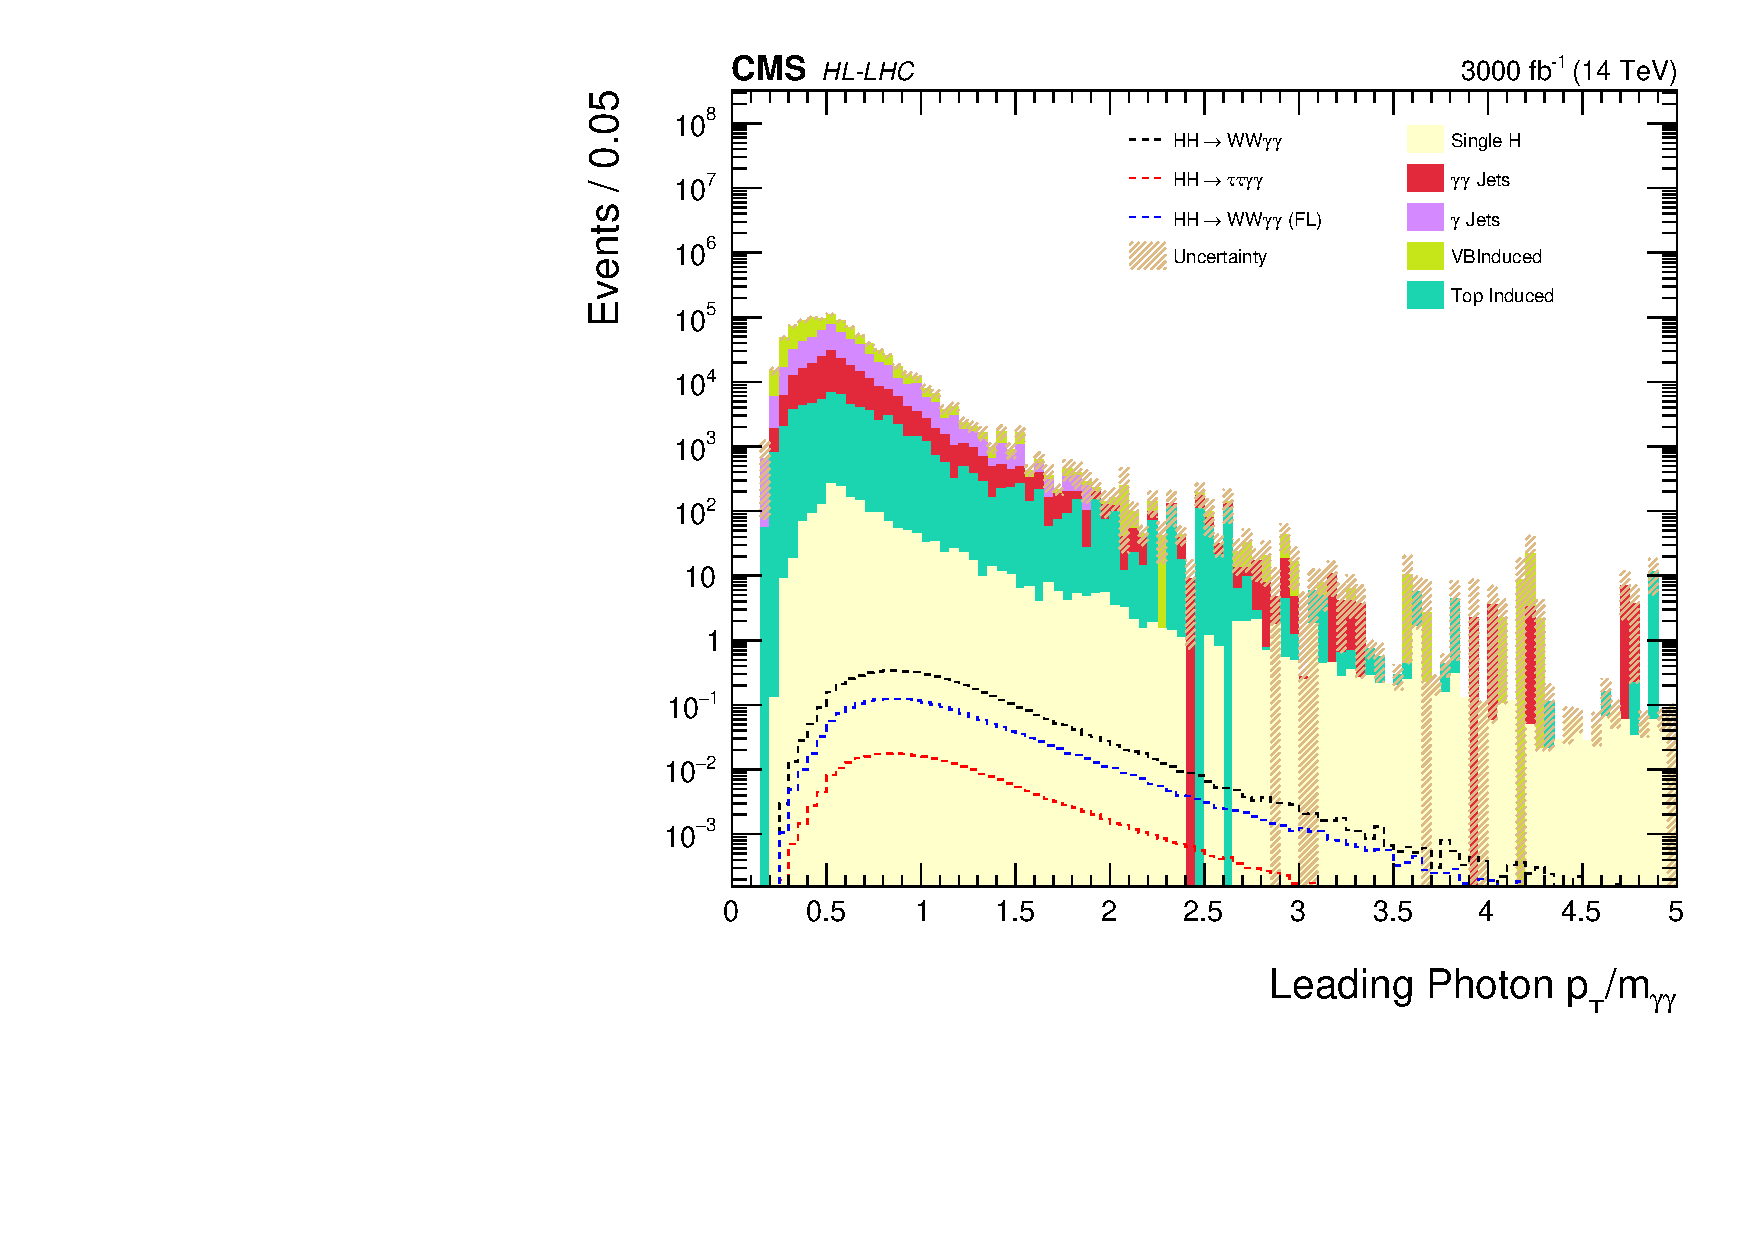
\includegraphics[width=\textwidth]{LeadingPhotonpT_mGGLhasOneL_logy.pdf}
        \vspace{-0.5cm}
        \firstsubcaption{Leading Photon p$_T$/\mgg}
    \end{subfigure}
    \hfill
    \begin{subfigure}[b]{0.475\textwidth}  
        \centering 
        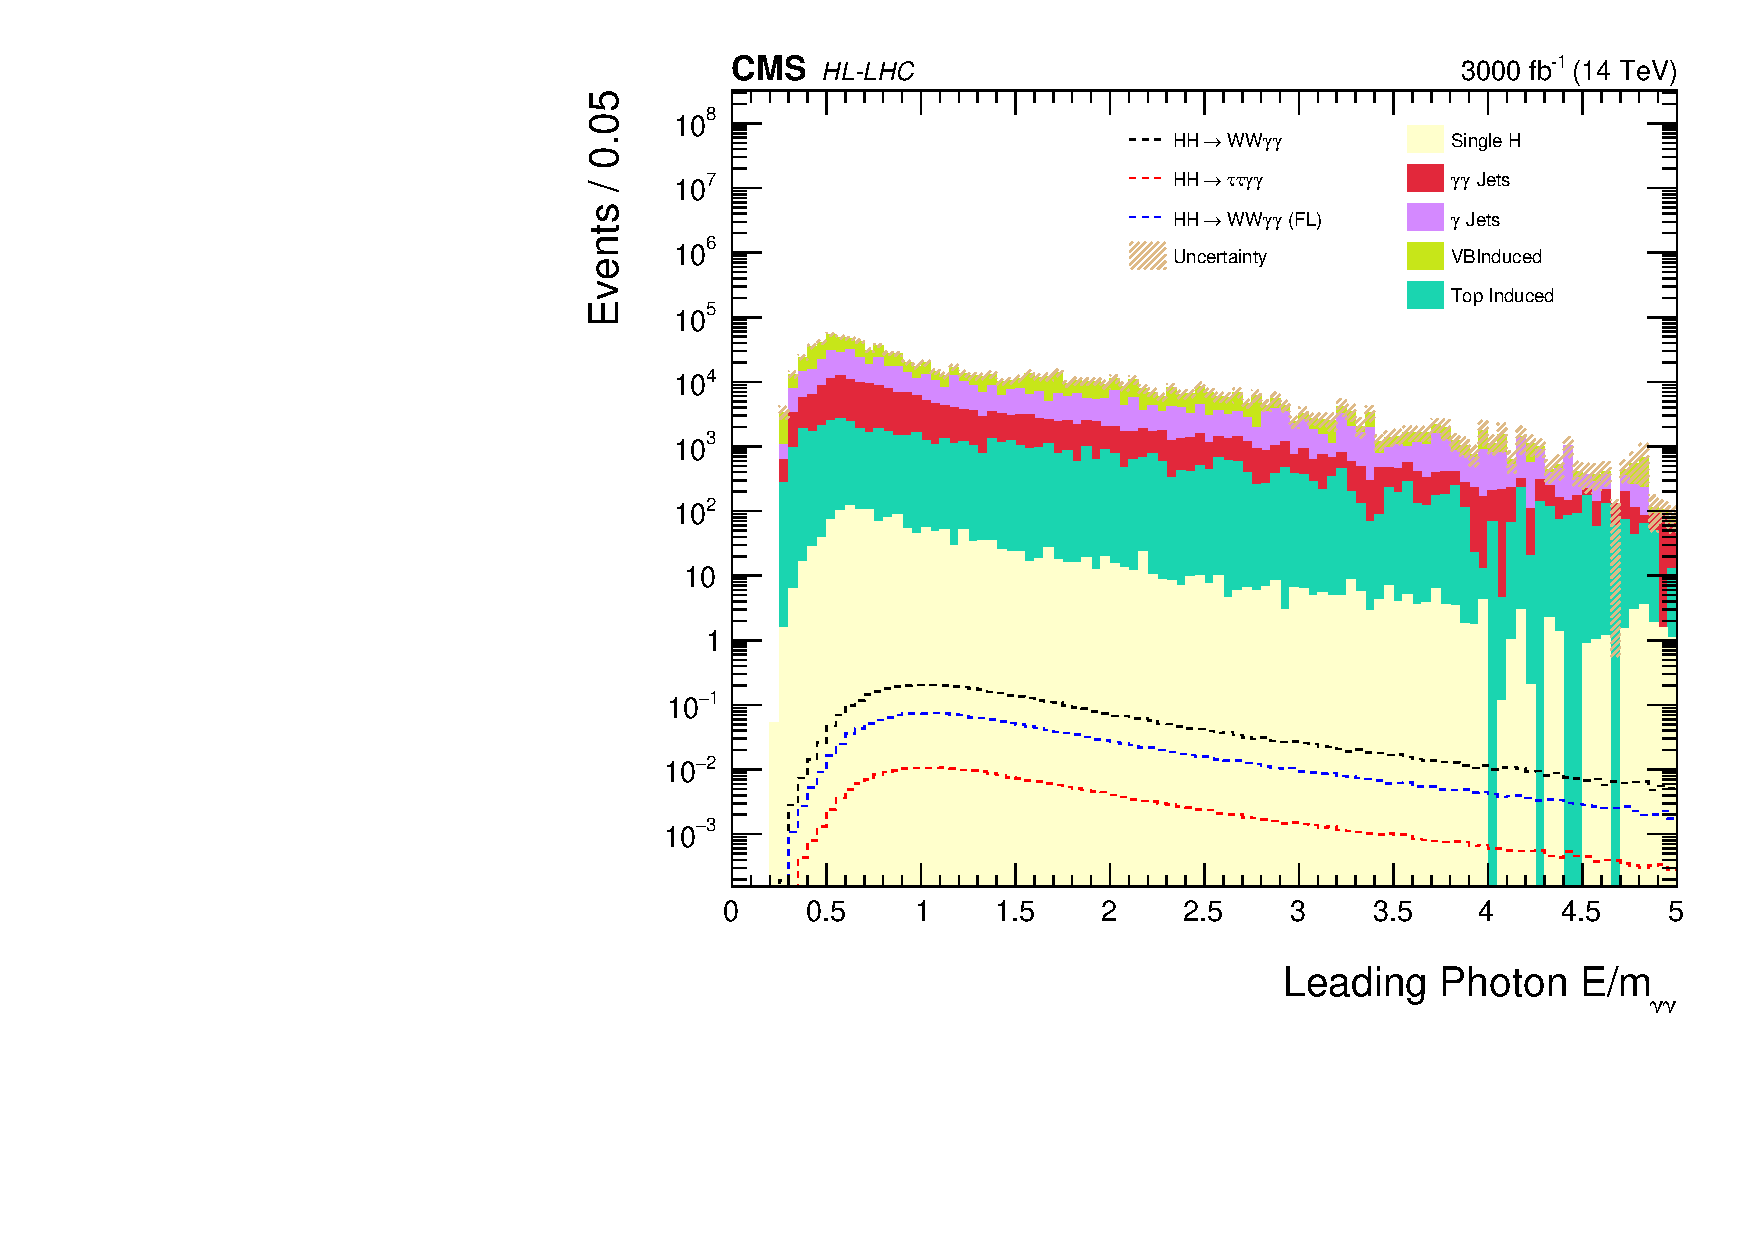
\includegraphics[width=\textwidth]{LeadingPhotonE_mGGLhasOneL_logy.pdf}
        \vspace{-0.5cm}
        \firstsubcaption{Leading Photon E/\mgg}
    \end{subfigure}
    \vskip\baselineskip
    \begin{subfigure}[b]{0.475\textwidth}   
        \centering 
        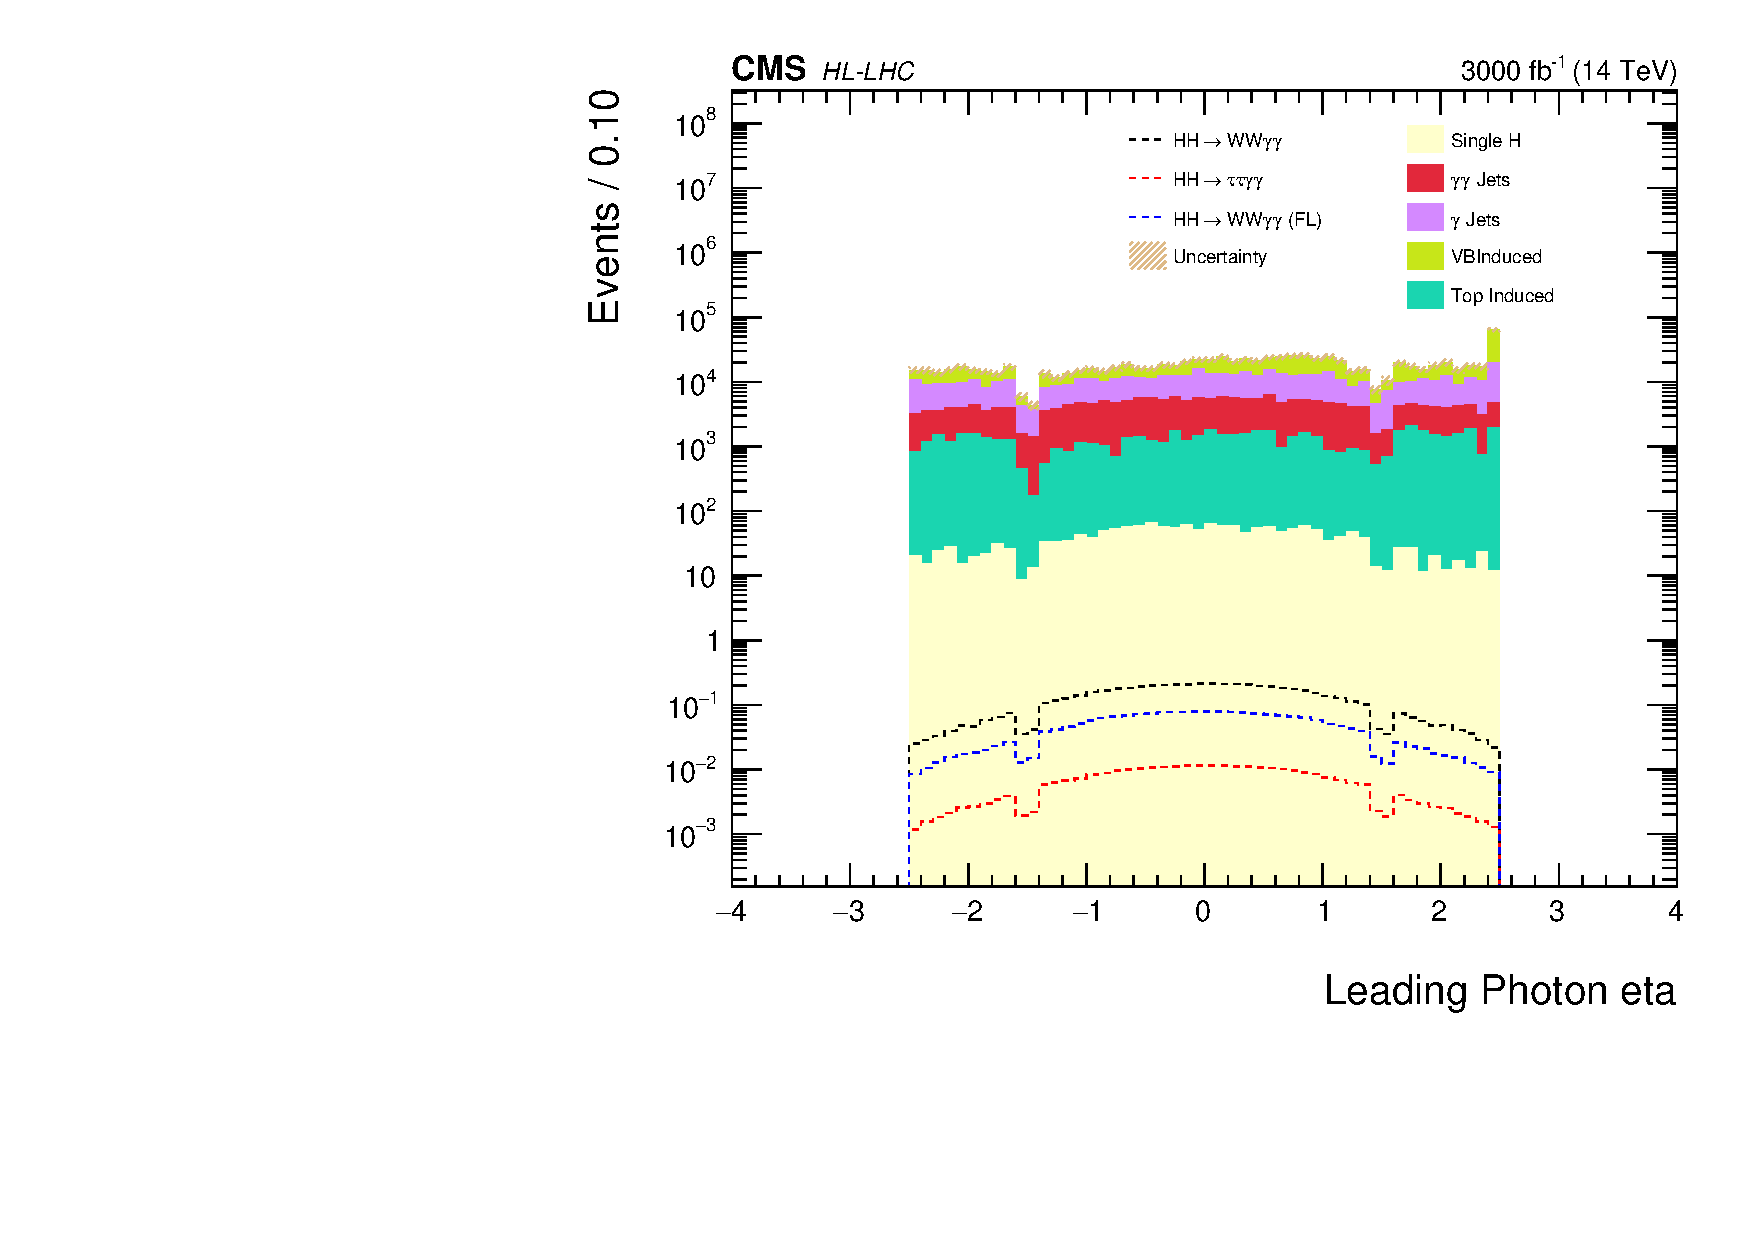
\includegraphics[width=\textwidth]{LeadingPhotonEtaOneL_logy.pdf}
        \vspace{-0.5cm}
        \firstsubcaption{Leading Photon $\eta$}
    \end{subfigure}
    \hfill
    \begin{subfigure}[b]{0.475\textwidth}   
        \centering 
        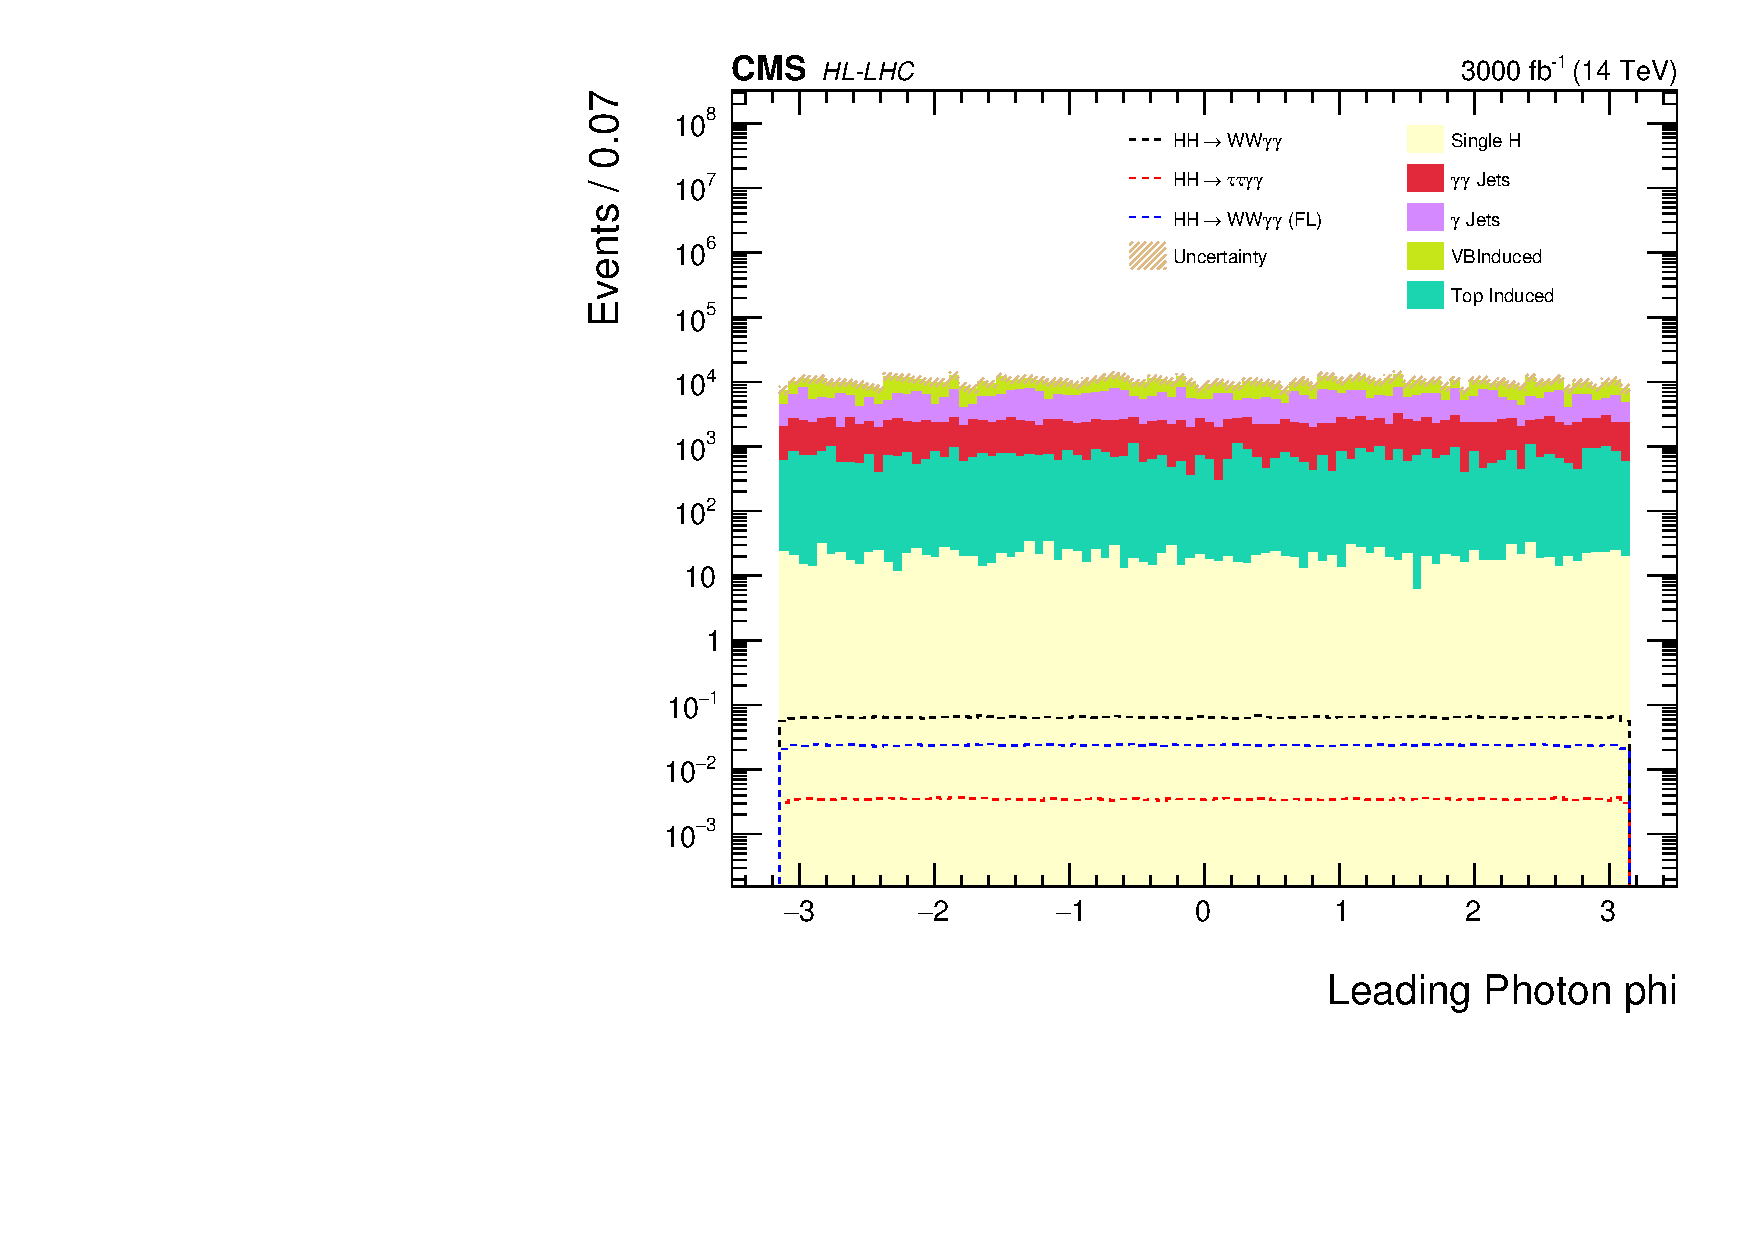
\includegraphics[width=\textwidth]{LeadingPhotonPhiOneL_logy.pdf}
        \vspace{-0.5cm}
        \firstsubcaption{Leading Photon $\phi$}
    \end{subfigure}
    \vskip\baselineskip
    \begin{subfigure}[b]{0.475\textwidth}   
        \centering 
        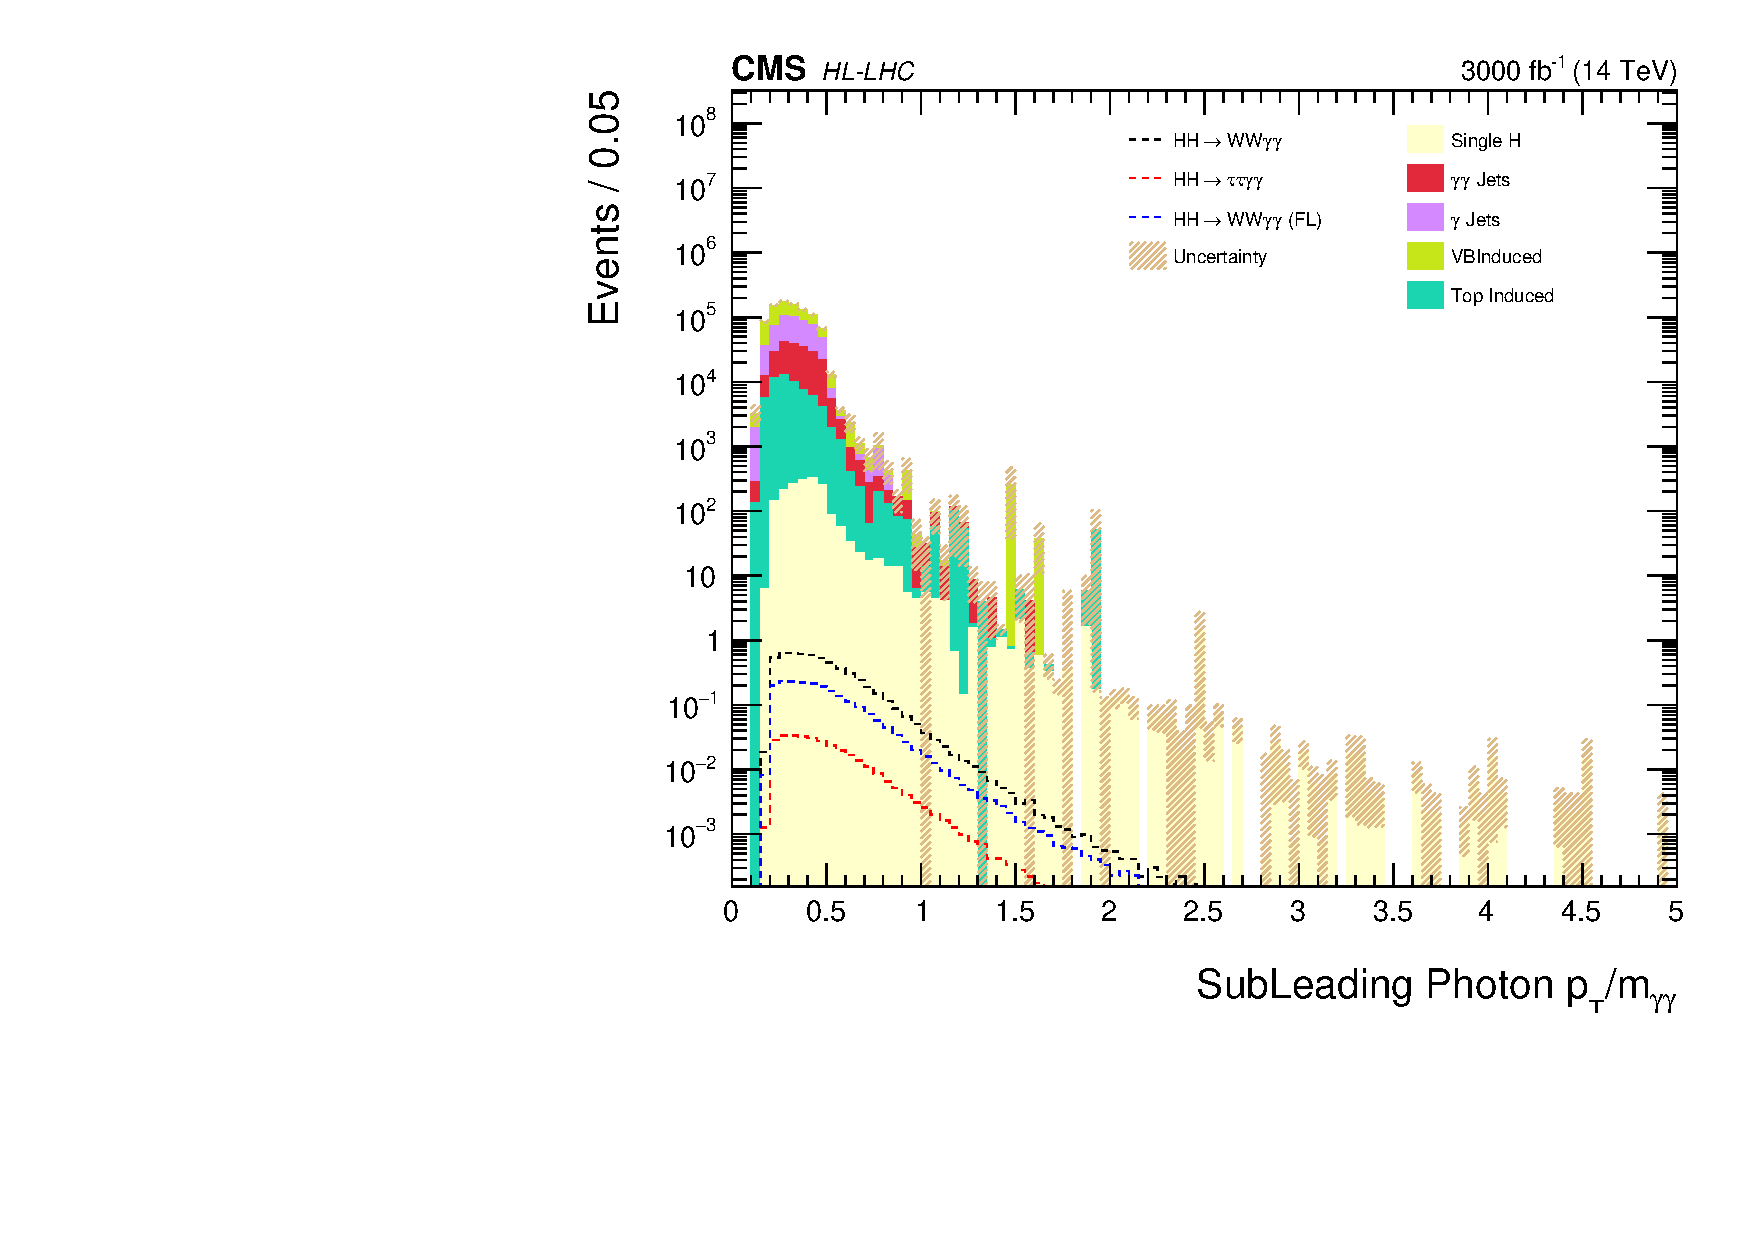
\includegraphics[width=\textwidth]{SubLeadingPhotonpT_mGGLhasOneL_logy.pdf}
        \vspace{-0.5cm}
        \firstsubcaption{Sub-leading Photon p$_T$/\mgg}
    \end{subfigure}
    \hfill
    \begin{subfigure}[b]{0.475\textwidth}   
        \centering 
        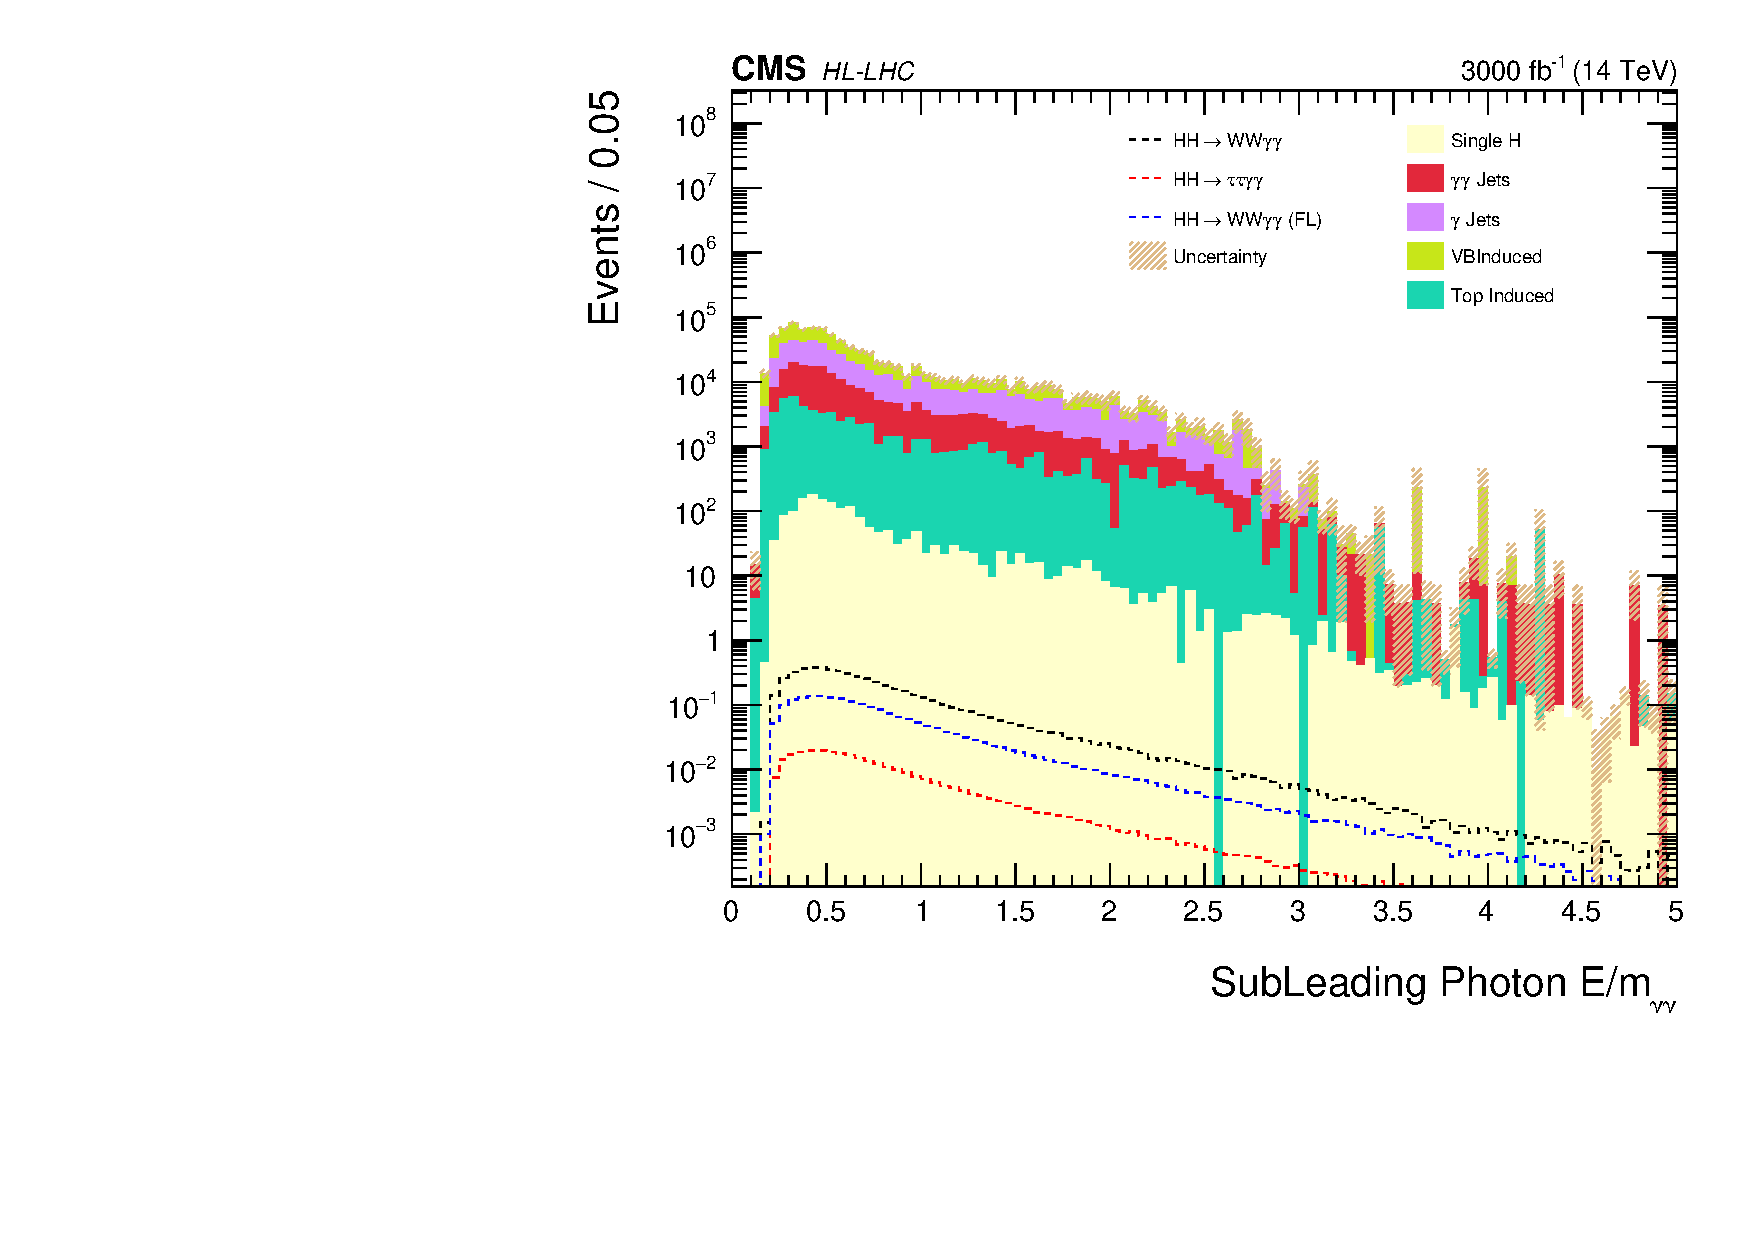
\includegraphics[width=\textwidth]{SubLeadingPhotonE_mGGLhasOneL_logy.pdf}
        \vspace{-0.5cm}
        \firstsubcaption{Sub-leading Photon E/\mgg}   
    \end{subfigure}
    \caption{\small DNN input distributions for the semi-leptonic channel of $HH\rightarrow{WW\gamma\gamma}$.} 
    \label{hasOneL_plots}
\end{figure*}

\begin{figure*}[h!]
    \centering
    \begin{subfigure}[b]{0.475\textwidth}
        \centering
        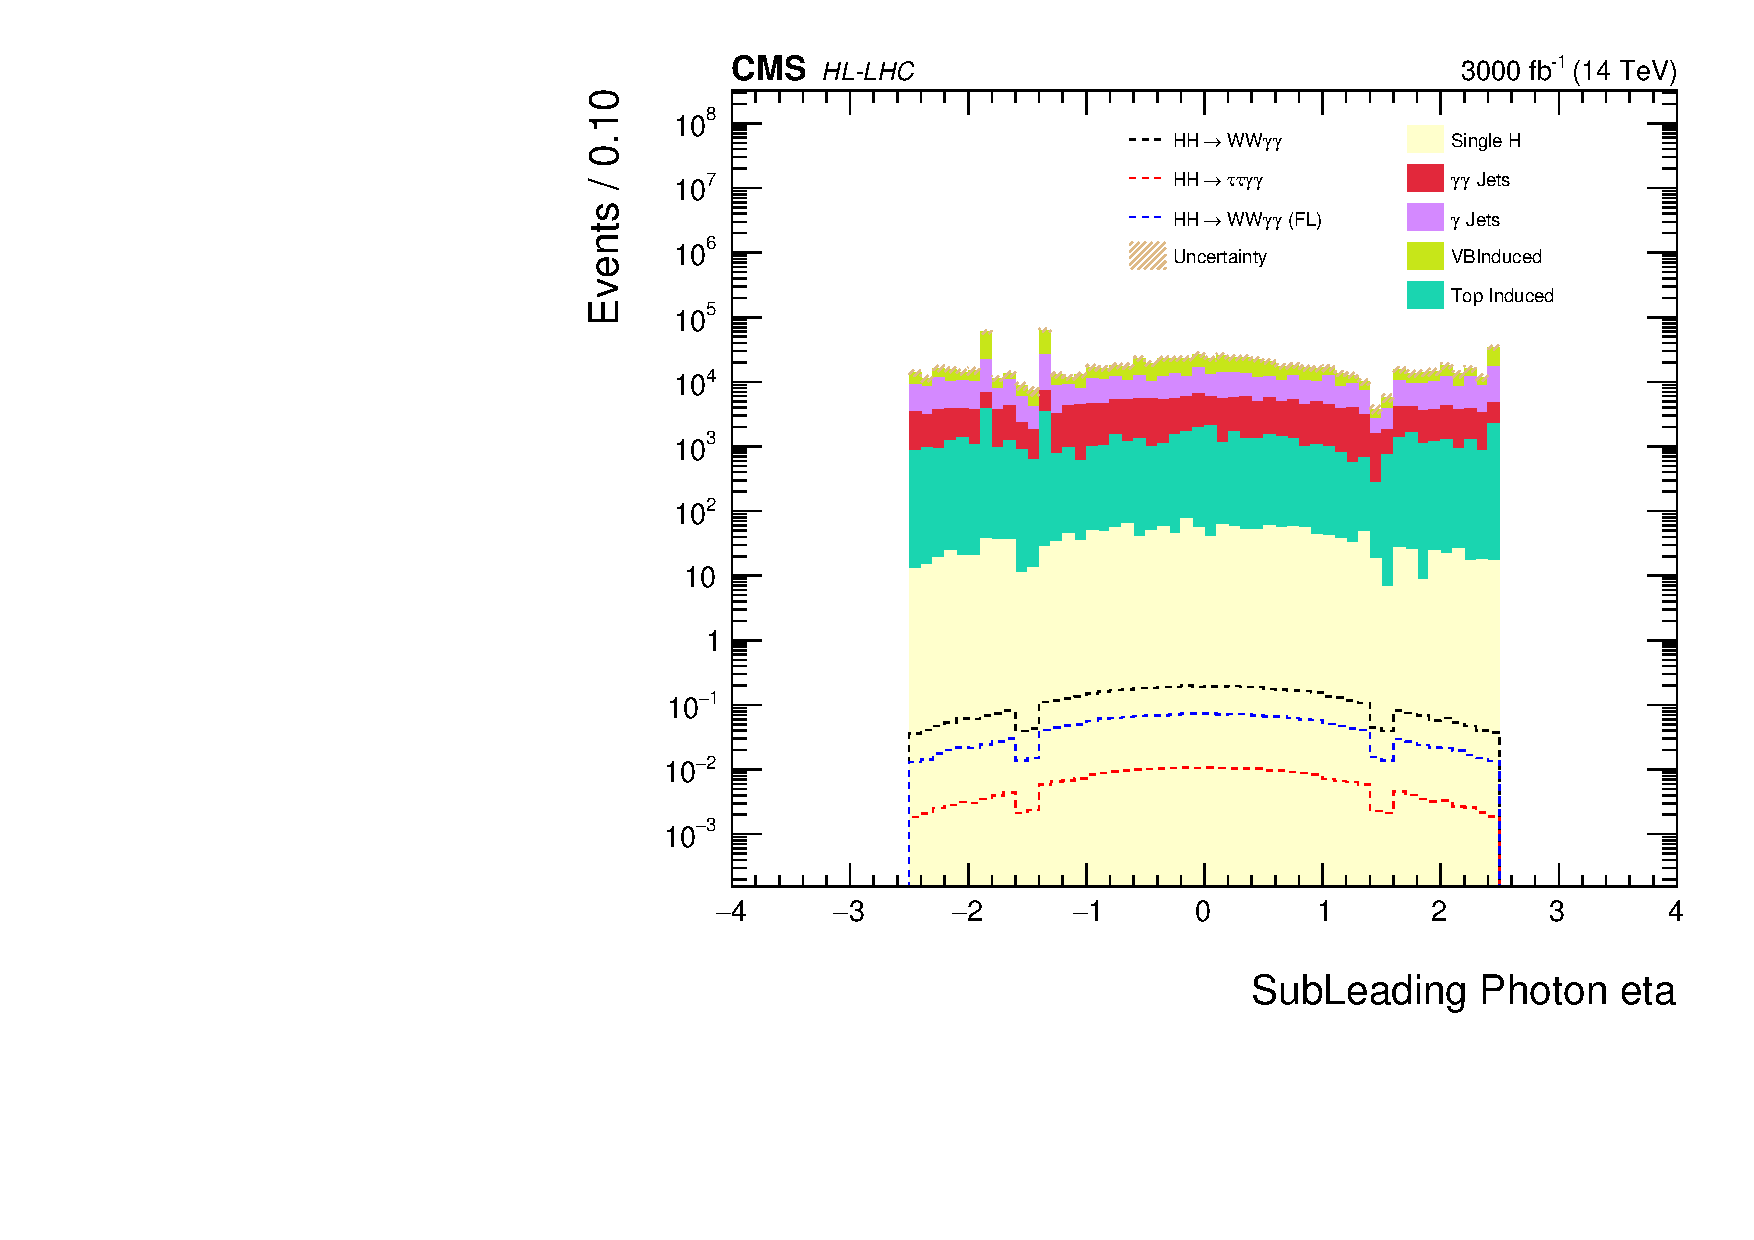
\includegraphics[width=\textwidth]{SubLeadingPhotonEtaOneL_logy.pdf}
        \vspace{-0.5cm}
        \firstsubcaption{Sub-leading Photon $\eta$}
    \end{subfigure}
    \hfill
    \begin{subfigure}[b]{0.475\textwidth}  
        \centering 
        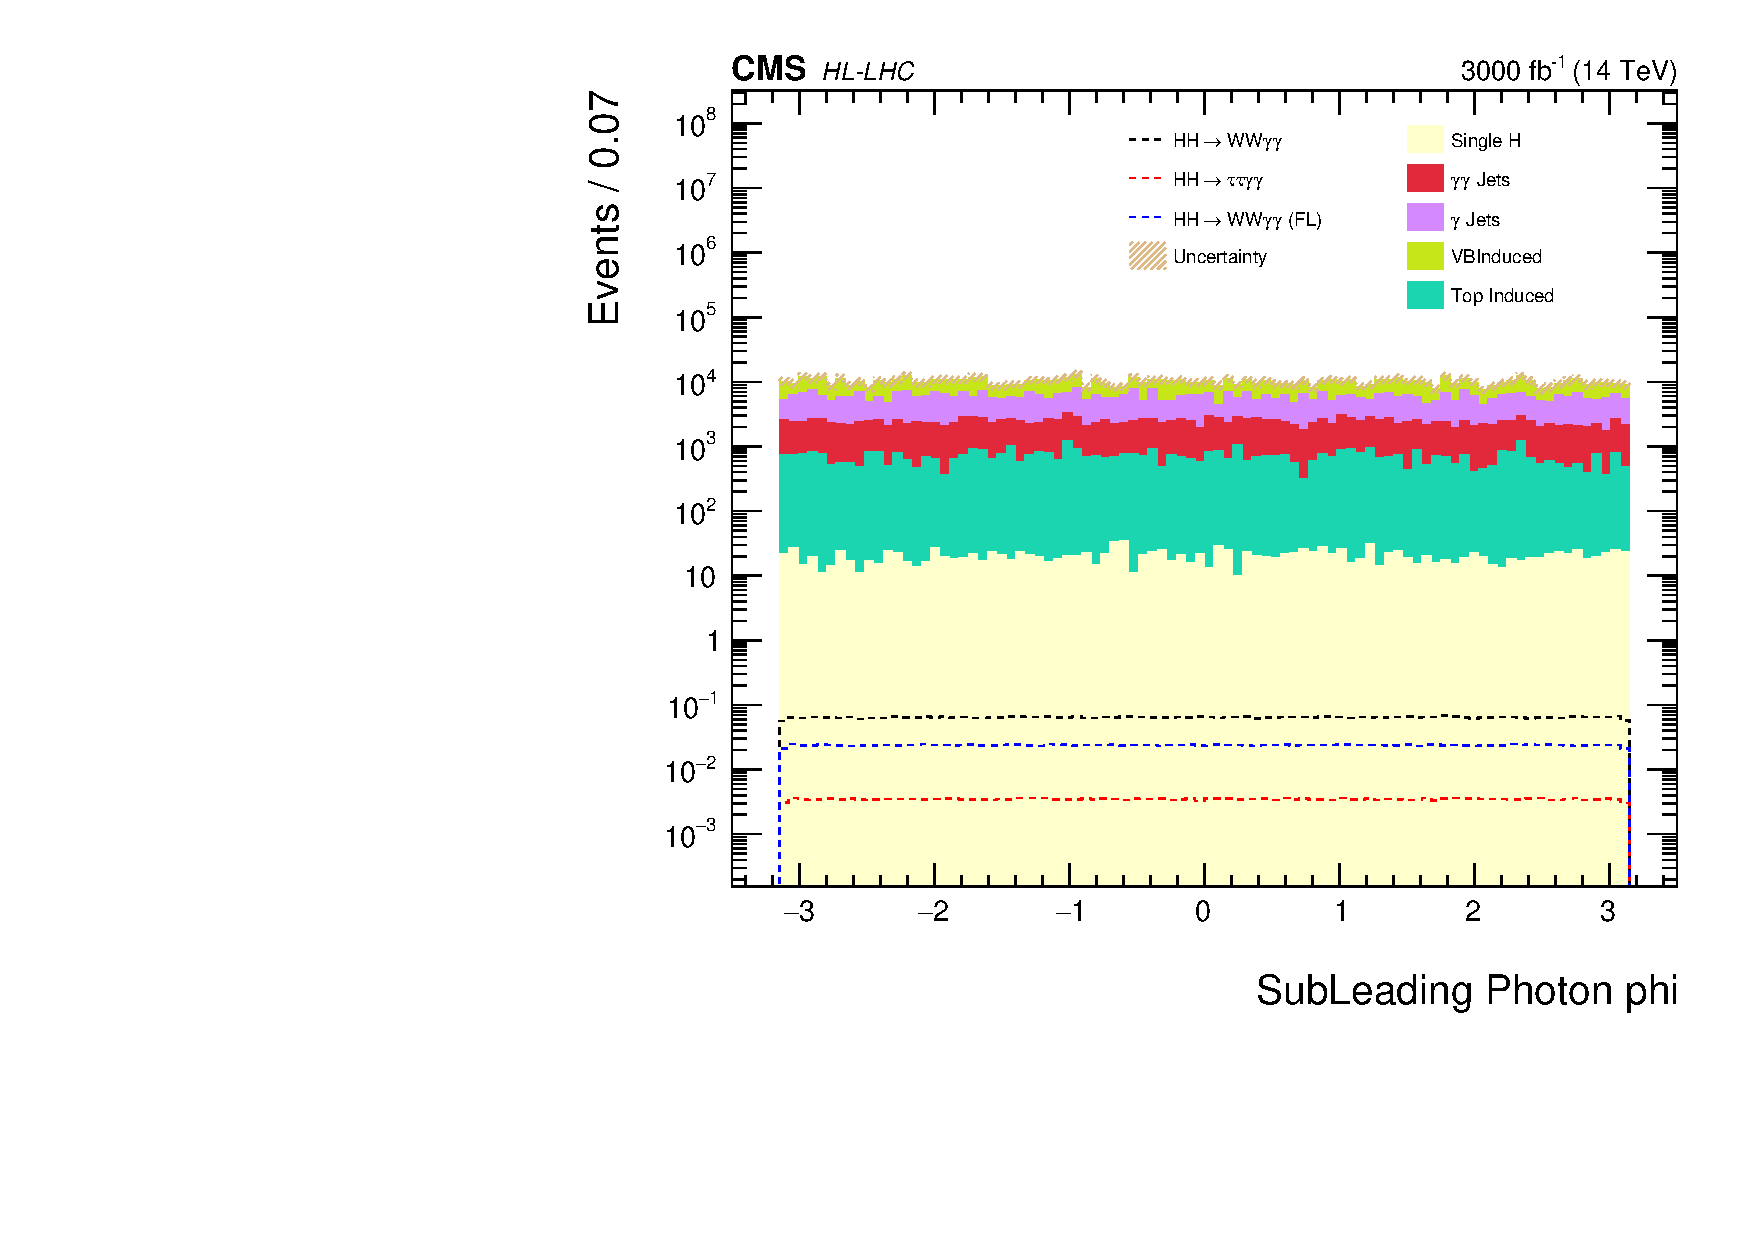
\includegraphics[width=\textwidth]{SubLeadingPhotonPhiOneL_logy.pdf}
        \vspace{-0.5cm}
        \firstsubcaption{Sub-leading Photon $\phi$}
    \end{subfigure}
    \vskip\baselineskip
    \begin{subfigure}[b]{0.475\textwidth}   
        \centering 
        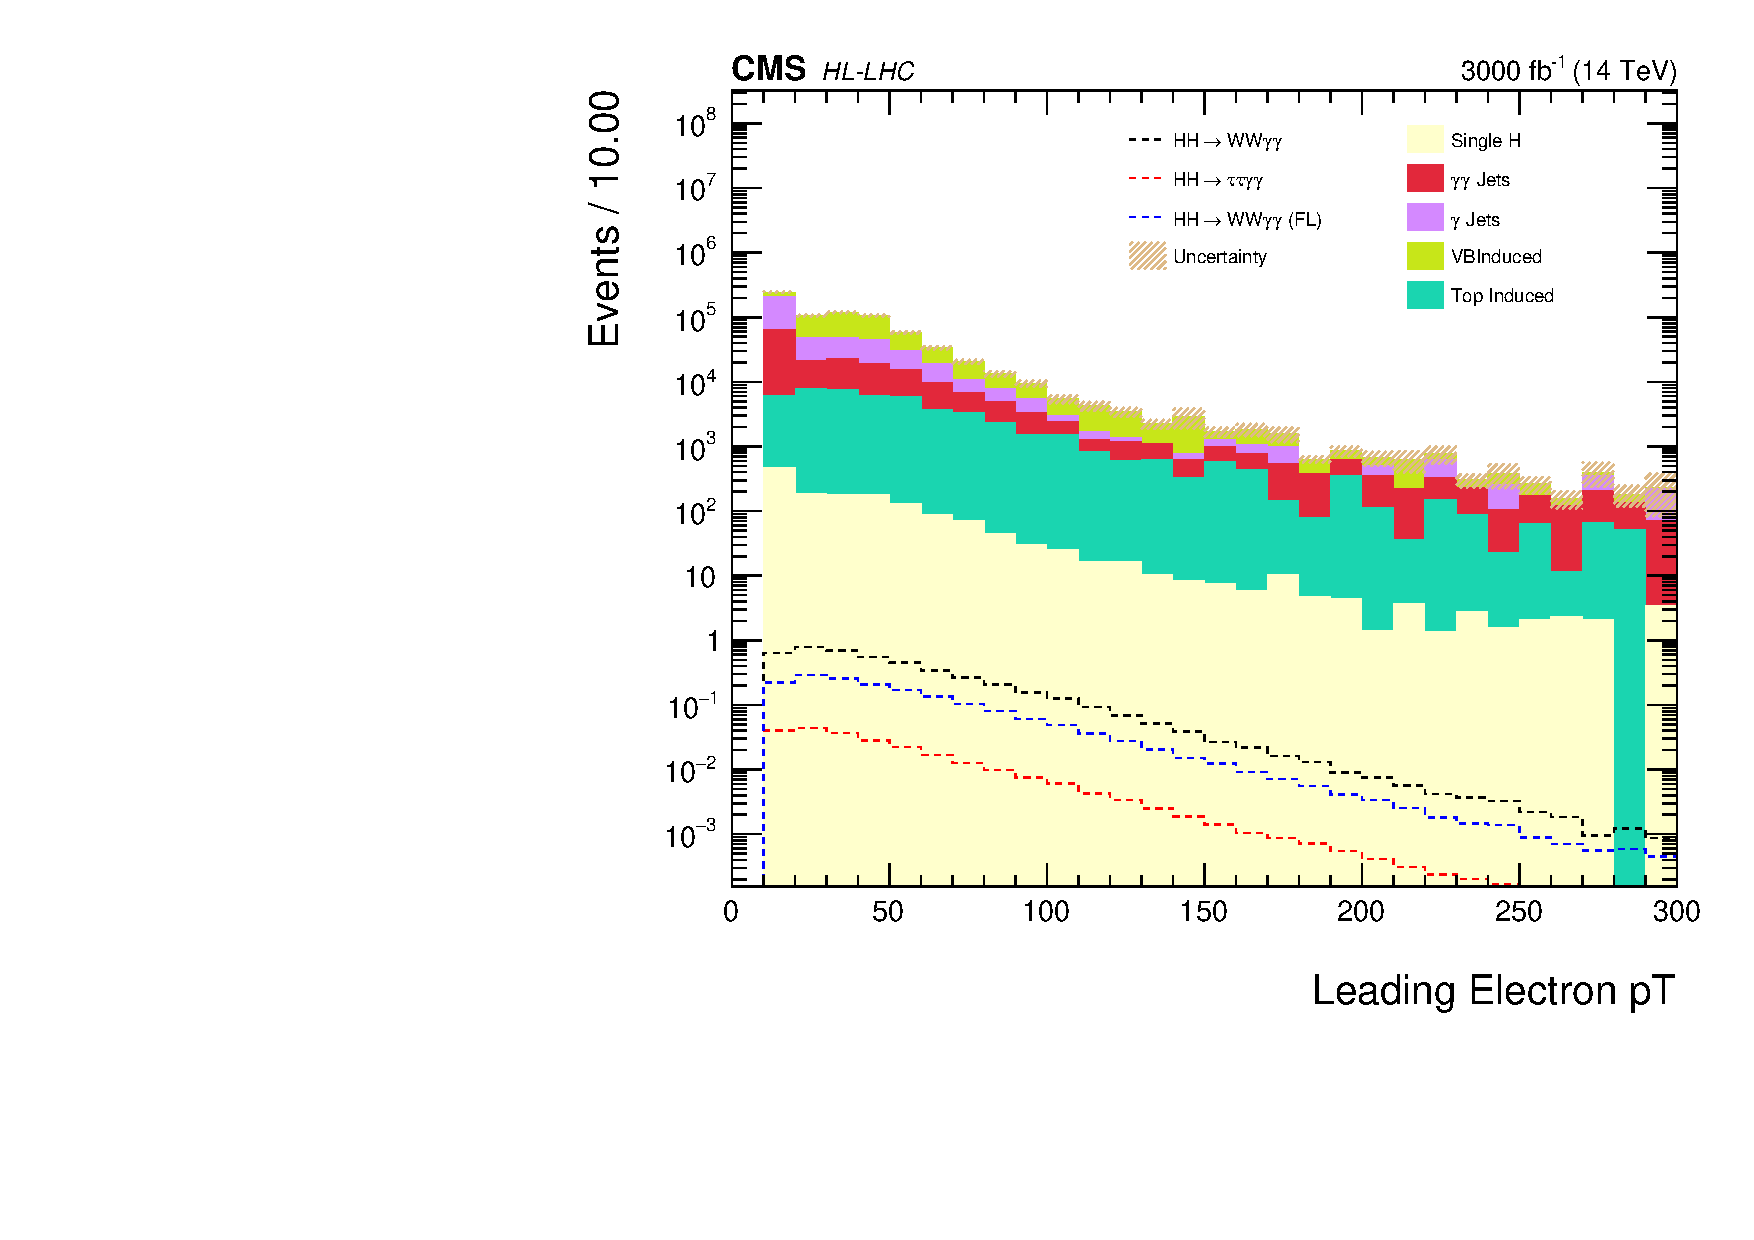
\includegraphics[width=\textwidth]{ElectronpT_logy.pdf}
        \vspace{-0.5cm}
        \firstsubcaption{Leading Electron p$_{T}$}
    \end{subfigure}
    \hfill
    \begin{subfigure}[b]{0.475\textwidth}   
        \centering 
        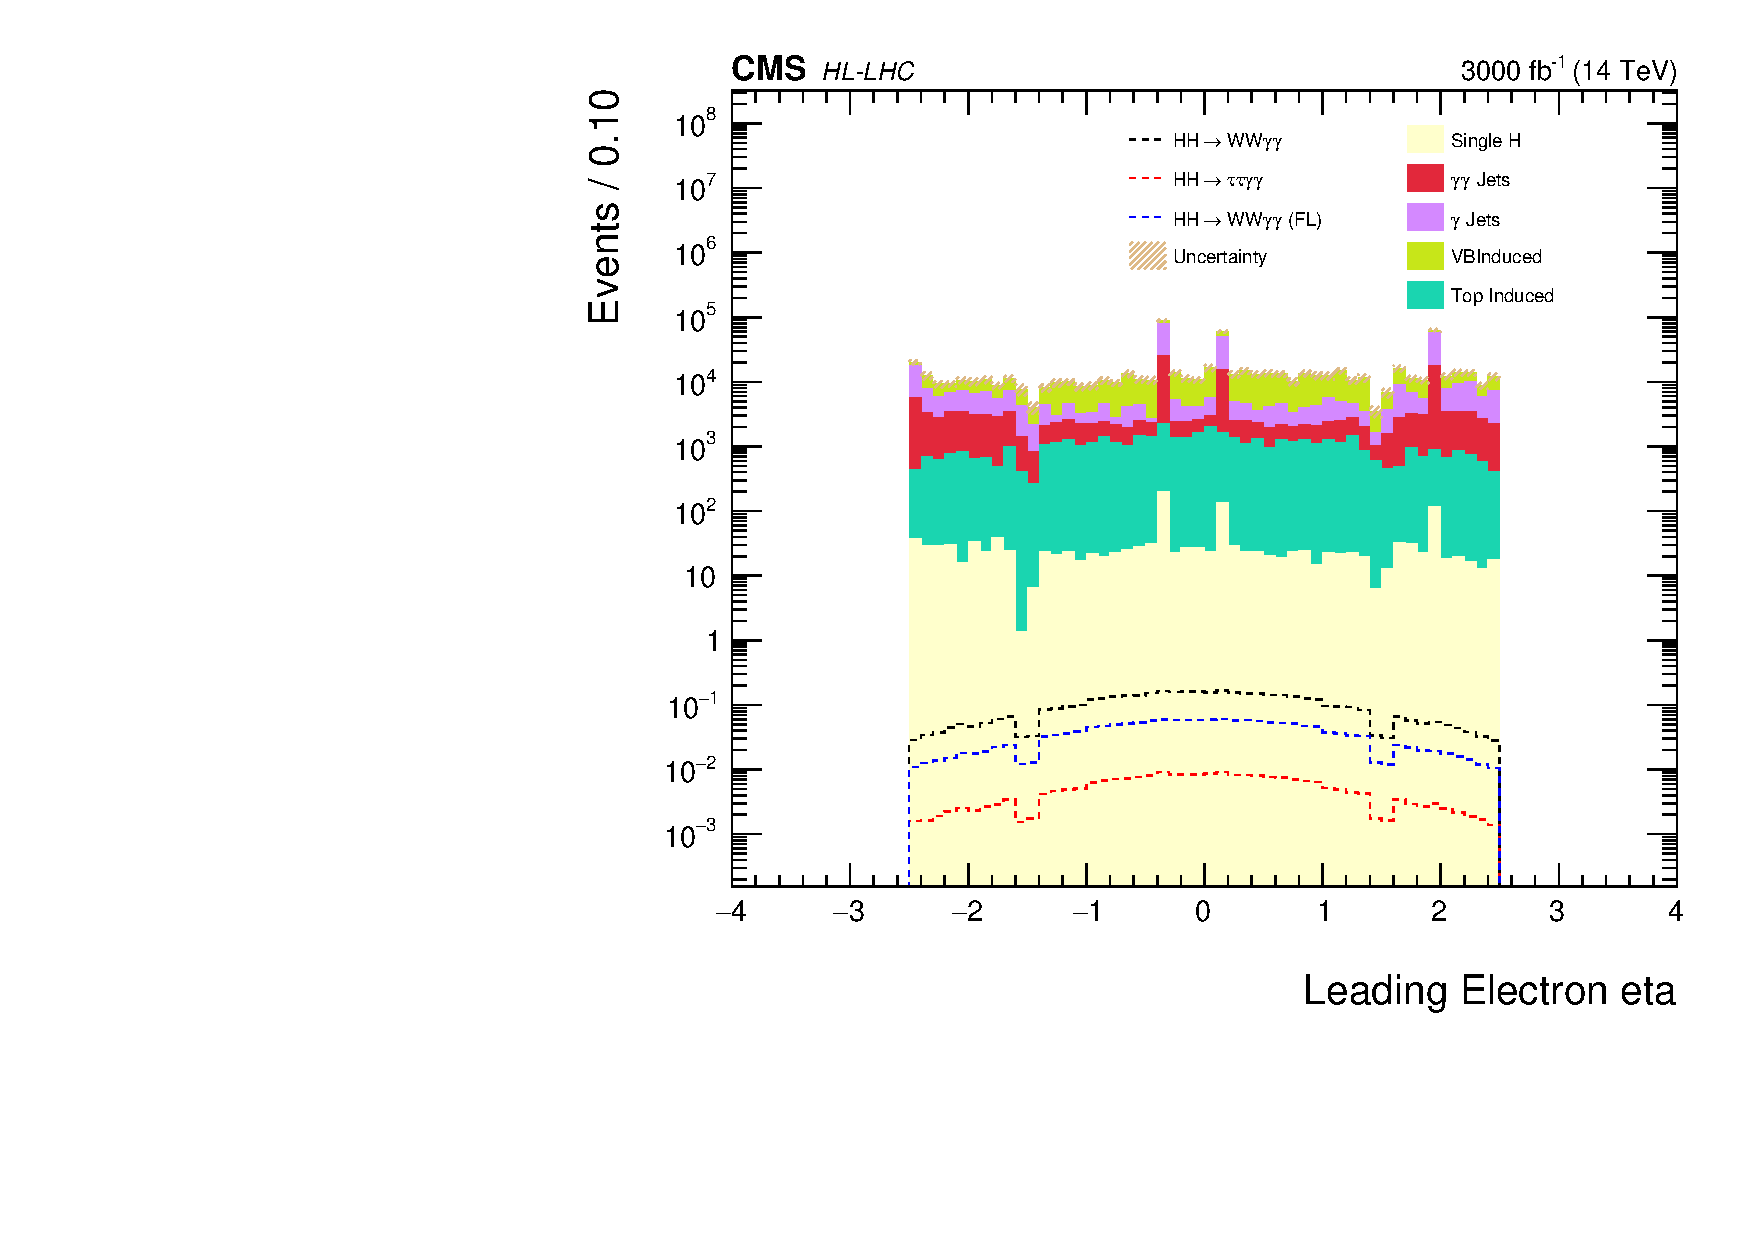
\includegraphics[width=\textwidth]{ElectronEta_logy.pdf}
        \vspace{-0.5cm}
        \firstsubcaption{Leading Electron $\eta$}
    \end{subfigure}
    \vskip\baselineskip
    \begin{subfigure}[b]{0.475\textwidth}   
        \centering 
        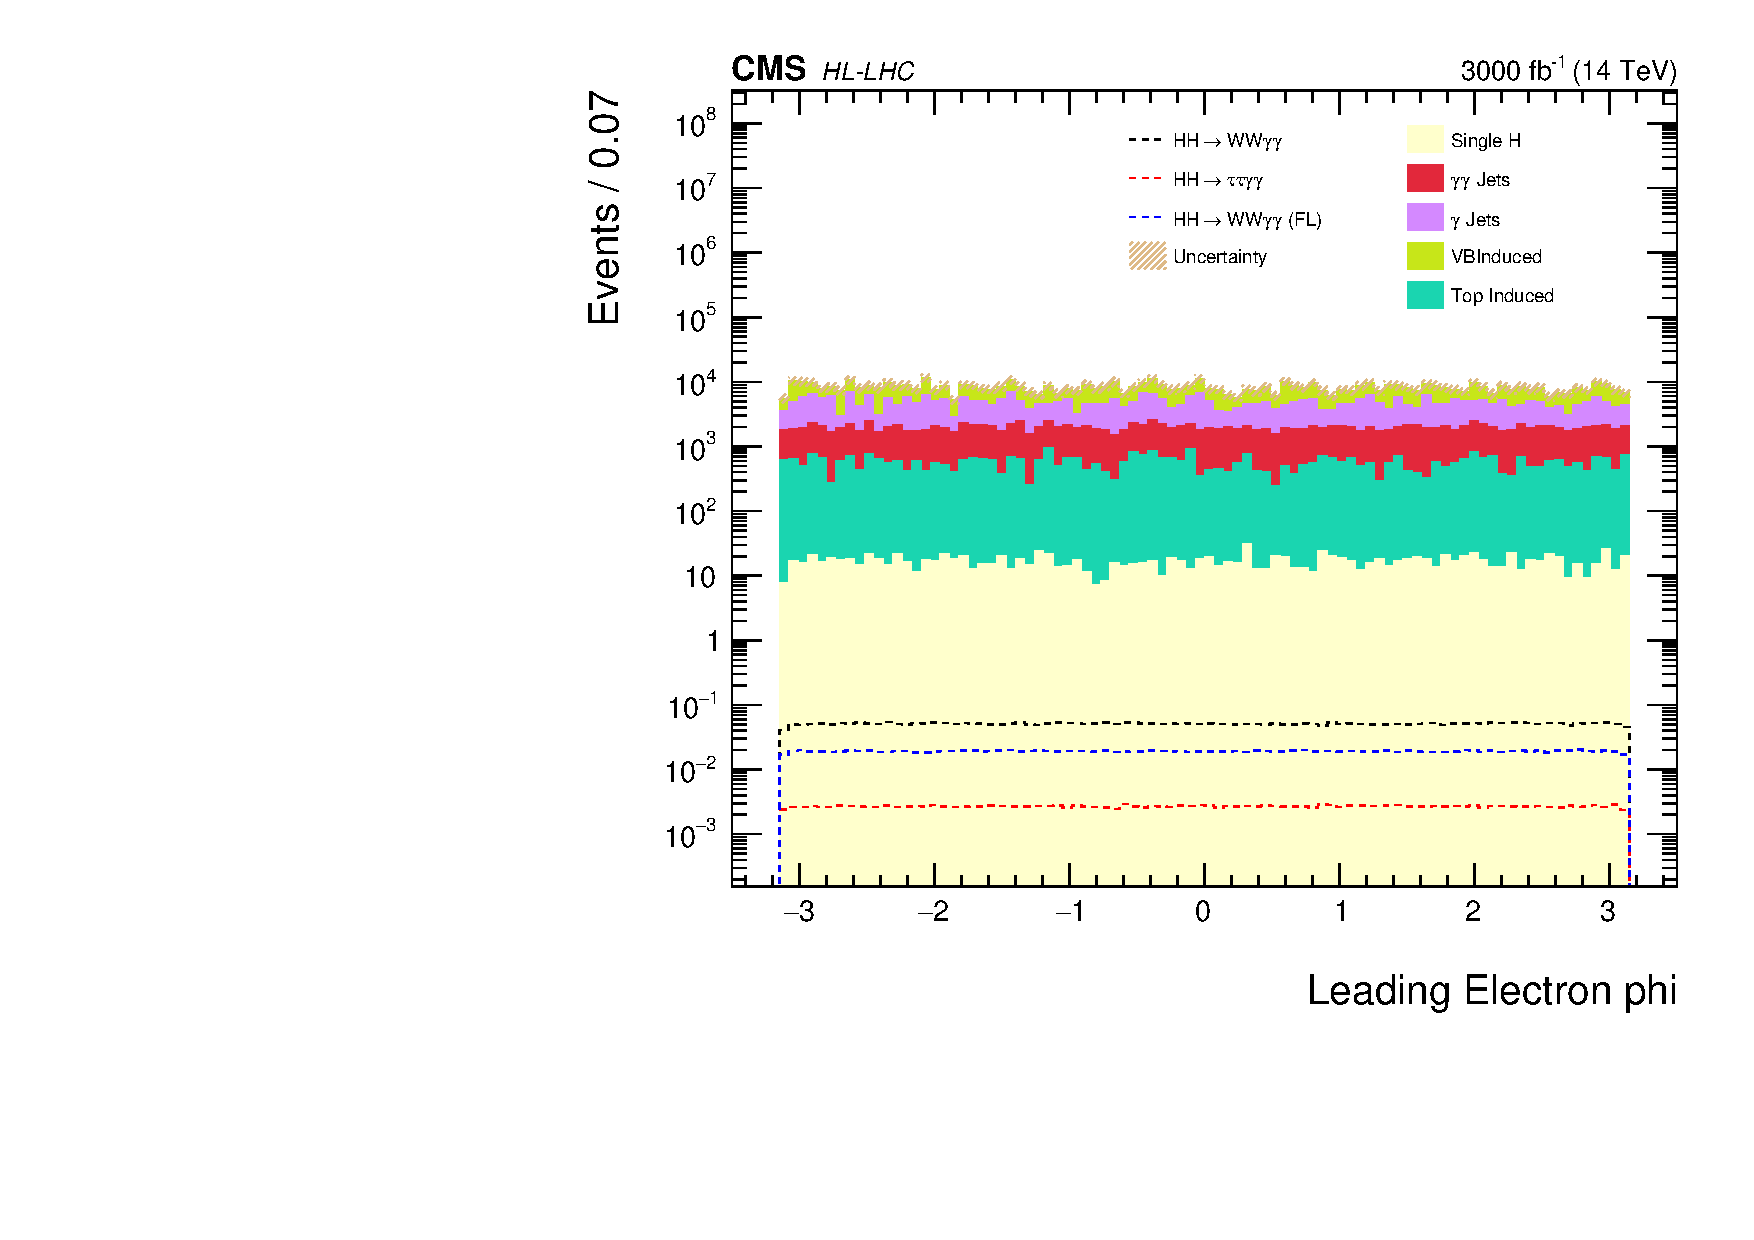
\includegraphics[width=\textwidth]{ElectronPhi_logy.pdf}
        \vspace{-0.5cm}
        \firstsubcaption{Leading Electron $\phi$}
    \end{subfigure}
    \hfill
    \begin{subfigure}[b]{0.475\textwidth}   
        \centering 
        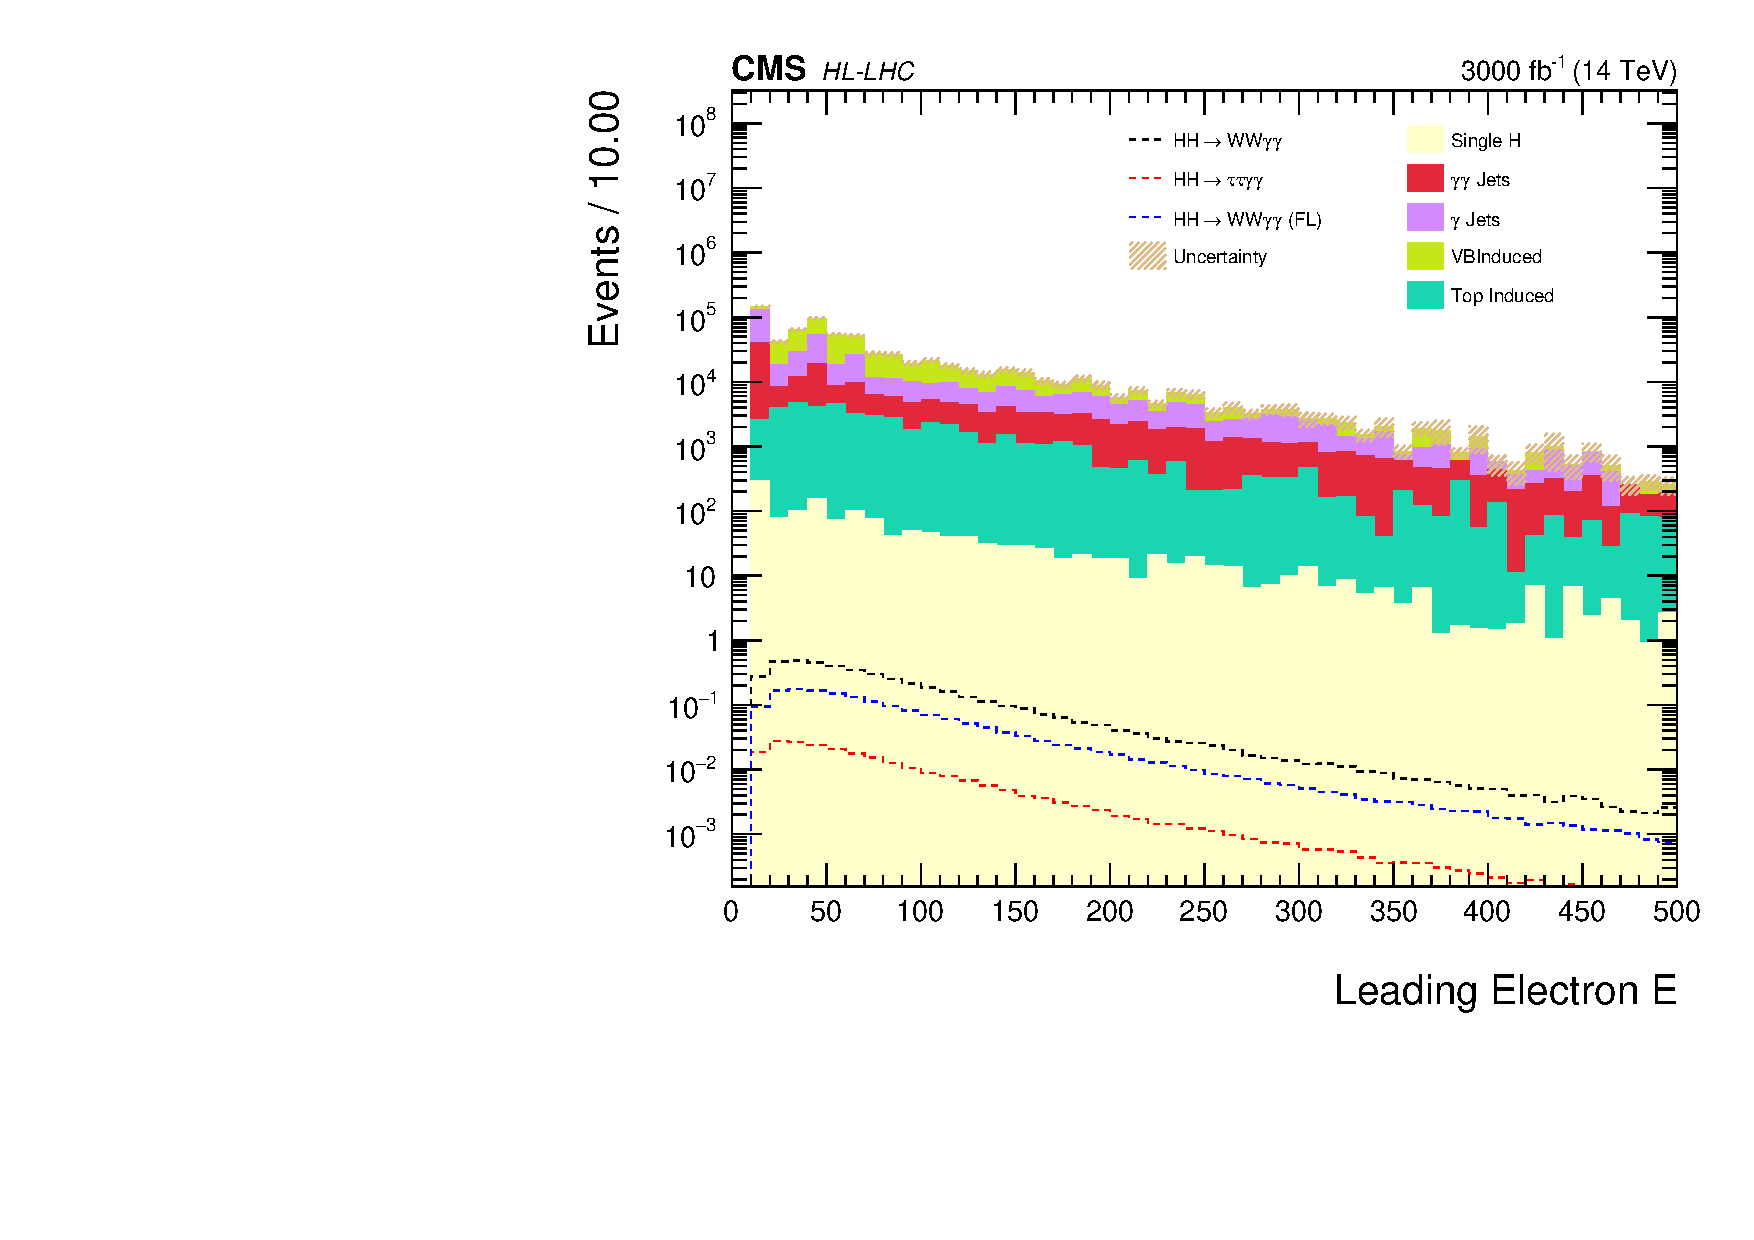
\includegraphics[width=\textwidth]{ElectronE_logy.pdf}
        \vspace{-0.5cm}
        \firstsubcaption{Leading Electron energy}   
    \end{subfigure}
    \caption{\small DNN input distributions for the semi-leptonic channel of $HH\rightarrow{WW\gamma\gamma}$ (continued).}
\end{figure*}

\begin{figure*}[h!]
    \centering
    \begin{subfigure}[b]{0.475\textwidth}
        \centering
        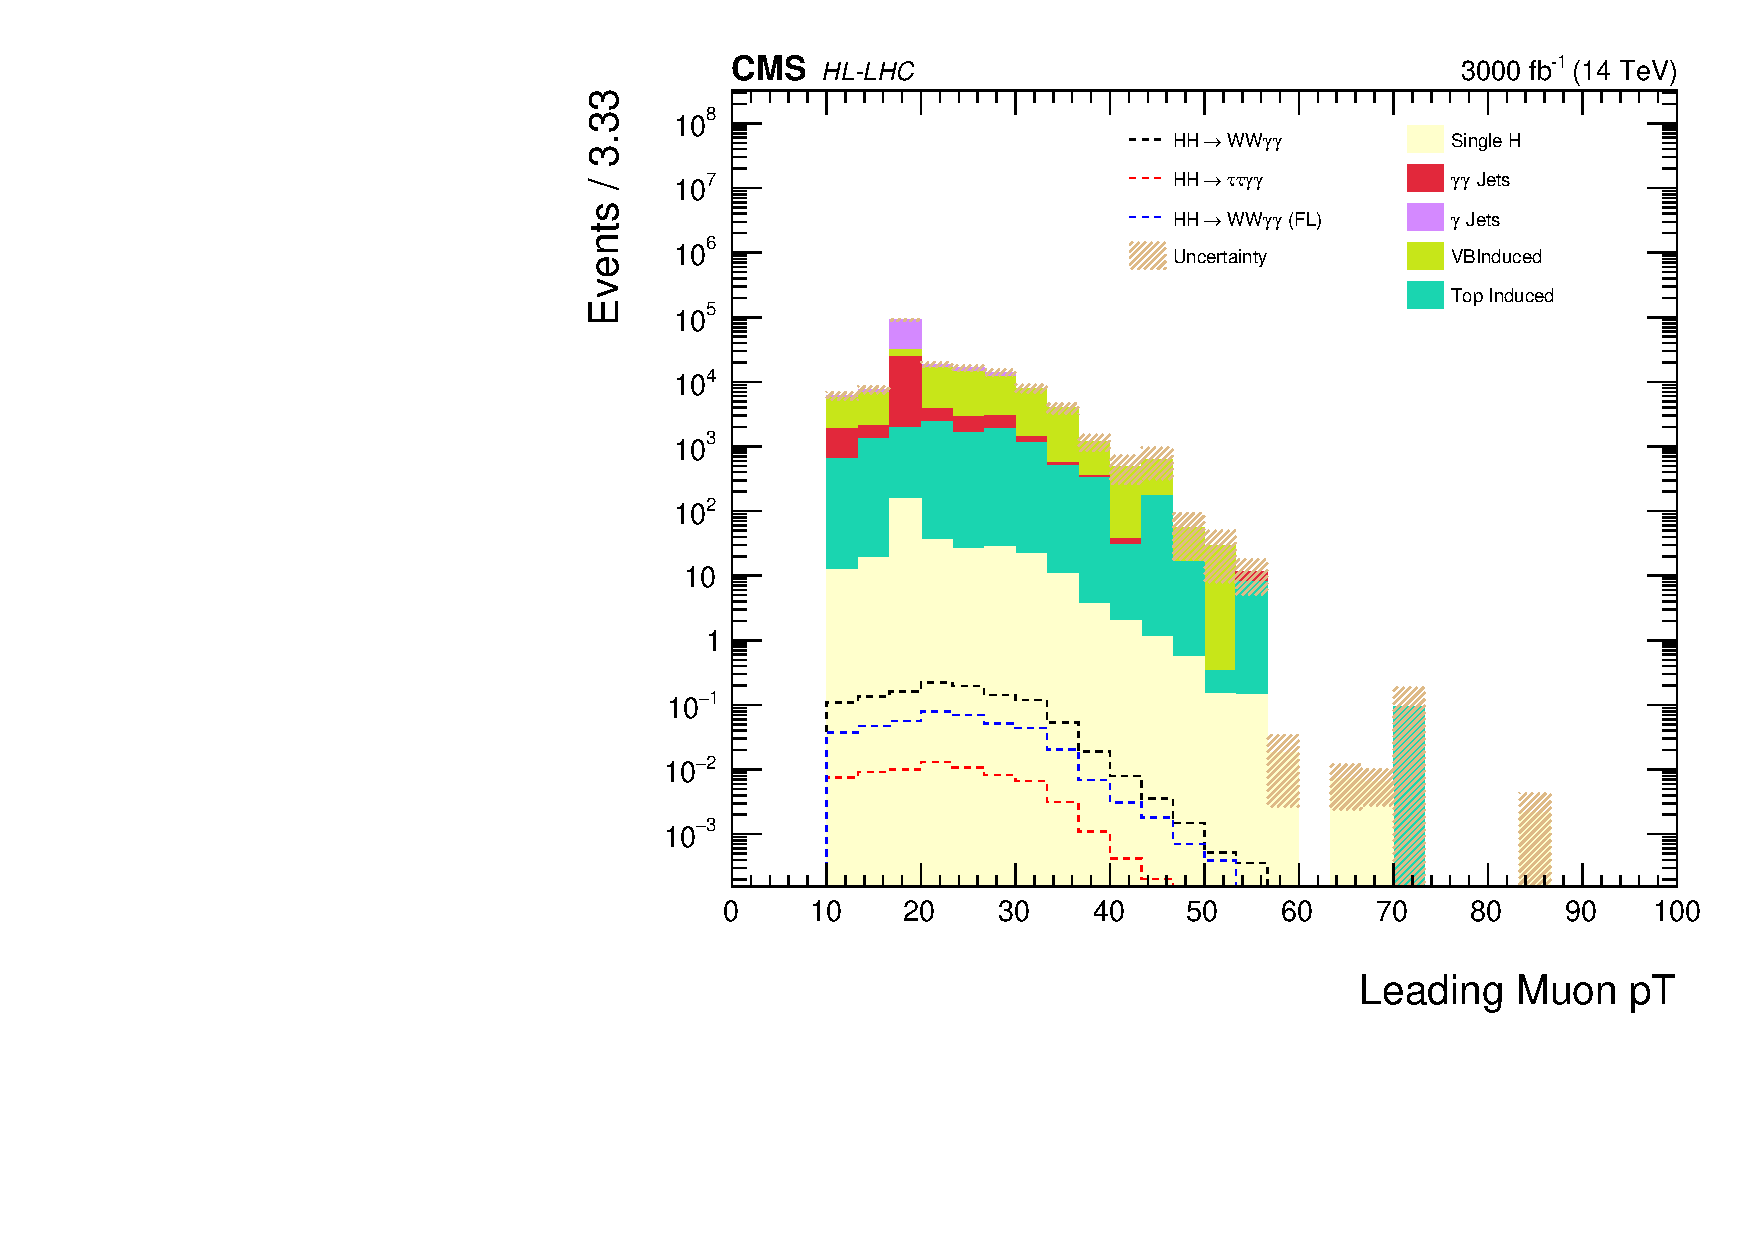
\includegraphics[width=\textwidth]{MuonpT_logy.pdf}
        \vspace{-0.5cm}
        \firstsubcaption{Leading Muon \pt}
    \end{subfigure}
    \hfill
    \begin{subfigure}[b]{0.475\textwidth}  
        \centering 
        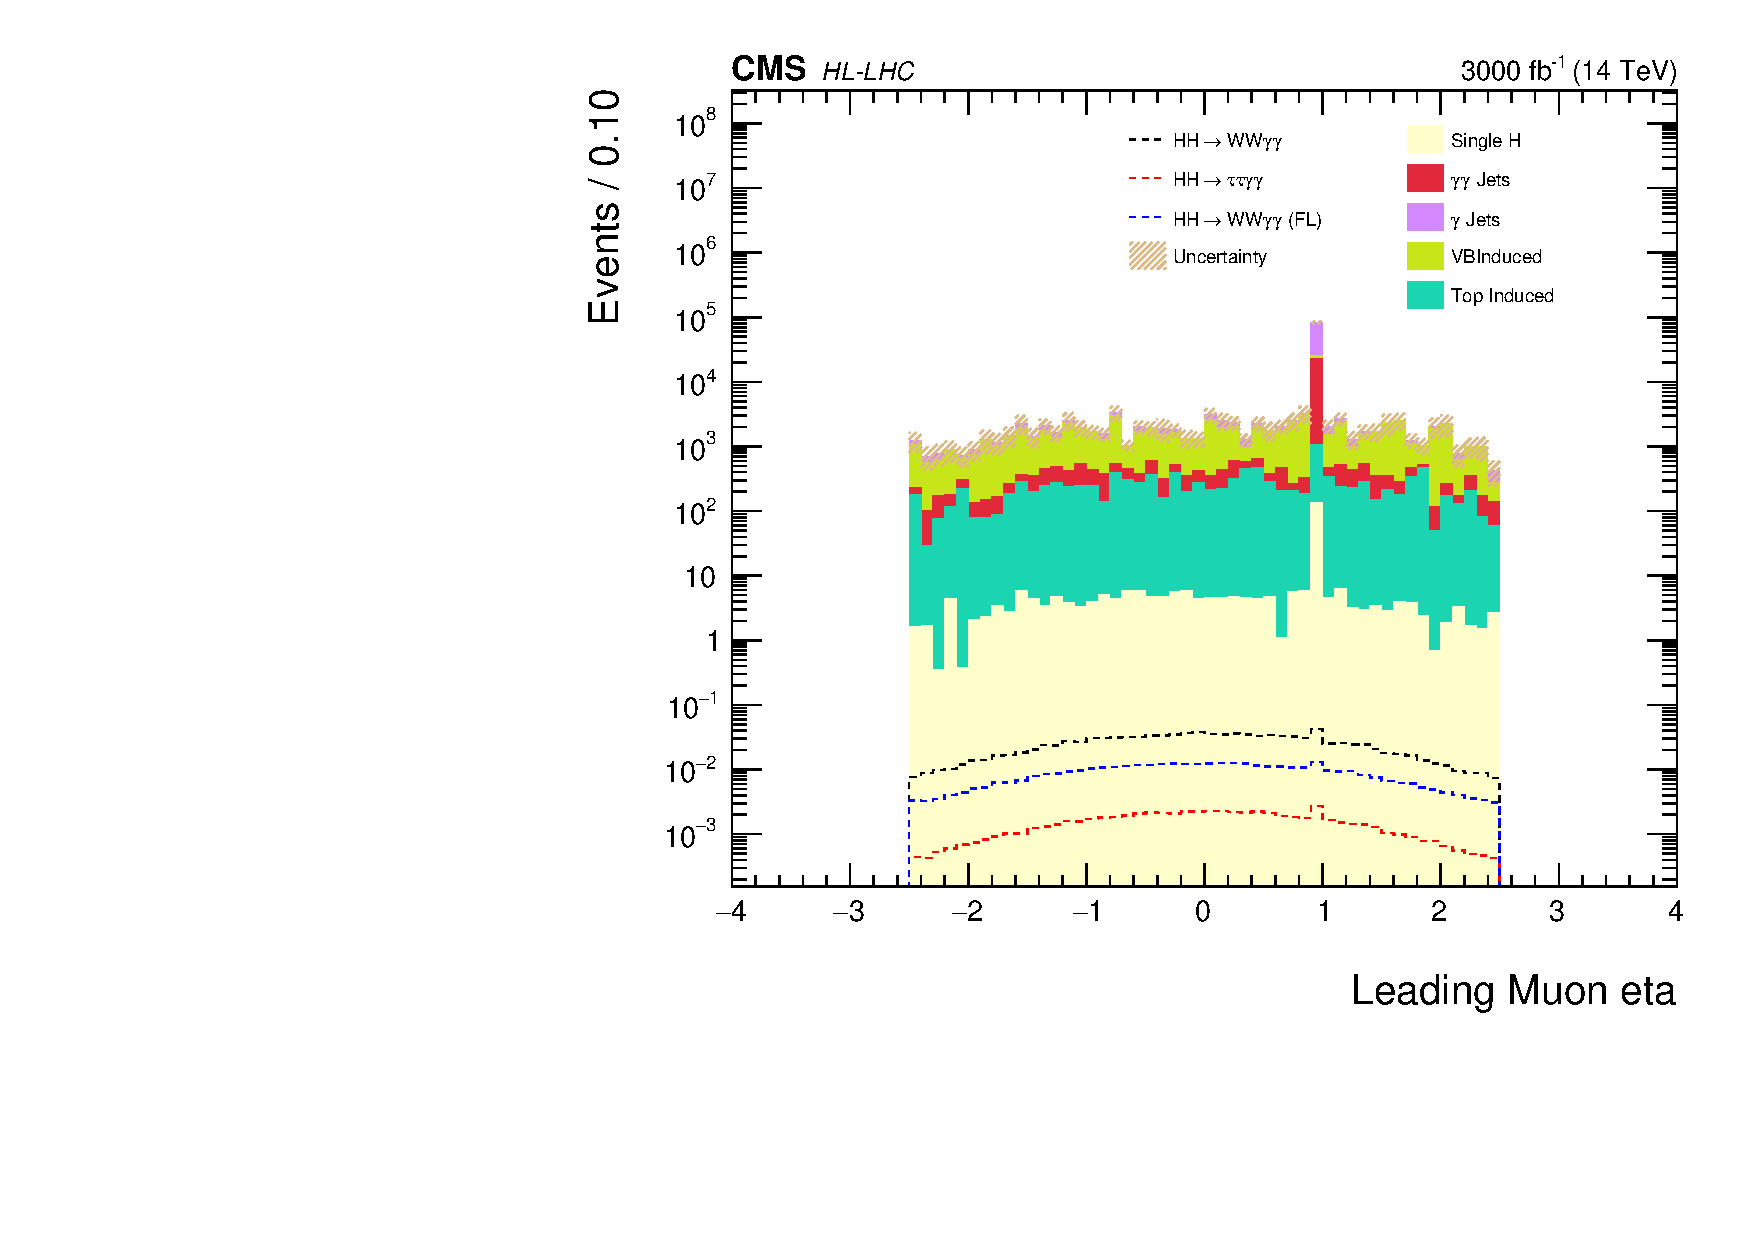
\includegraphics[width=\textwidth]{MuonEta_logy.pdf}
        \vspace{-0.5cm}
        \firstsubcaption{Leading Muon $\eta$}
    \end{subfigure}
    \vskip\baselineskip
    \begin{subfigure}[b]{0.475\textwidth}   
        \centering 
        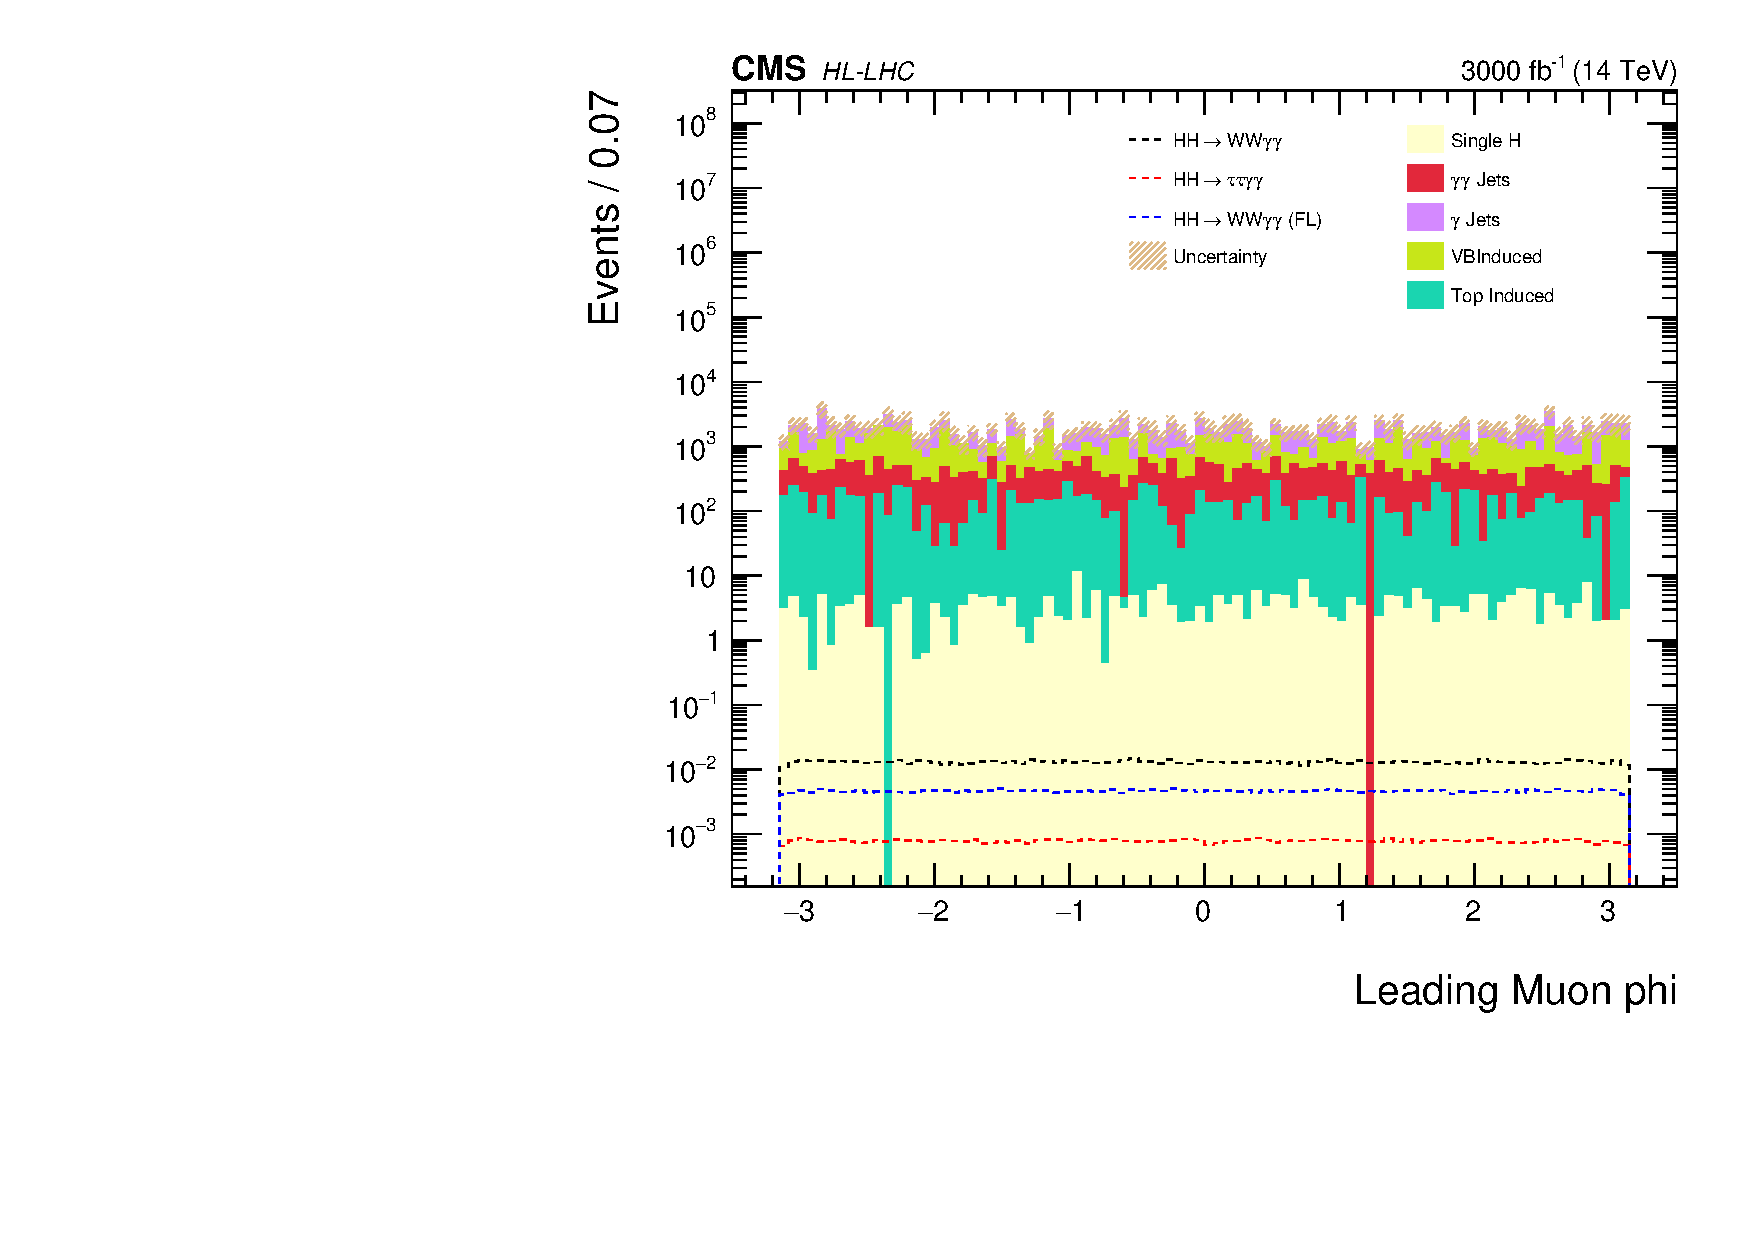
\includegraphics[width=\textwidth]{MuonPhi_logy.pdf}
        \vspace{-0.5cm}
        \firstsubcaption{Leading Muon $\phi$}
    \end{subfigure}
    \hfill
    \begin{subfigure}[b]{0.475\textwidth}   
        \centering 
        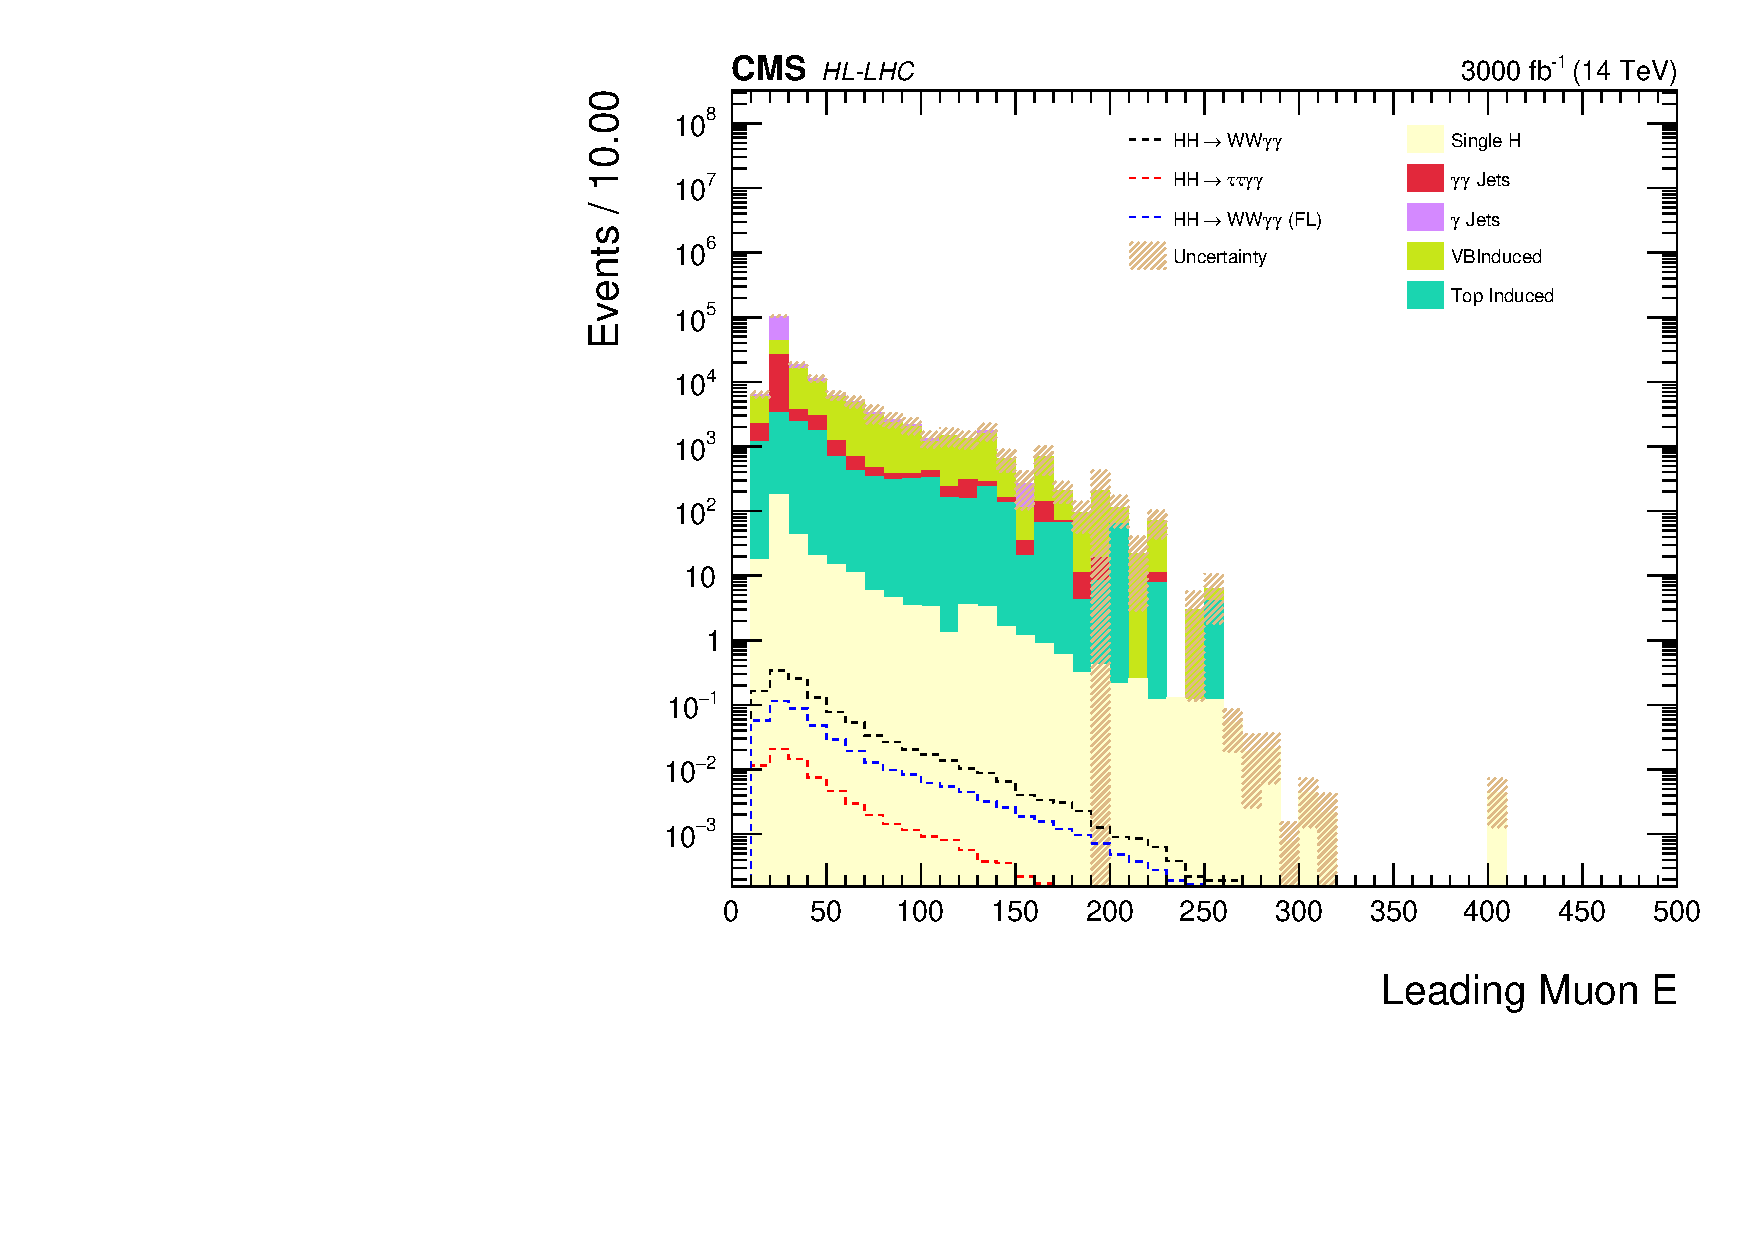
\includegraphics[width=\textwidth]{MuonE_logy.pdf}
        \vspace{-0.5cm}
        \firstsubcaption{Leading Muon energy}
    \end{subfigure}
    \vskip\baselineskip
    \begin{subfigure}[b]{0.475\textwidth}   
        \centering 
        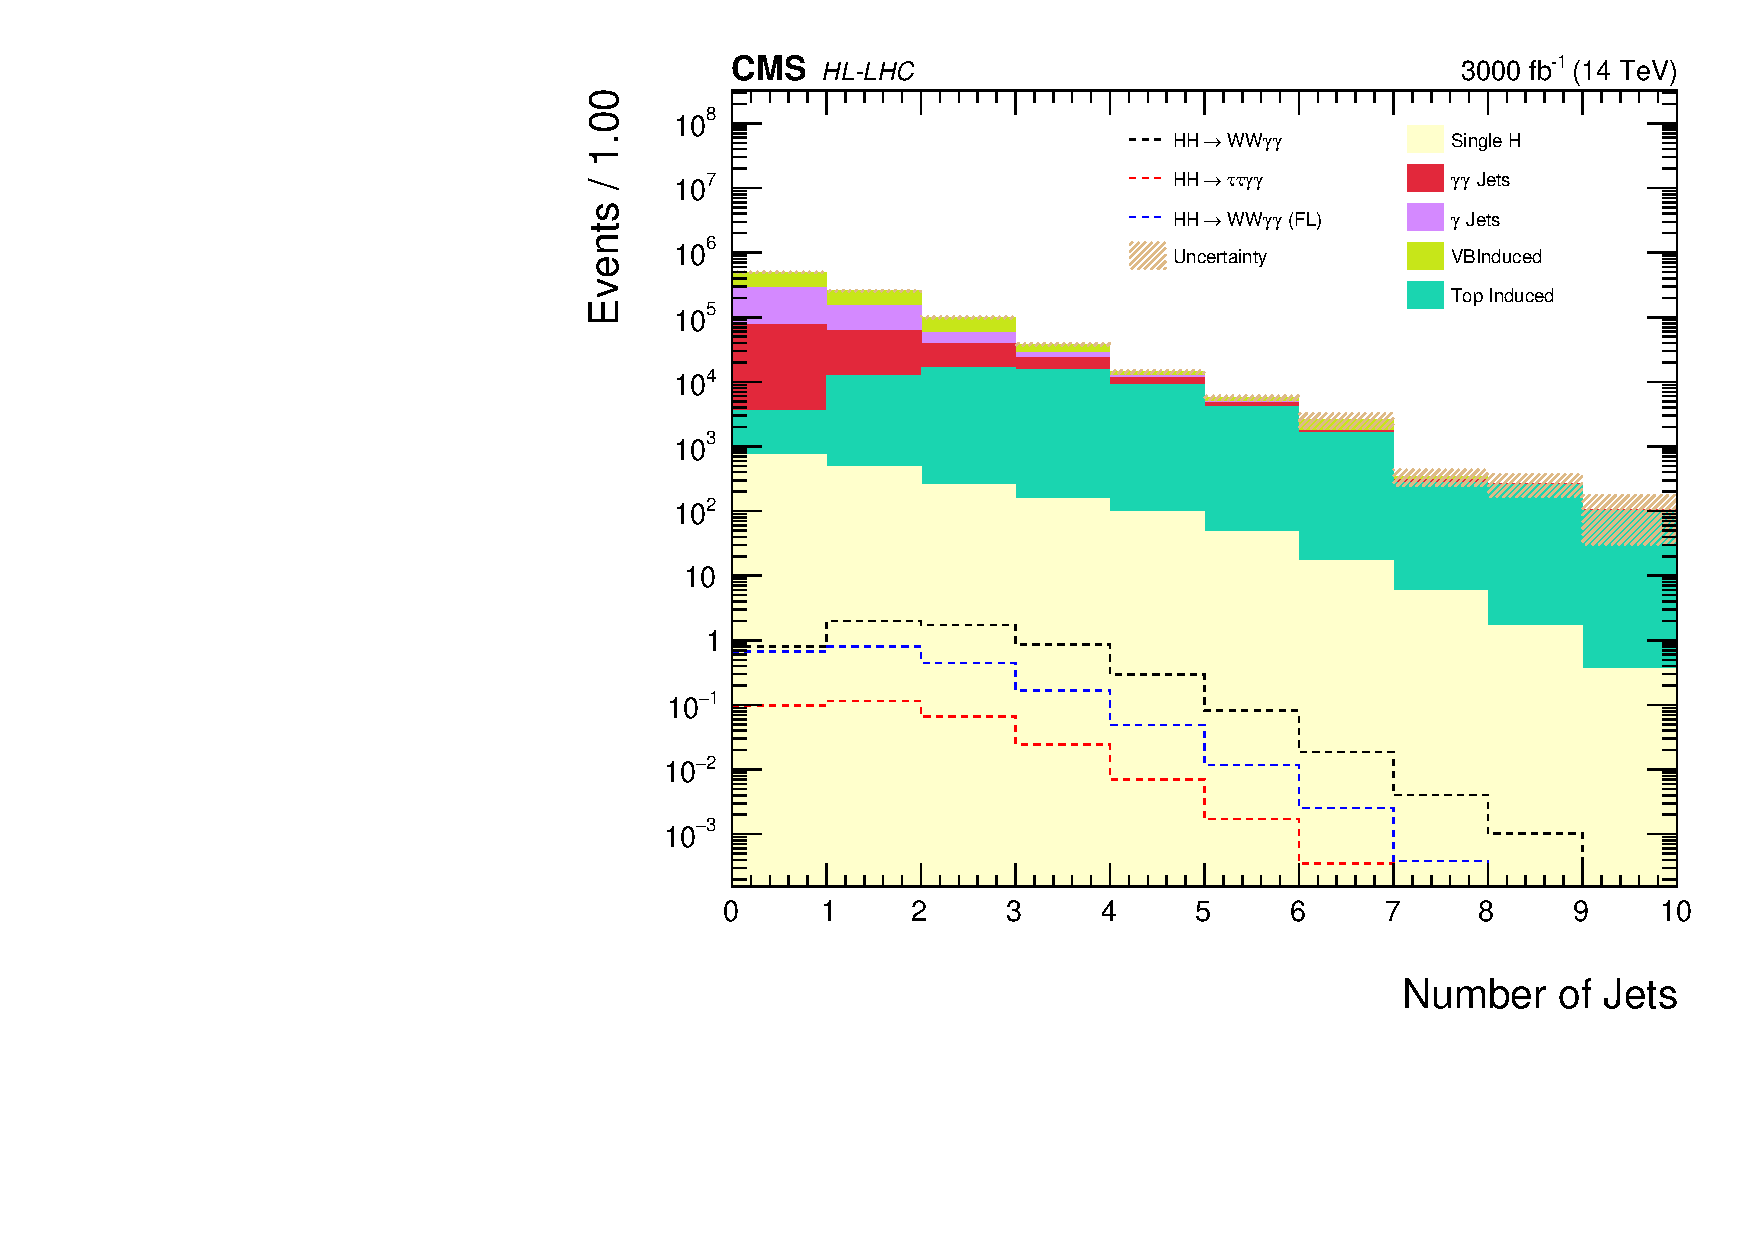
\includegraphics[width=\textwidth]{nJetsOneL_logy.pdf}
        \vspace{-0.5cm}
        \firstsubcaption{Jet multiplicity}
    \end{subfigure}
    \hfill
    \begin{subfigure}[b]{0.475\textwidth}   
        \centering 
        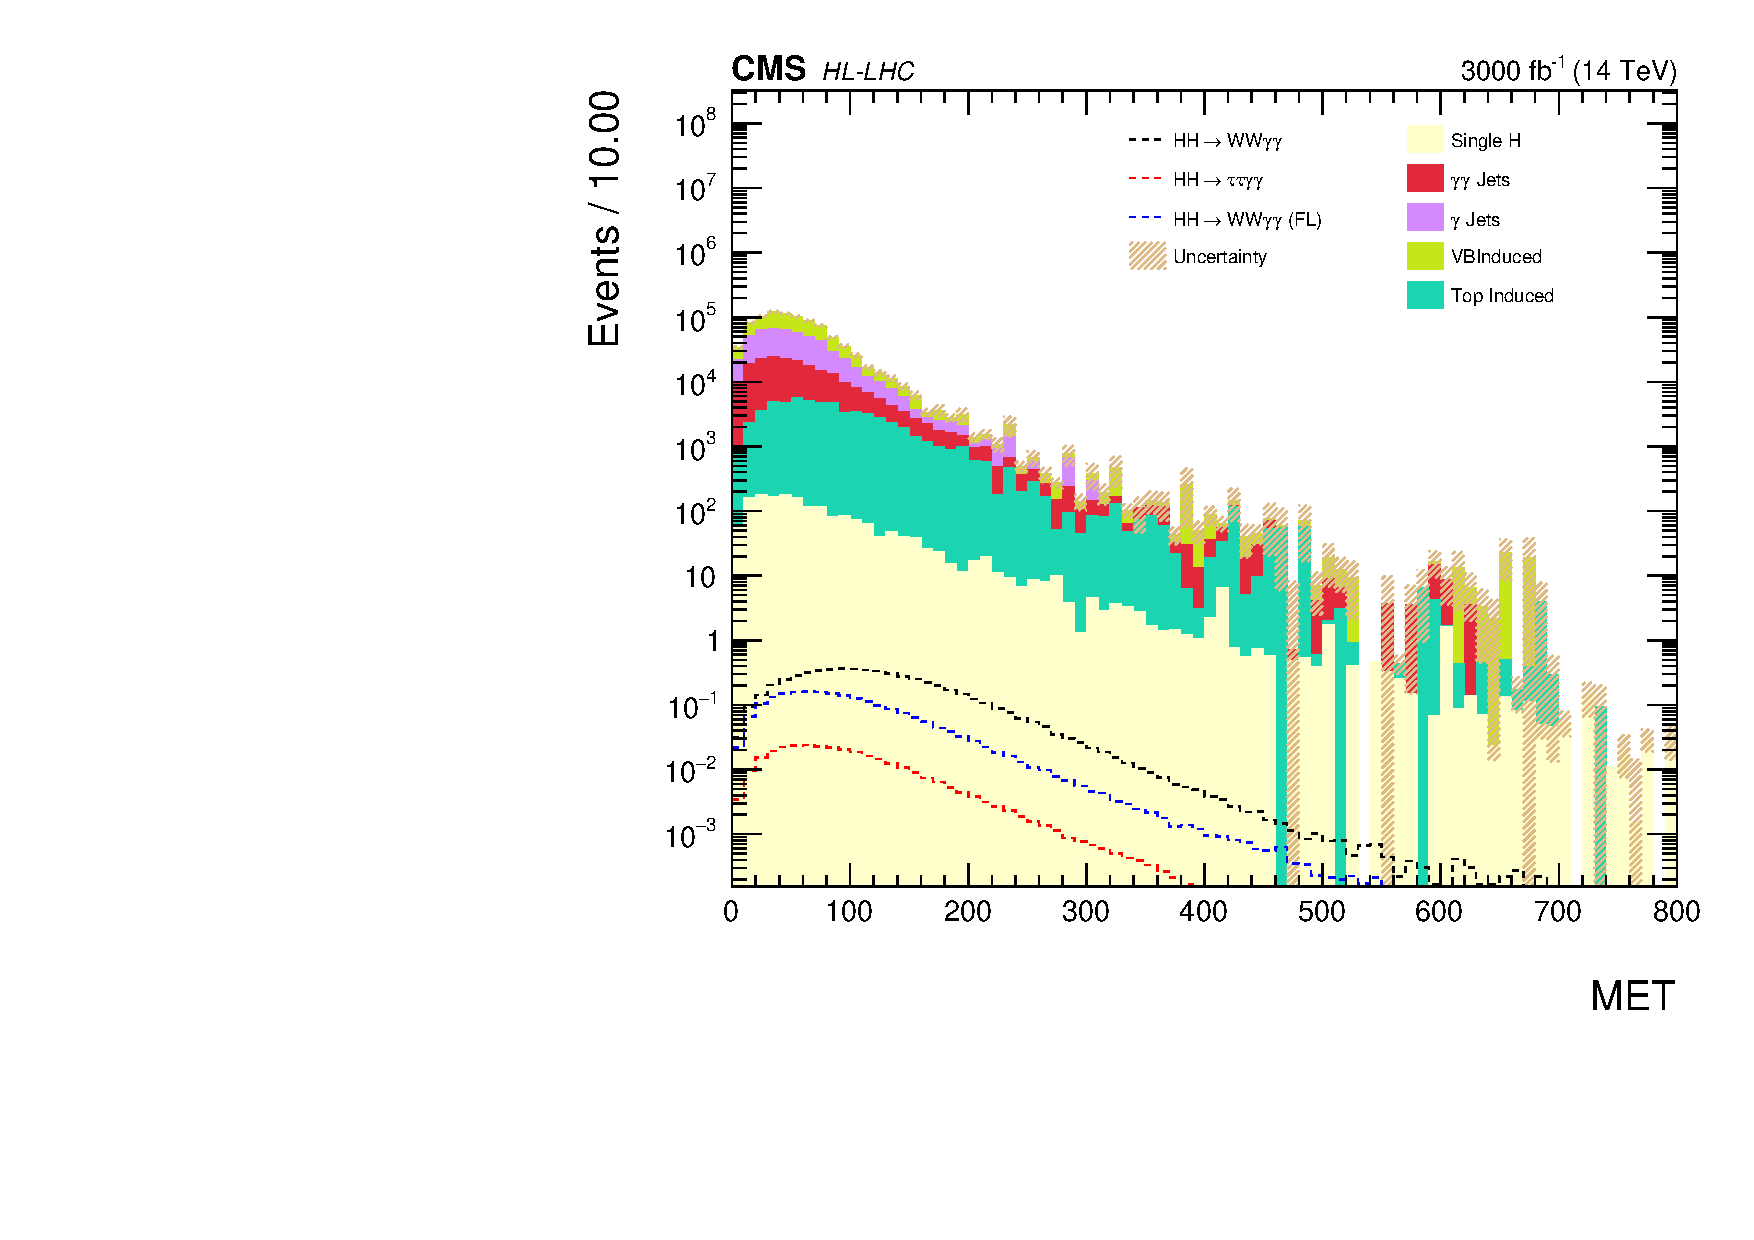
\includegraphics[width=\textwidth]{MET_logy.pdf}
        \vspace{-0.5cm}
        \firstsubcaption{$E_T^{miss}$}   
    \end{subfigure}
    \caption{\small DNN input distributions for the semi-leptonic channel of $HH\rightarrow{WW\gamma\gamma}$ (continued).}
\end{figure*}

\begin{figure*}[h!]
    \centering
    \begin{subfigure}[b]{0.475\textwidth}
        \centering
        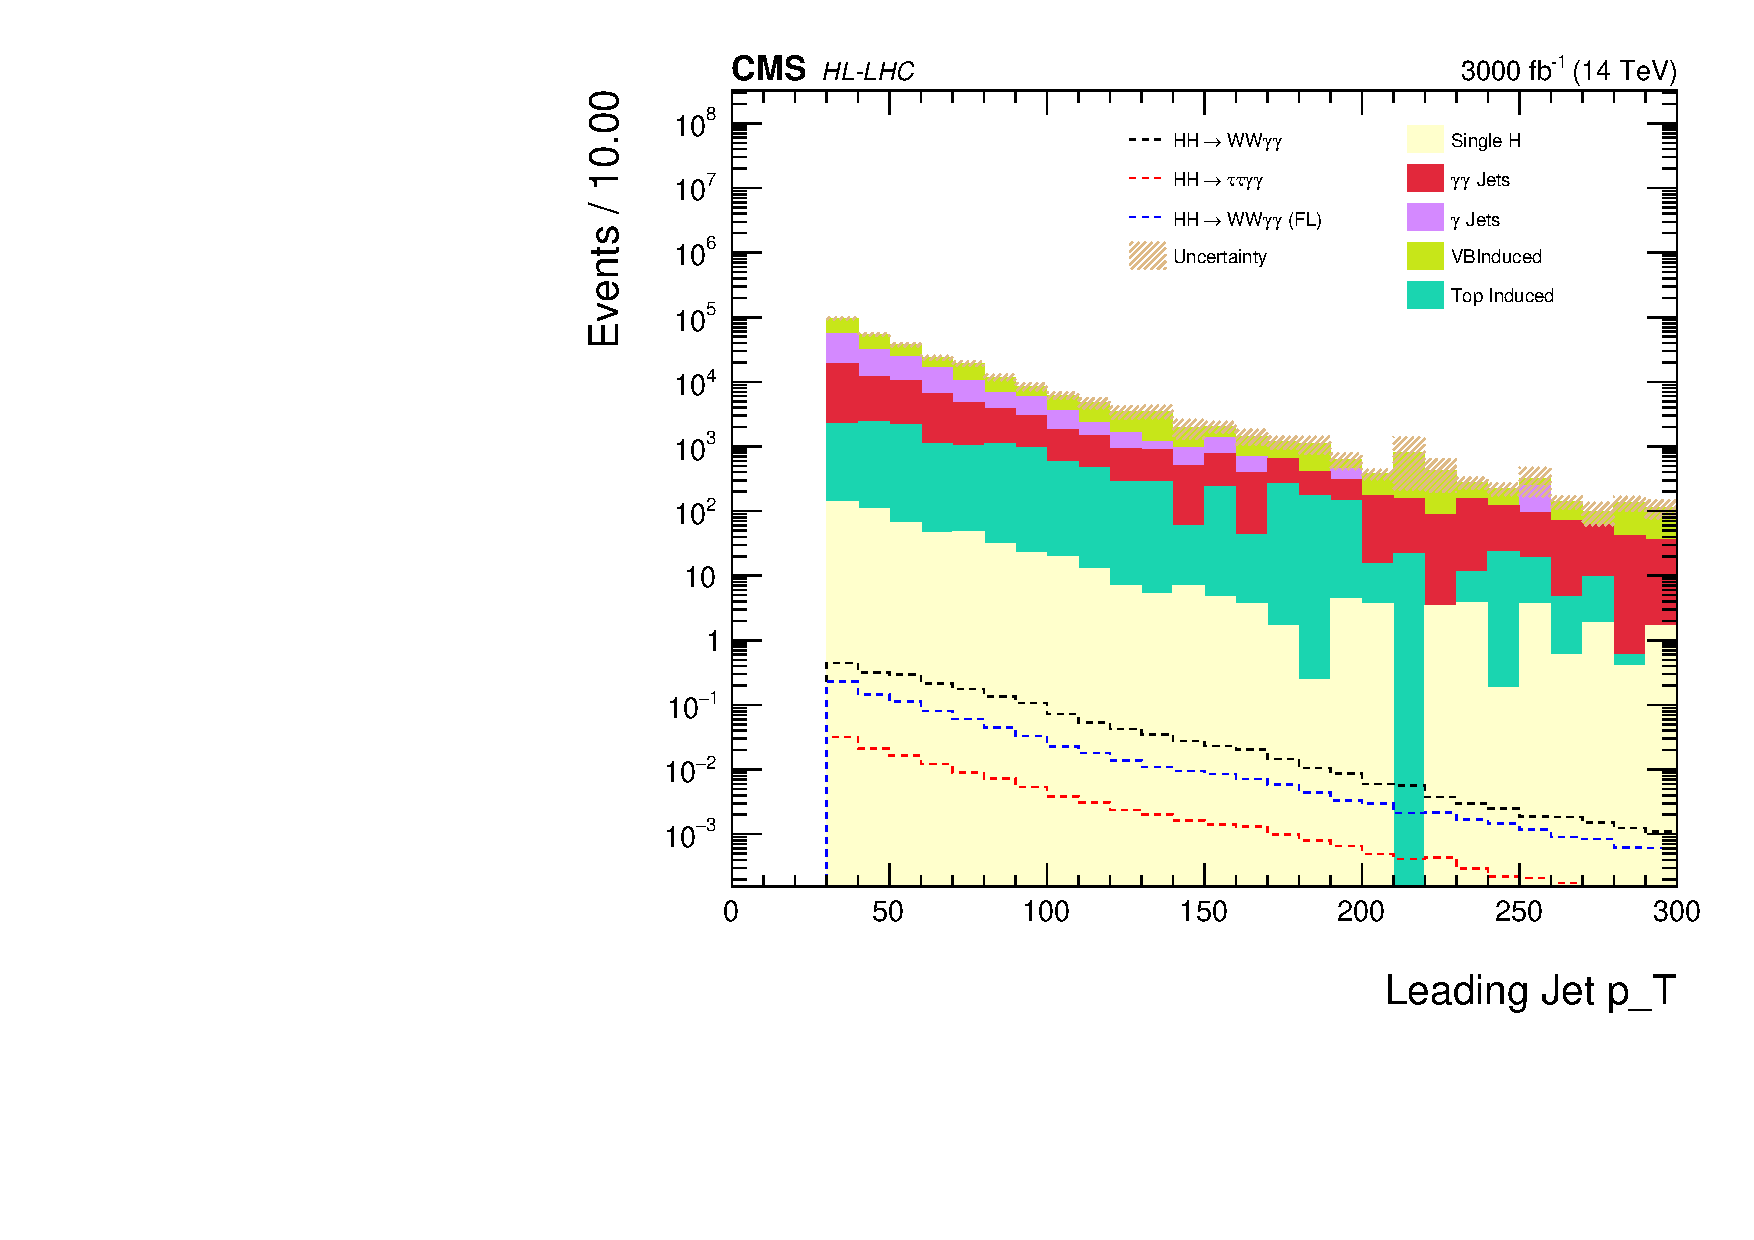
\includegraphics[width=\textwidth]{hasonel_hasOneJ_jetpt_logy.pdf}
        \vspace{-0.5cm}
        \firstsubcaption{Leading jet \pt}
    \end{subfigure}
    \hfill
    \begin{subfigure}[b]{0.475\textwidth}  
        \centering 
        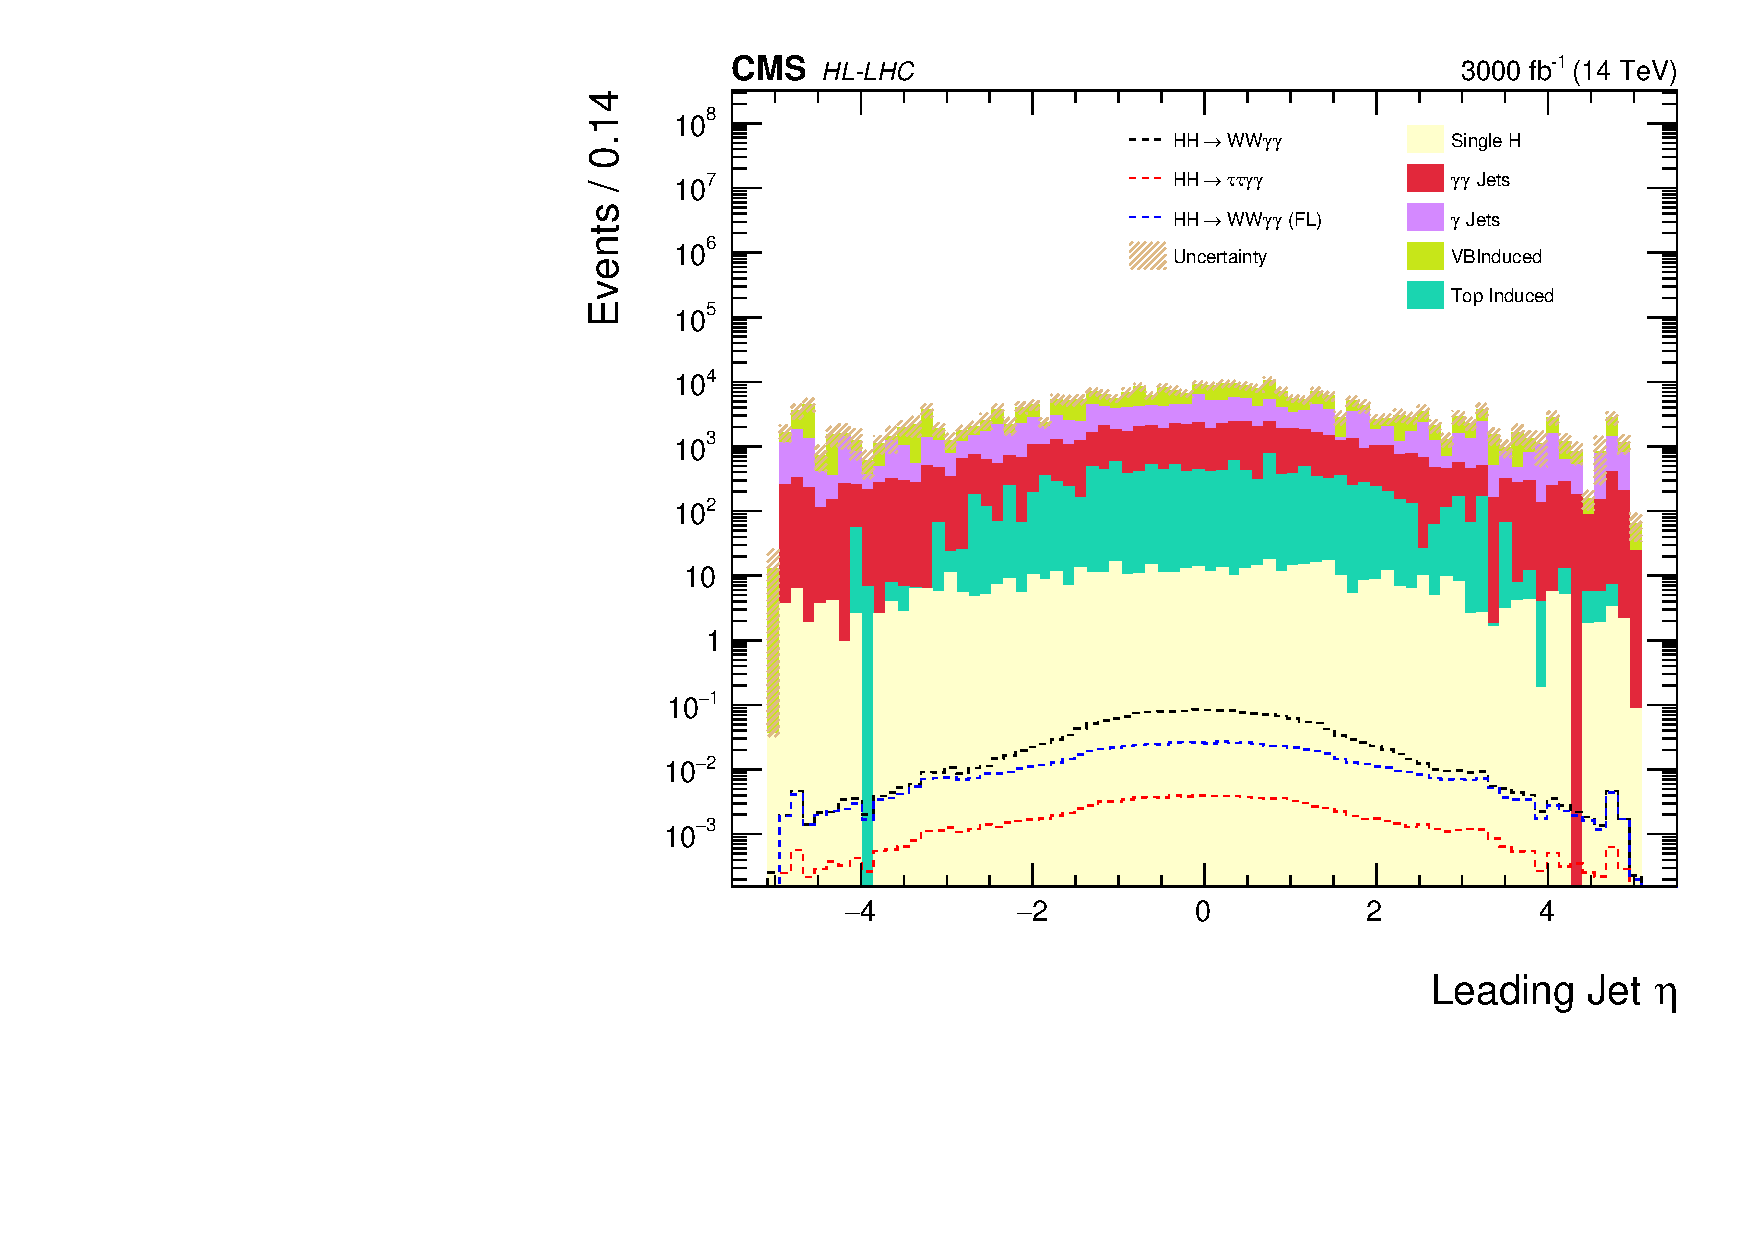
\includegraphics[width=\textwidth]{hasonel_hasOneJ_jeteta_logy.pdf}
        \vspace{-0.5cm}
        \firstsubcaption{Leading jet $\eta$}
    \end{subfigure}
    \vskip\baselineskip
    \begin{subfigure}[b]{0.475\textwidth}   
        \centering 
        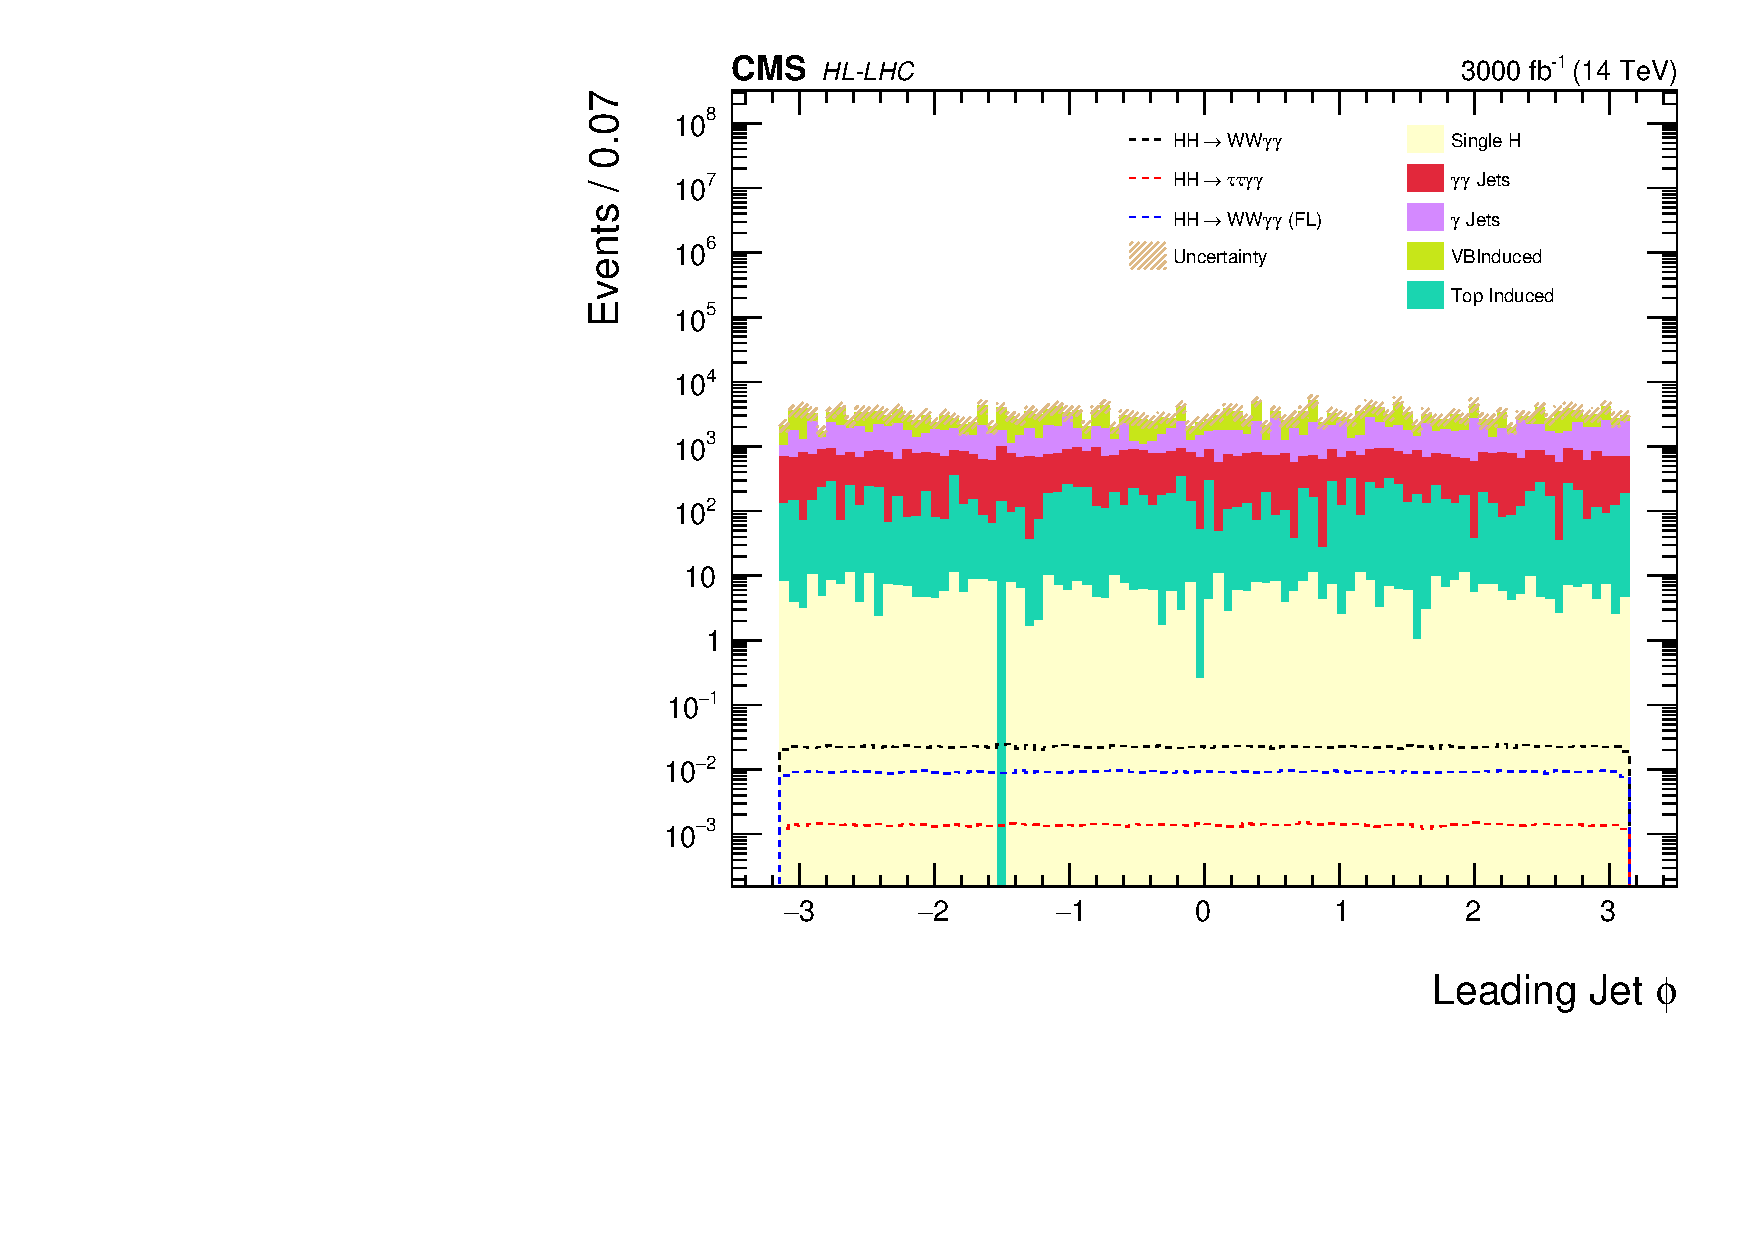
\includegraphics[width=\textwidth]{hasonel_hasOneJ_jetphi_logy.pdf}
        \vspace{-0.5cm}
        \firstsubcaption{Leading jet $\phi$}
    \end{subfigure}
    \hfill
    \begin{subfigure}[b]{0.475\textwidth}   
        \centering 
        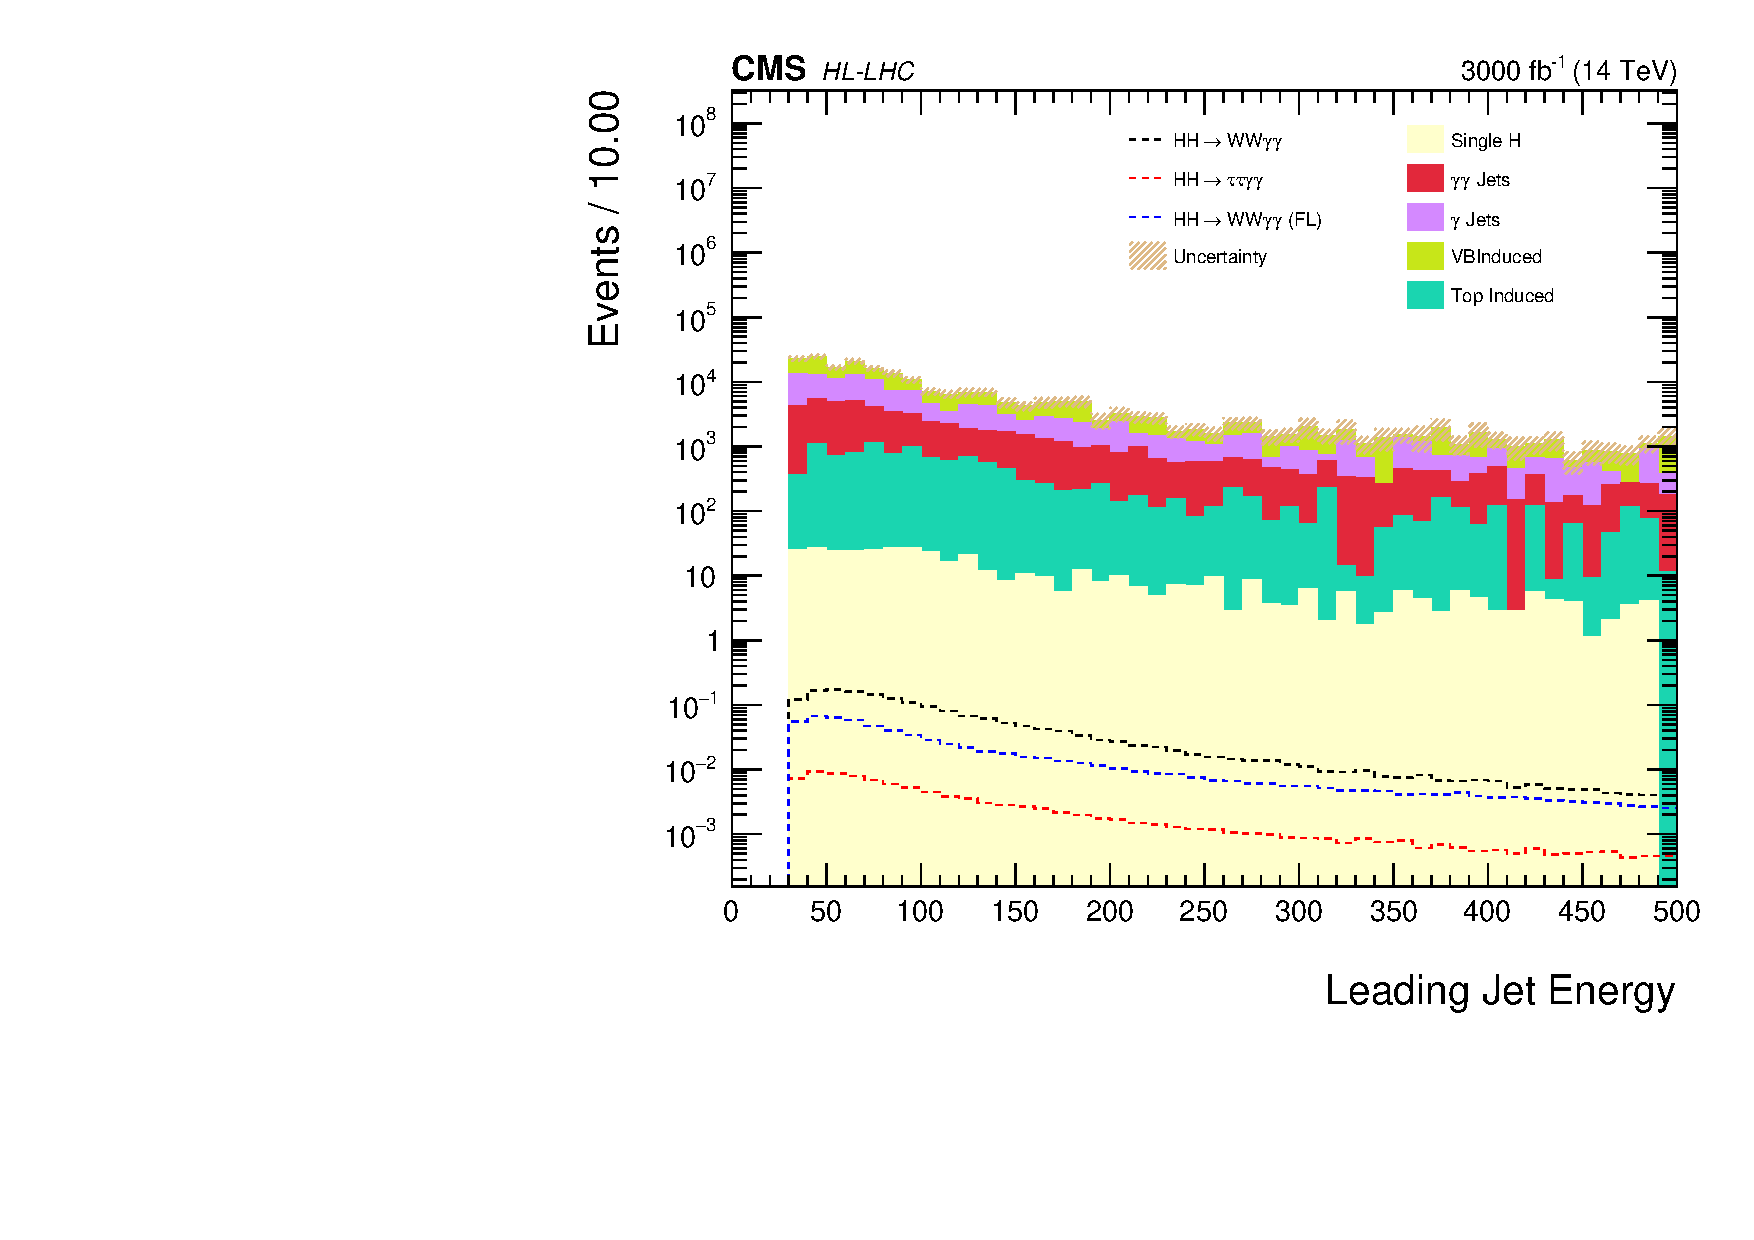
\includegraphics[width=\textwidth]{hasonel_hasOneJ_jetE_logy.pdf}
        \vspace{-0.5cm}
        \firstsubcaption{Leading jet energy}
    \end{subfigure}
    \vskip\baselineskip
    \begin{subfigure}[b]{0.475\textwidth}   
        \centering 
        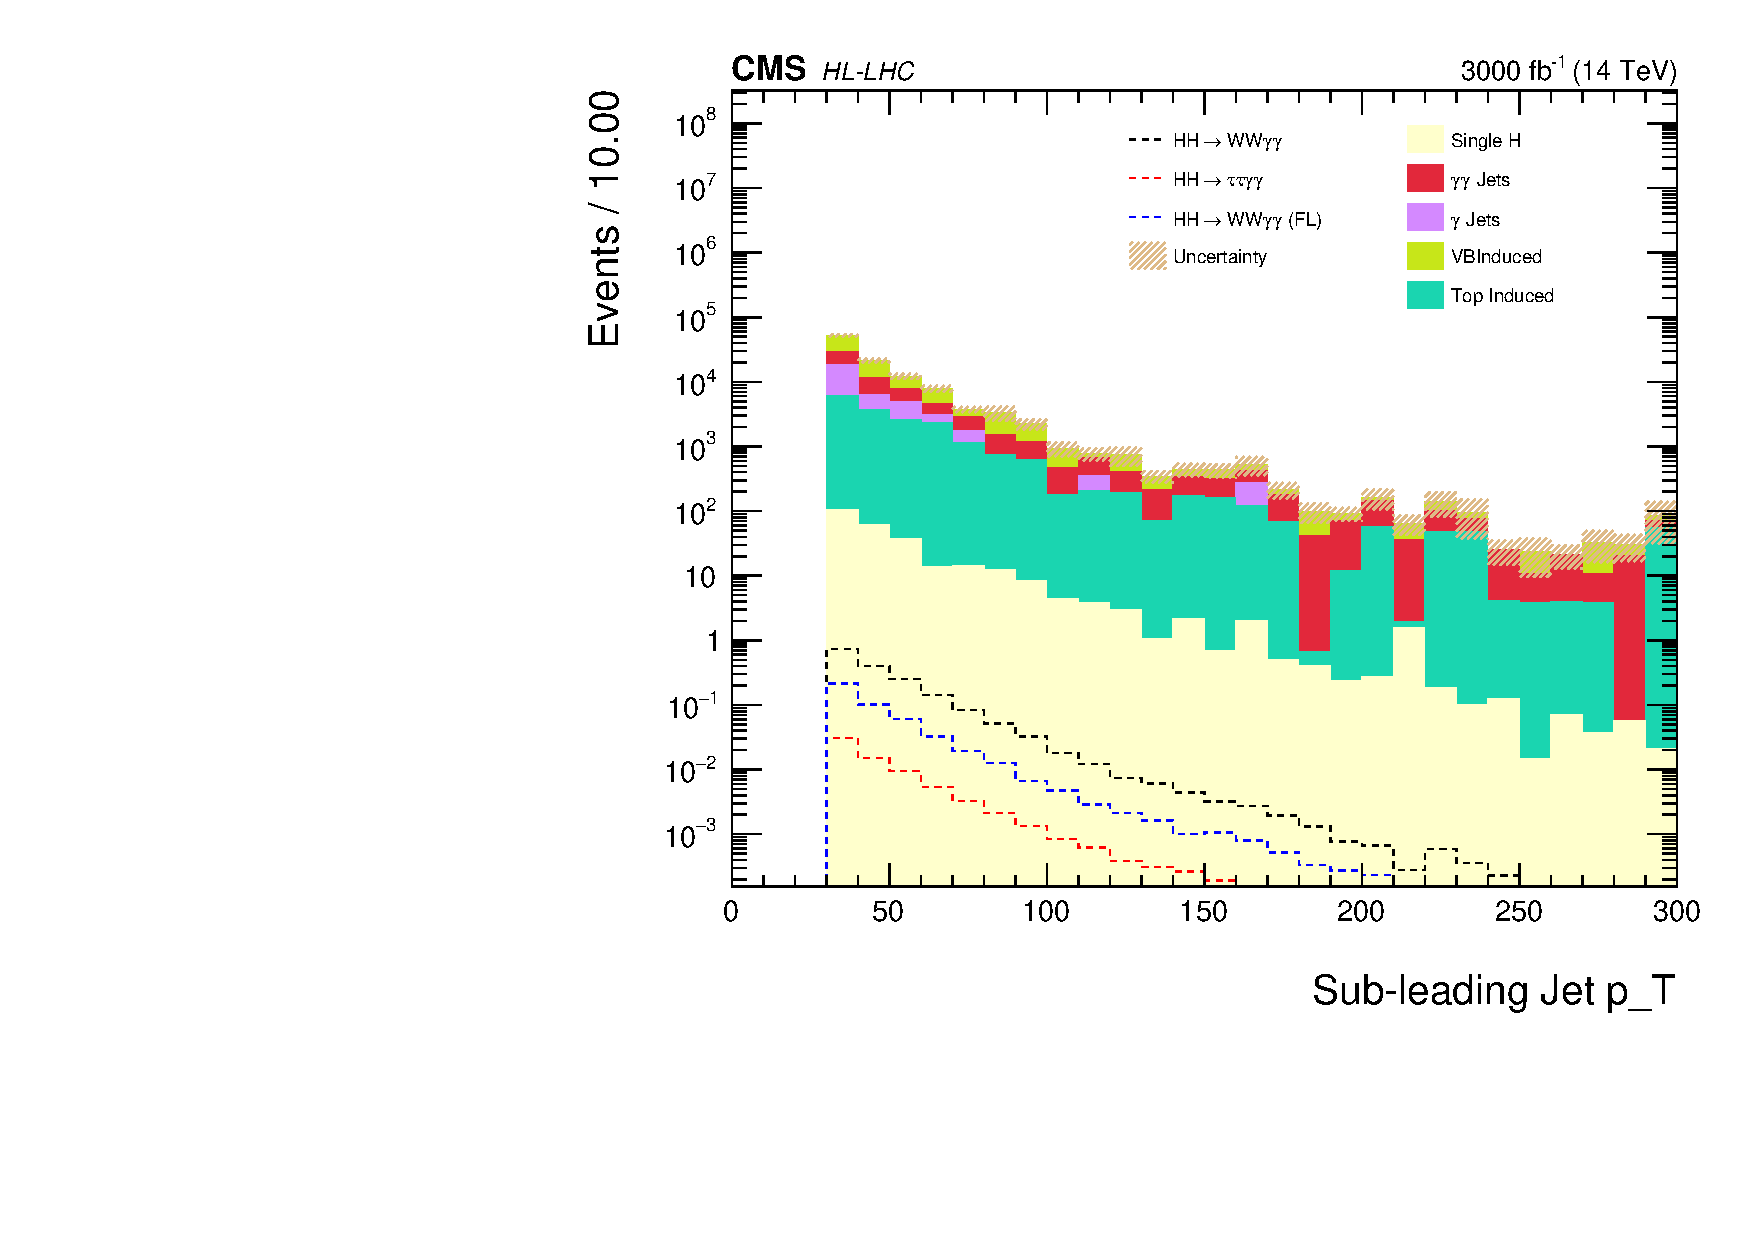
\includegraphics[width=\textwidth]{hasonel_hasTwoJ_jetpt_logy.pdf}
        \vspace{-0.5cm}
        \firstsubcaption{Sub-leading jet \pt}
    \end{subfigure}
    \hfill
    \begin{subfigure}[b]{0.475\textwidth}   
        \centering 
        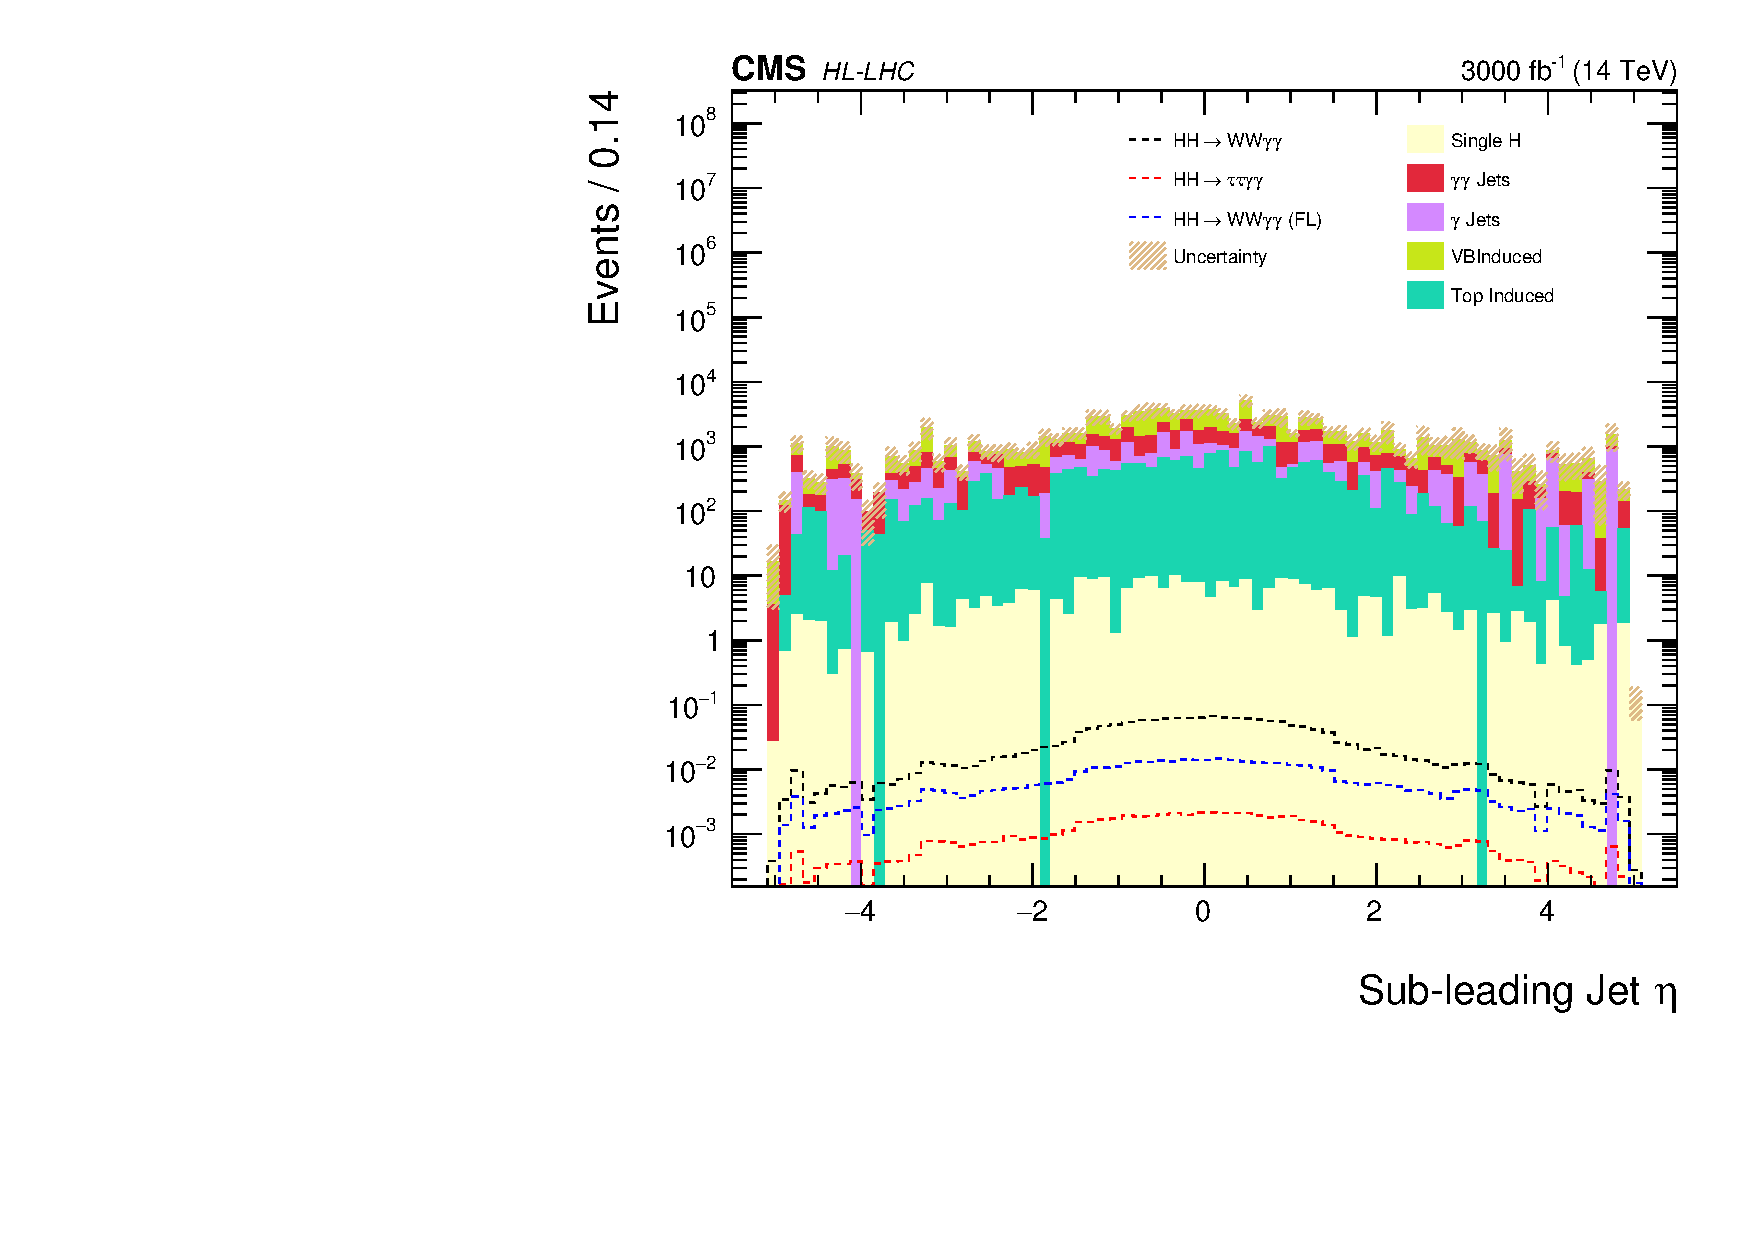
\includegraphics[width=\textwidth]{hasonel_hasTwoJ_jeteta_logy.pdf}
        \vspace{-0.5cm}
        \firstsubcaption{Sub-leading jet $\eta$}   
    \end{subfigure}
    \caption{\small DNN input distributions for the semi-leptonic channel of $HH\rightarrow{WW\gamma\gamma}$ (continued).}
\end{figure*}

\begin{figure*}[h!]
    \centering
    \begin{subfigure}[b]{0.475\textwidth}
        \centering
        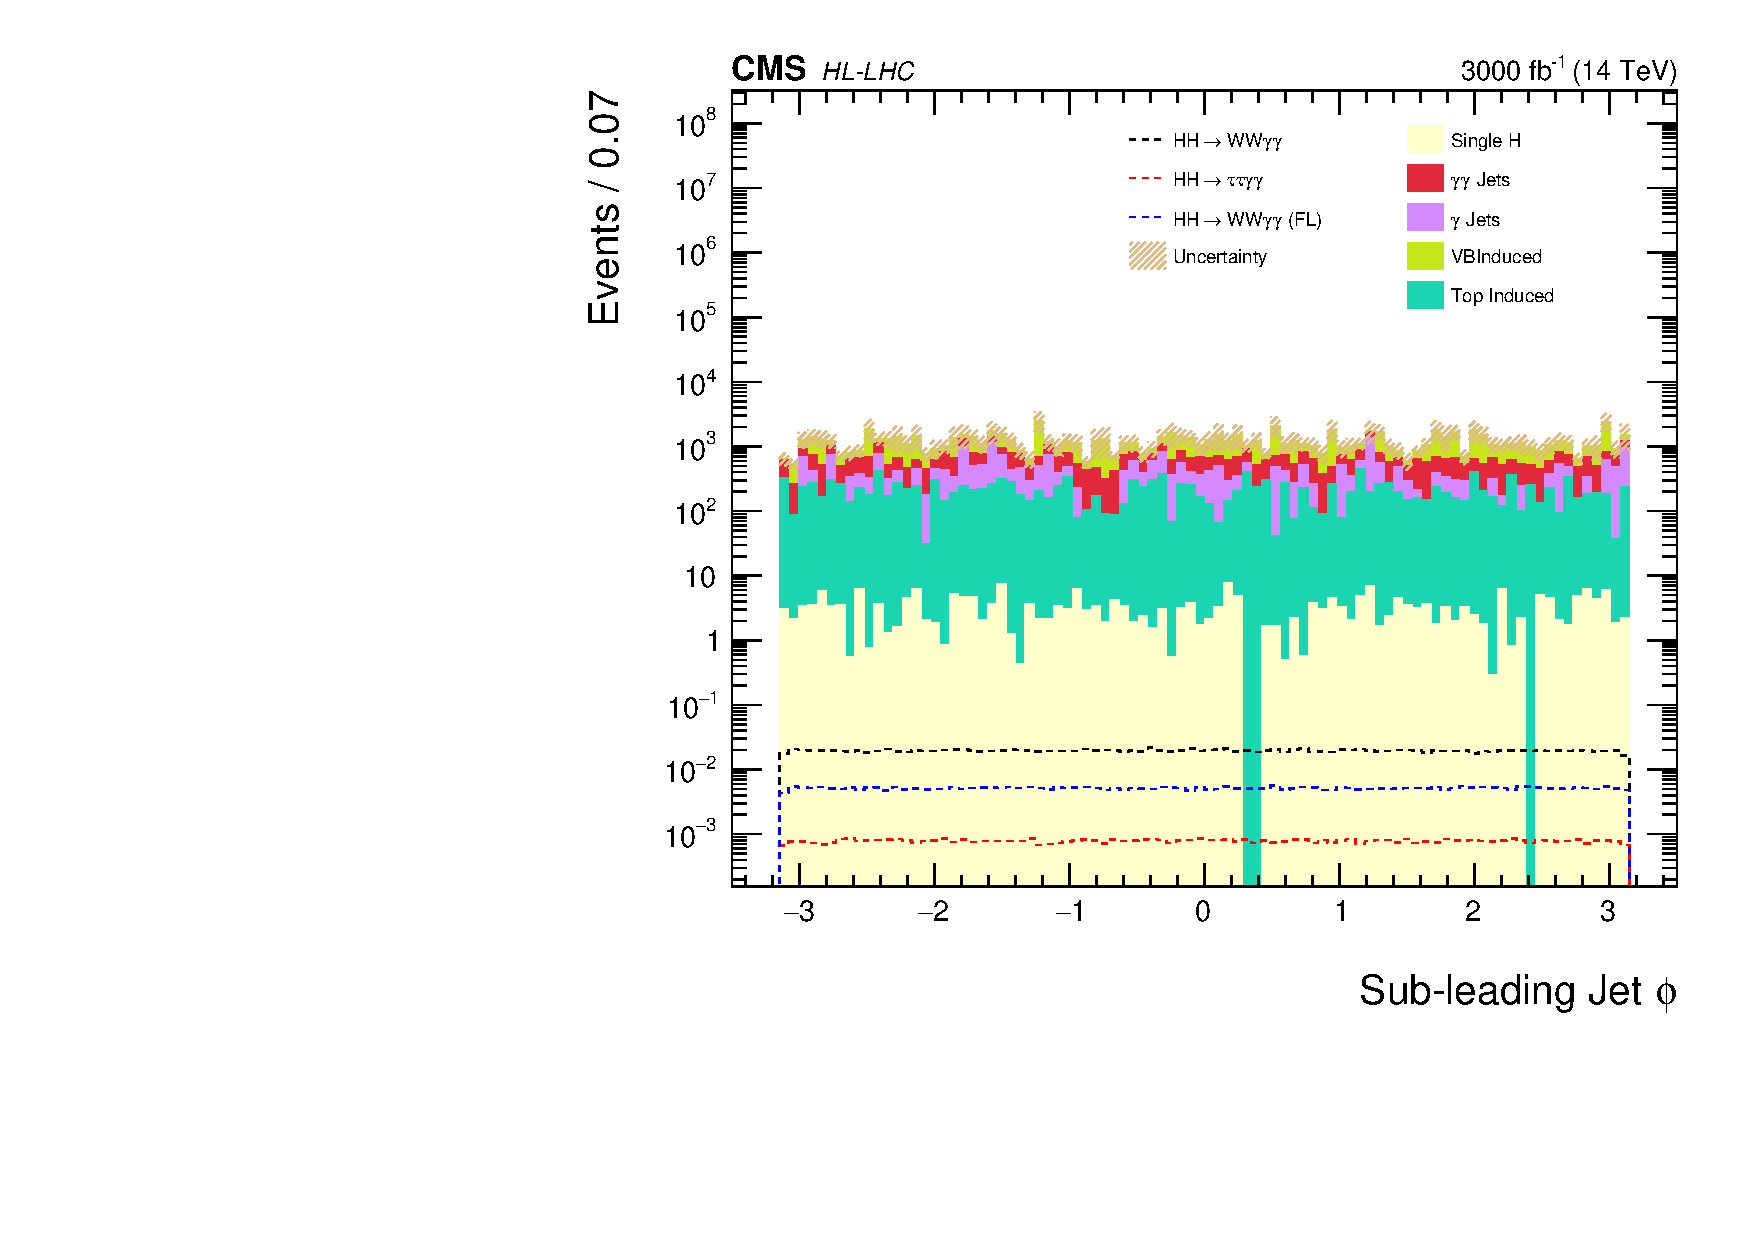
\includegraphics[width=\textwidth]{hasonel_hasTwoJ_jetphi_logy.pdf}
        \vspace{-0.5cm}
        \firstsubcaption{Sub-leading jet $\phi$}
    \end{subfigure}
    \hfill
    \begin{subfigure}[b]{0.475\textwidth}  
        \centering 
        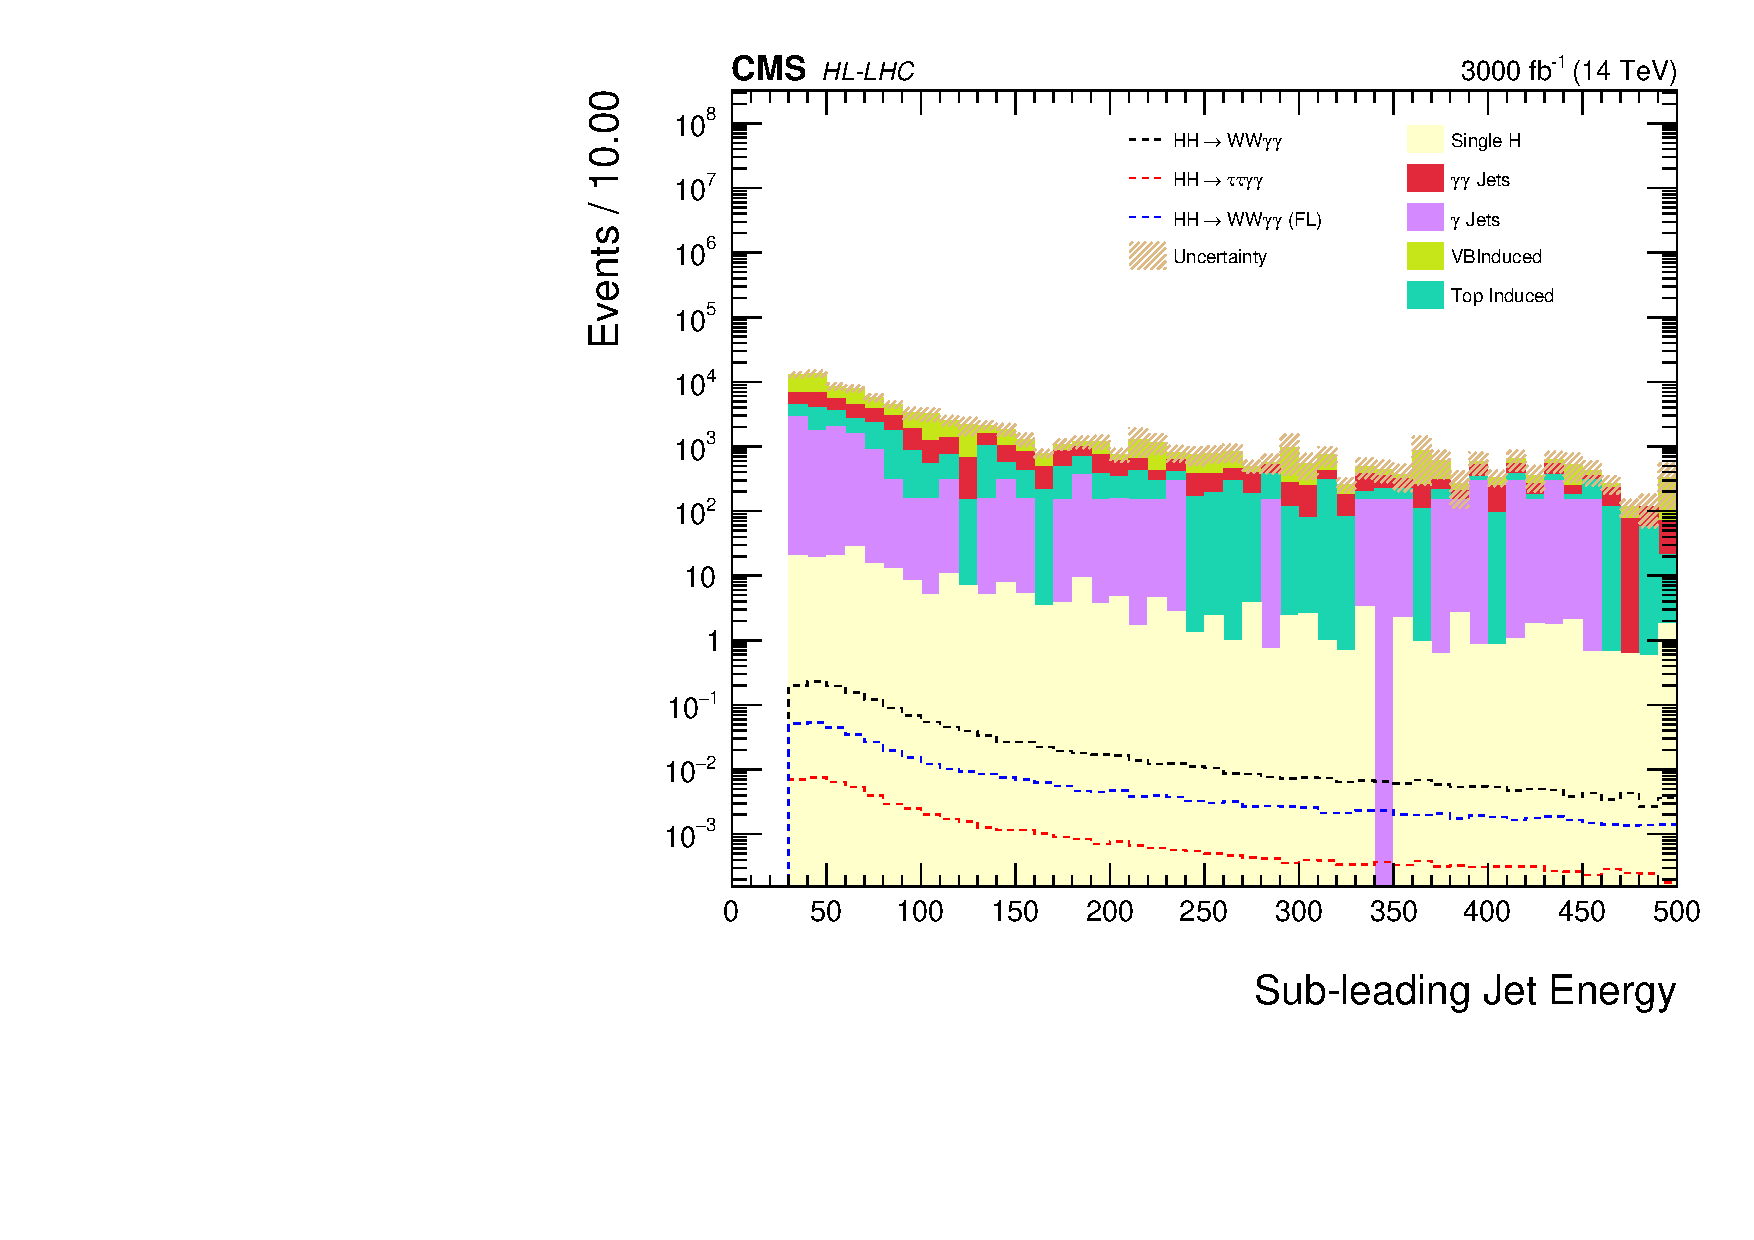
\includegraphics[width=\textwidth]{hasonel_hasTwoJ_jetE_logy.pdf}
        \vspace{-0.5cm}
        \firstsubcaption{Sub-leading jet energy}
    \end{subfigure}
    \vskip\baselineskip
    \begin{subfigure}[b]{0.475\textwidth}   
        \centering 
        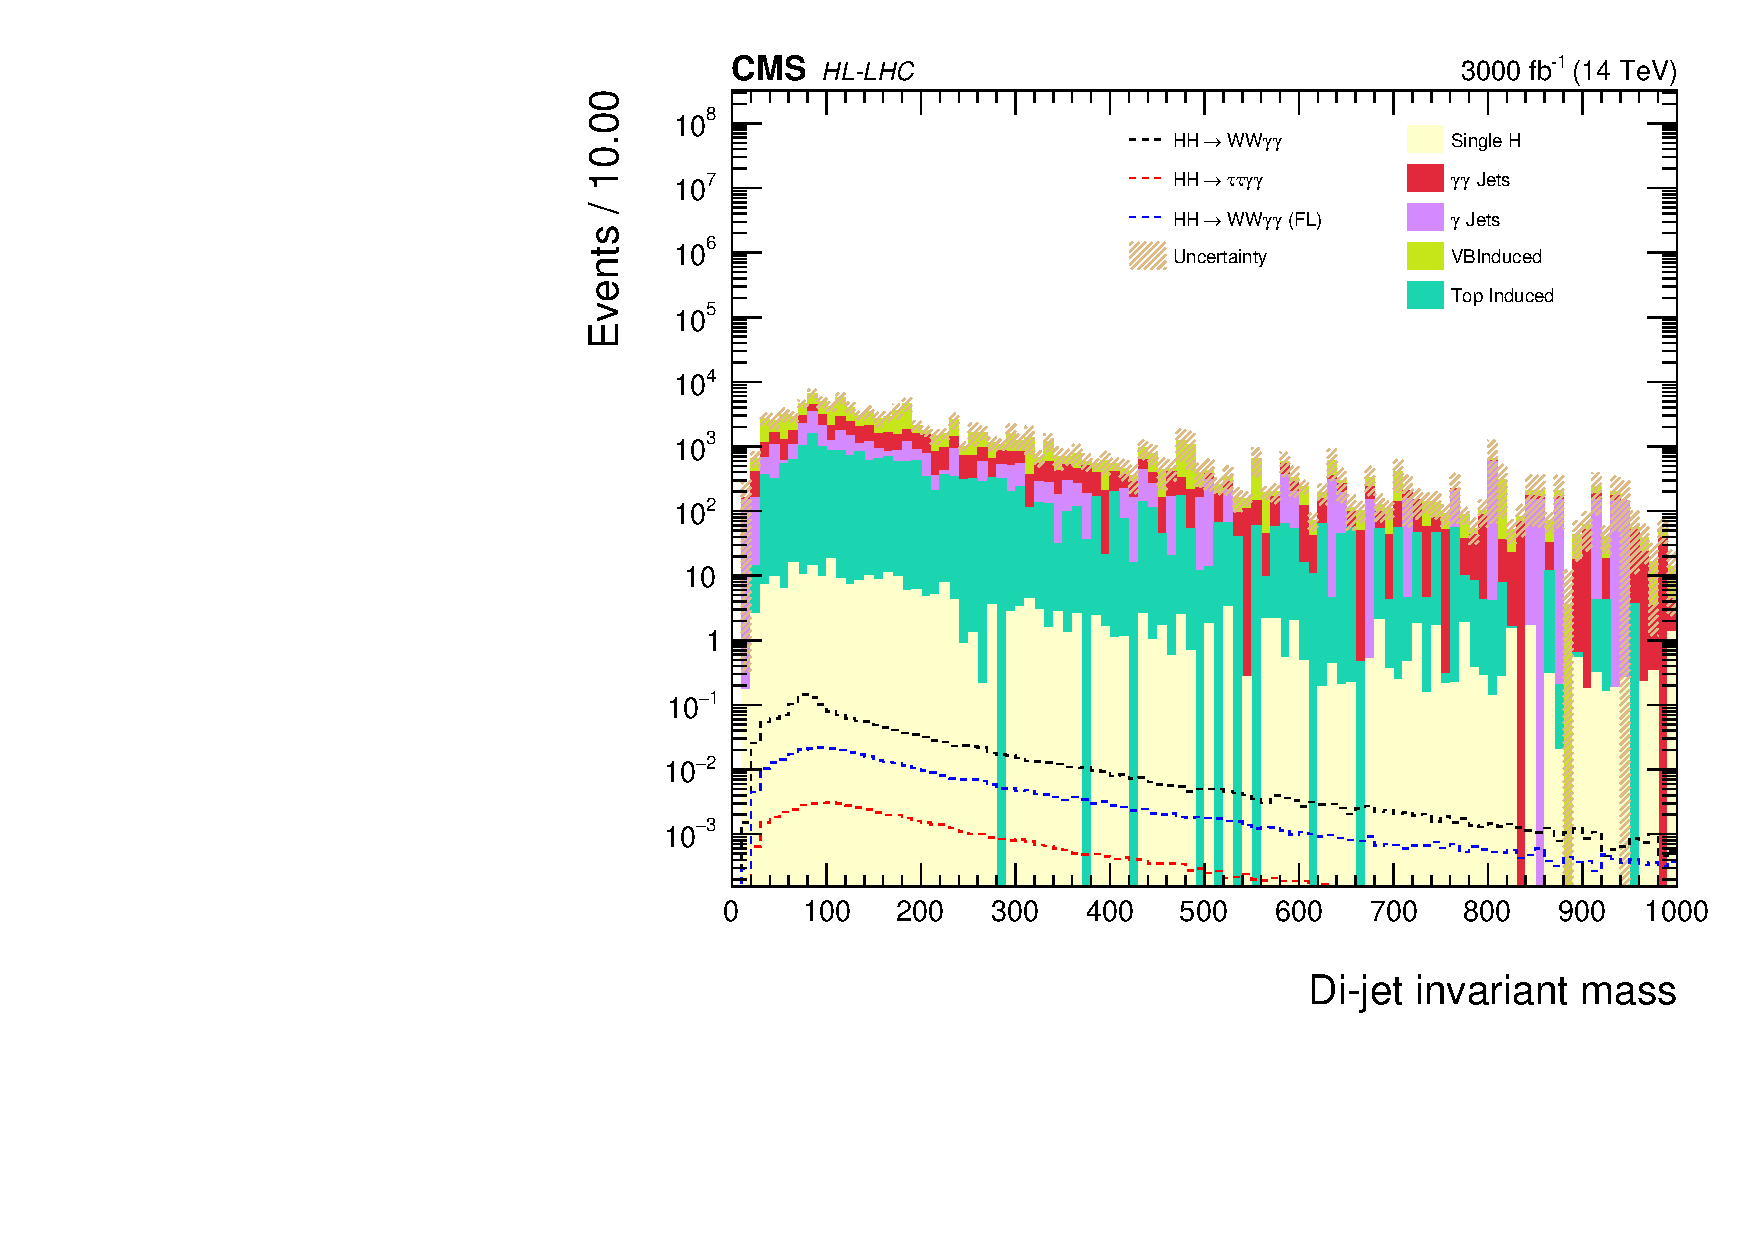
\includegraphics[width=\textwidth]{hasonel_hastwoJ_mjj_logy.pdf}
        \vspace{-0.5cm}
        \firstsubcaption{$m_{j_0,j_1}$}
    \end{subfigure}
    \hfill
    \begin{subfigure}[b]{0.475\textwidth}   
        \centering 
        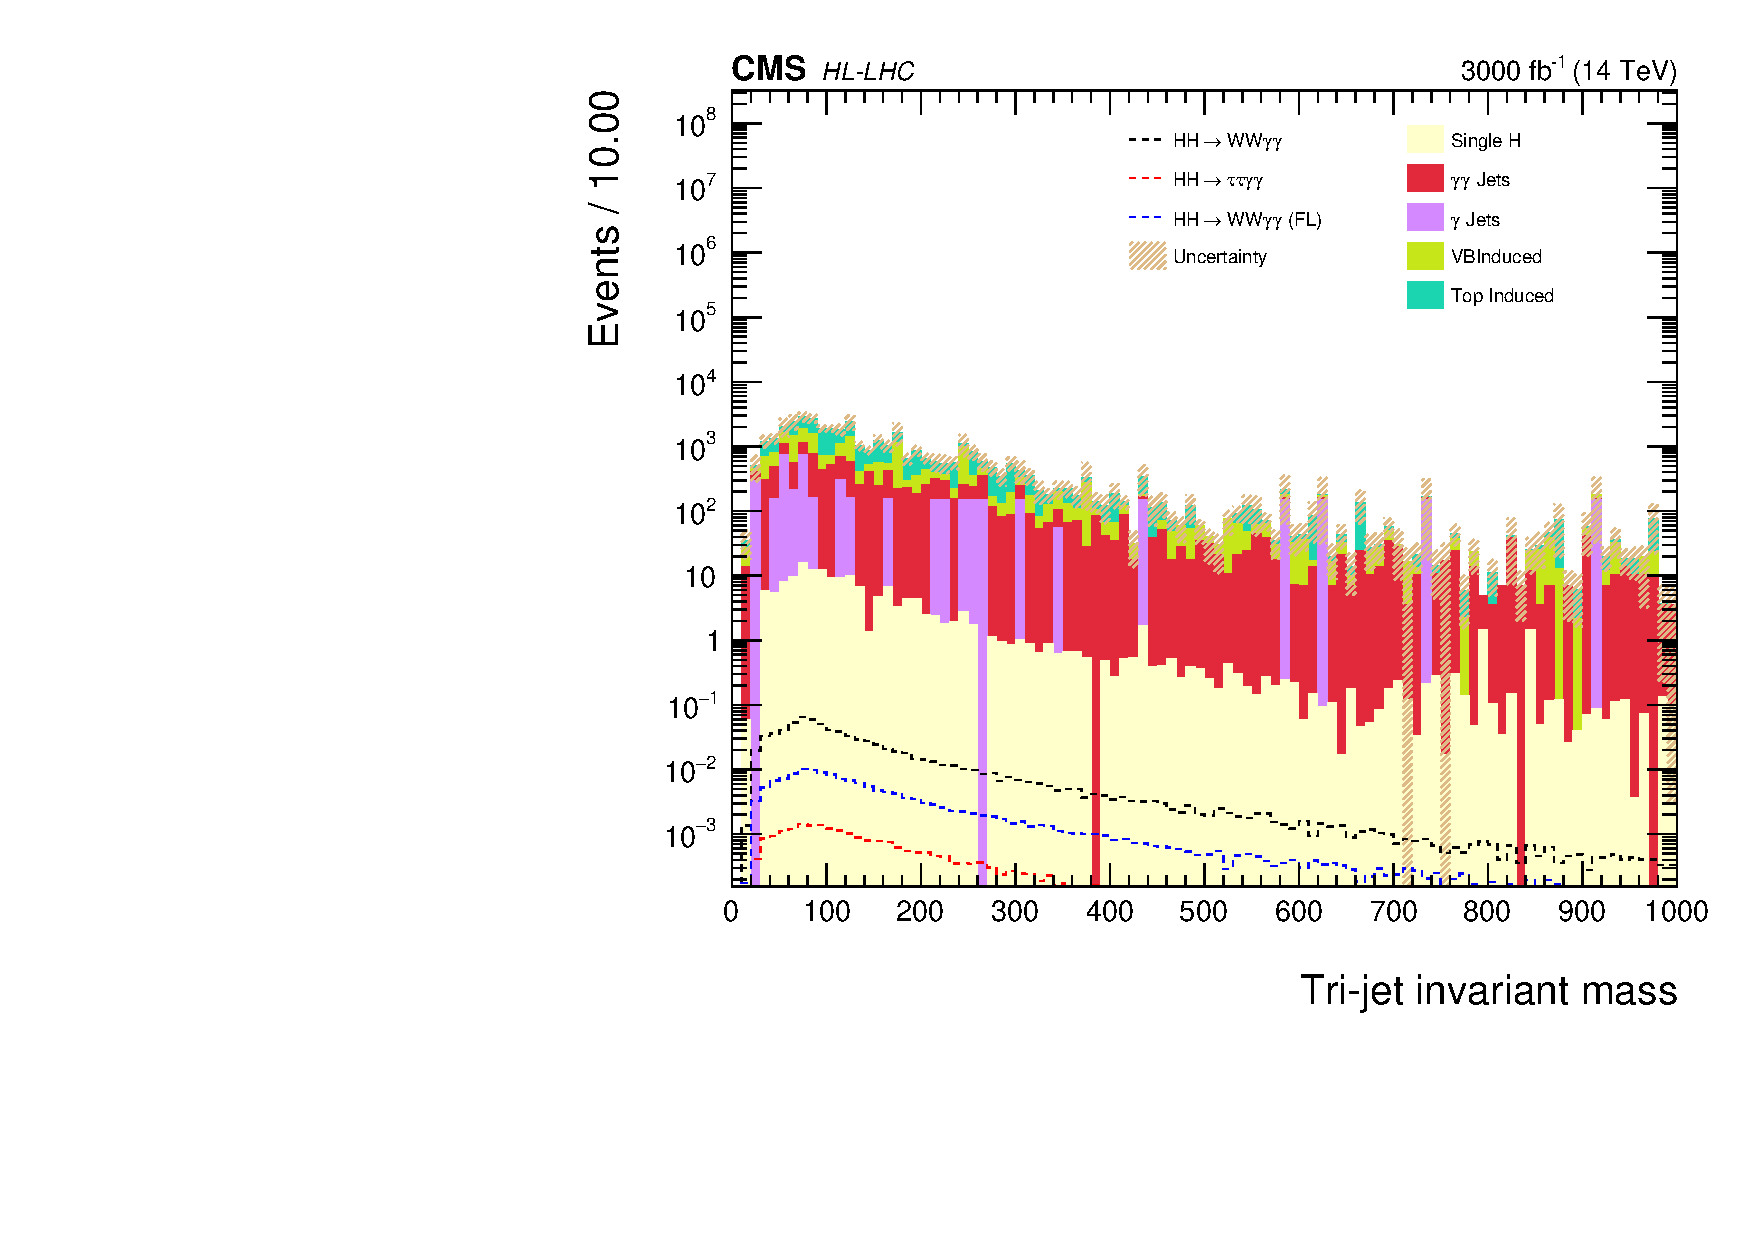
\includegraphics[width=\textwidth]{hasonel_hasthreeJ_mjj_logy.pdf}
        \vspace{-0.5cm}
        \firstsubcaption{$m_{j_1,j_2}$}
    \end{subfigure}
    \vskip\baselineskip
    \begin{subfigure}[b]{0.475\textwidth}   
        \centering 
        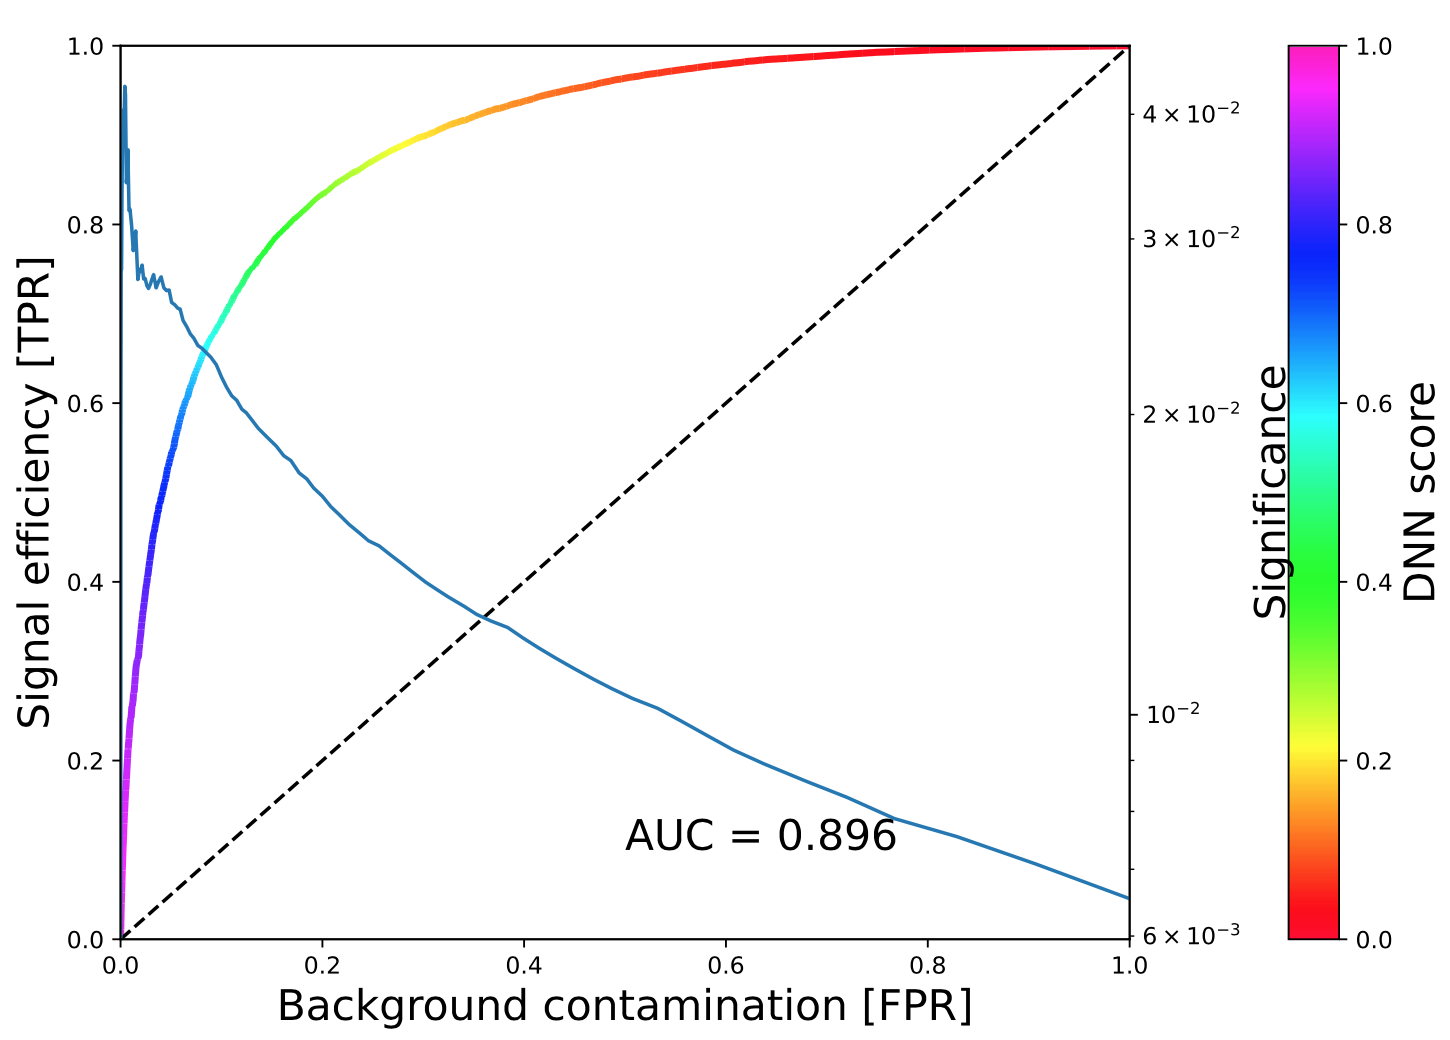
\includegraphics[width=\textwidth]{SLodd_training_roc.png}
        \vspace{-0.5cm}
        \firstsubcaption{Odd training}
    \end{subfigure}
    \hfill
    \begin{subfigure}[b]{0.475\textwidth}   
        \centering 
        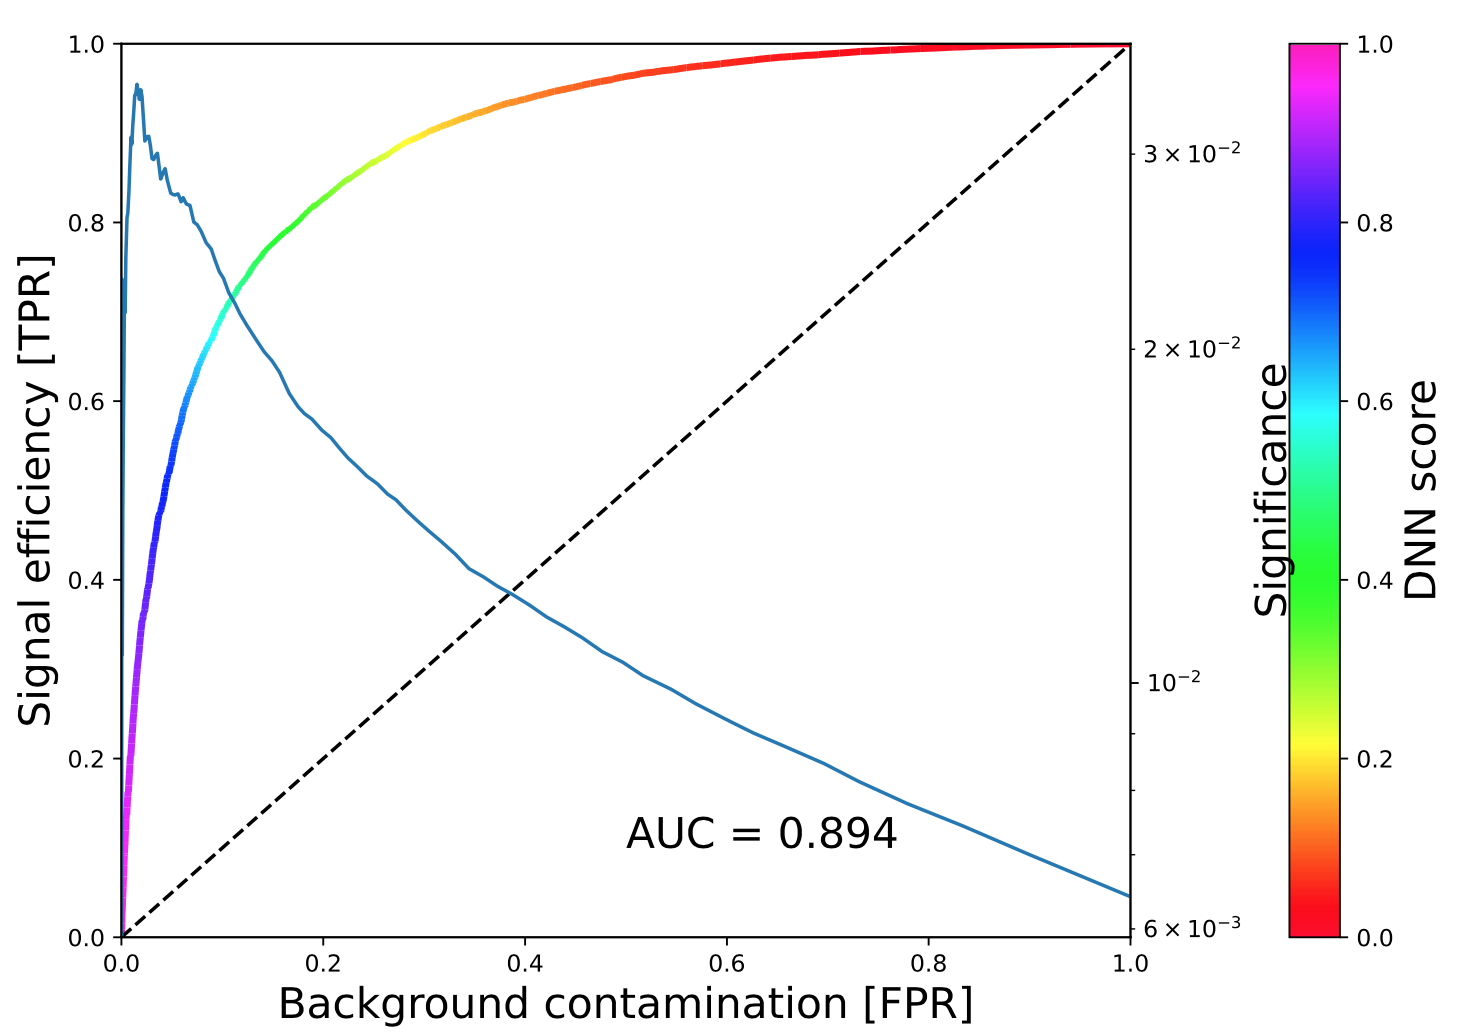
\includegraphics[width=\textwidth]{SLeven_training_roc.png}
        \vspace{-0.5cm} 
        \firstsubcaption{Even training}   
    \end{subfigure}
    \caption{\small DNN input distributions (a,b,c,d) and the ROC curves (e,f) for the semi-leptonic channel of $HH\rightarrow{WW\gamma\gamma}$ (continued).} 
\end{figure*}

\begin{figure*}[h!]
    \centering
    \begin{subfigure}[b]{0.475\textwidth}
        \centering
        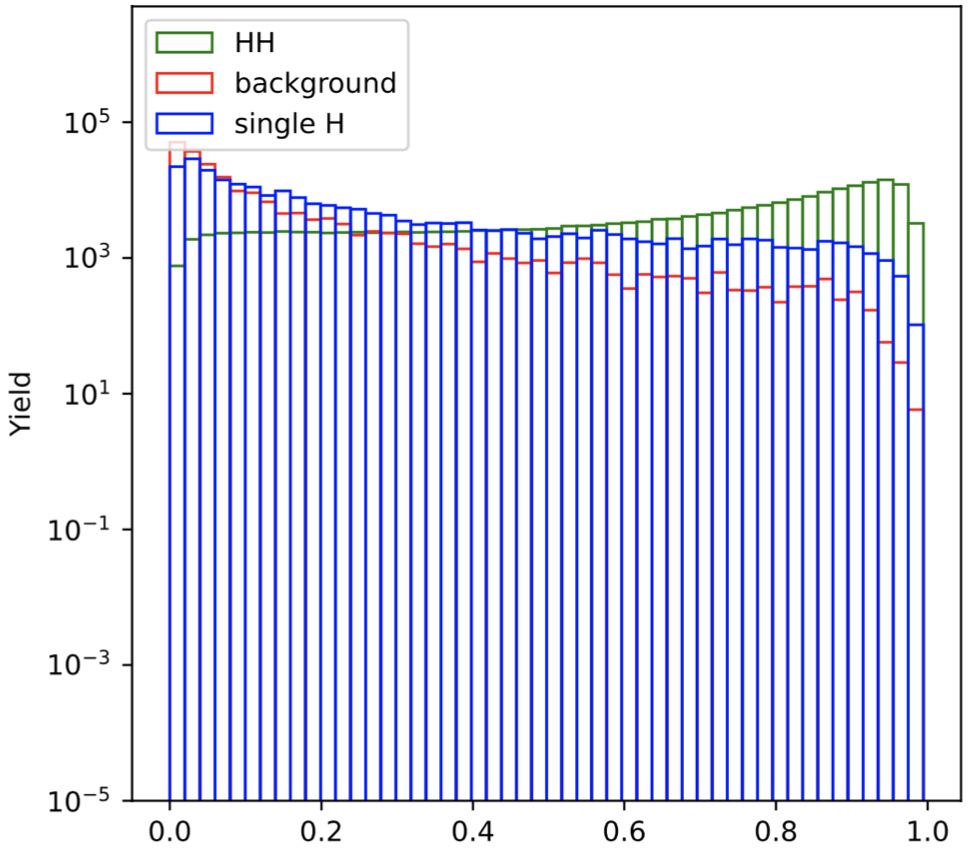
\includegraphics[width=\textwidth]{SLodd-weights.png}
        \vspace{-0.5cm}
        \firstsubcaption{Odd training}
    \end{subfigure}
    \hfill
    \begin{subfigure}[b]{0.475\textwidth}  
        \centering 
        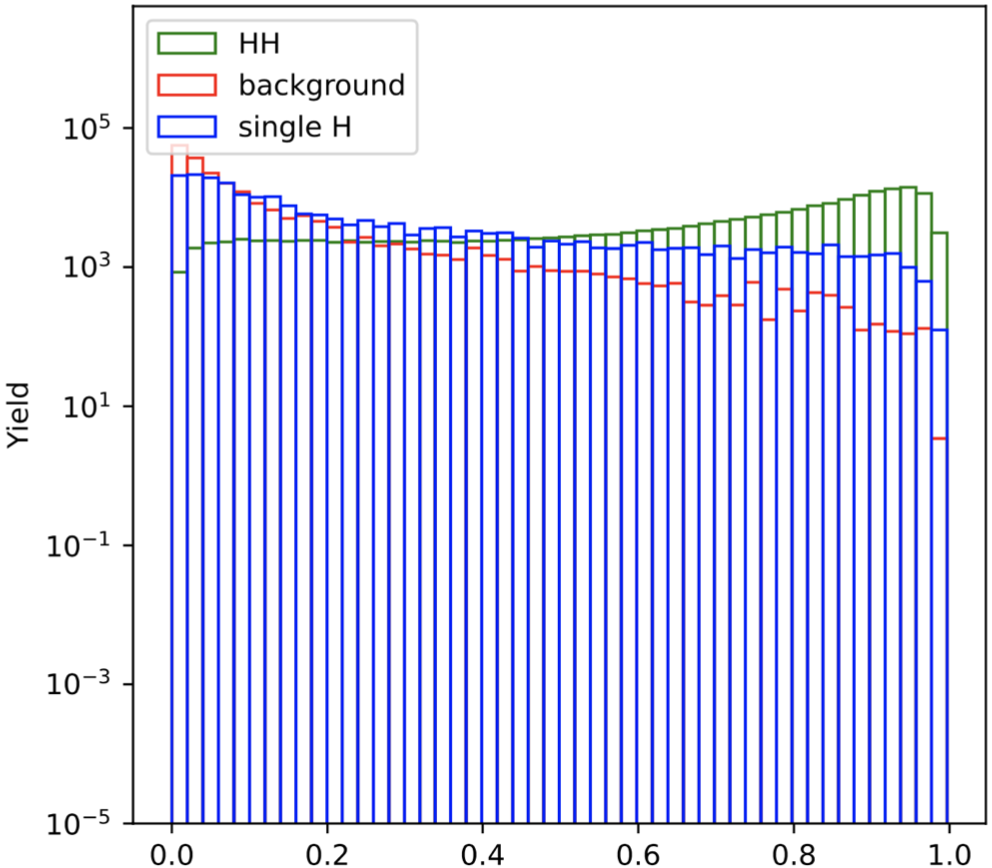
\includegraphics[width=\textwidth]{SLeven-weights.png}
        \vspace{-0.5cm}
        \firstsubcaption{Even training}
    \end{subfigure}
    \caption{\small DNN evaluations for the semi-leptonic channel of $HH\rightarrow{WW\gamma\gamma}$.} 
\end{figure*}

\begin{table}[h!]
    \centering
    \caption{Hyper-parameter settings for the DNN performed for semi-leptonic channel.}
    \begin{tabular}{ l l }
    \hline
    Hyper-paramter & Setting \\
    \hline
    Epochs & 200 \\
    Batch size & 256 \\
    Learning rate & 0.001 \\
    Optimiser & Adam \\
    Loos function & Categorical Cross Entropy \\
    Hidden layer activation functions & ReLU \\
    Output layer activation function & sigmoid \\
    \hline
    \end{tabular}
    \label{hasOneL_dnnpars}
\end{table}

%%%%%%%%%%%%%%%%%%%%%%%%%%%%%%%%%%%%%%%%%%%%%%%%%%%%
%%%%%%%%%%%%%%%%%%%%%%%%%%%%%%%%%%%%%%%%%%%%%%%%%%%%
%%%%%%%%%%%%%%%%%%%%%%%%%%%%%%%%%%%%%%%%%%%%%%%%%%%%

\section*{APPENDIX A.5}
\vglue6pt

\begin{table}[h!]
    \centering
    \caption{Cut-flow report showing number of events, before selections, in the semi-leptonic channel and in its categories. Percentages in brackets show the total selection efficiency.}
\begin{tabular}{ |l|c|c| }
    \hline
    Samples                                & No selection & Fully-leptonic final state               \\
    \hline
           $HH \rightarrow WW\gamma\gamma$ &  $4.69e+01$  &  $2.14e-02$ (0.046\%) \\
      $HH \rightarrow WW\gamma\gamma (FL)$ &  $1.12e+01$  &  $3.25e-01$ (2.911\%) \\
     $HH \rightarrow \tau\tau\gamma\gamma$ &  $3.13e+00$  &  $1.64e-02$ (0.525\%) \\
                           \textbf{Signal} &  $1.10e+02$  &  $3.63e-01$ (0.331\%) \\
            $GGH \rightarrow \gamma\gamma$ &  $3.44e+05$  &  $0.00e+00$ (0.000\%) \\
           $VBFH \rightarrow \gamma\gamma$ &  $2.85e+04$  &  $5.38e-02$ (0.000\%) \\
            $ttH \rightarrow \gamma\gamma$ &  $4.18e+03$  &  $2.39e+00$ (0.057\%) \\
             $VH \rightarrow \gamma\gamma$ &  $1.63e+04$  &  $3.03e+00$ (0.019\%) \\
                                     $THQ$ &  $6.16e+02$  &  $7.81e-02$ (0.013\%) \\
              $\gamma\gamma + jets 80-Inf$ &  $2.96e+08$  &  $2.87e+02$ (0.000\%) \\
               $\gamma\gamma + jets 40-80$ &  $9.98e+08$  &  $0.00e+00$ (0.000\%) \\
                                  $G+jets$ &  $2.99e+09$  &  $0.00e+00$ (0.000\%) \\
                         $G+jets 20-40GeV$ &  $7.83e+08$  &  $0.00e+00$ (0.000\%) \\
                           $G+jets 20-Inf$ &  $1.17e+10$  &  $0.00e+00$ (0.000\%) \\
                 $W1Jets \rightarrow L\nu$ &  $3.11e+10$  &  $0.00e+00$ (0.000\%) \\
                 $W2Jets \rightarrow L\nu$ &  $8.90e+09$  &  $0.00e+00$ (0.000\%) \\
                 $W3Jets \rightarrow L\nu$ &  $3.80e+09$  &  $0.00e+00$ (0.000\%) \\
                                    $WGJJ$ &  $1.81e+07$  &  $1.00e+01$ (0.000\%) \\
                                 $WGGJets$ &  $5.65e+06$  &  $5.70e+00$ (0.000\%) \\
                                  $DYJets$ &  $1.71e+10$  &  $0.00e+00$ (0.000\%) \\
                                      $ZG$ &  $4.36e+08$  &  $6.20e+02$ (0.000\%) \\
                           $WW(inclusive)$ &  $2.11e+08$  &  $1.91e+01$ (0.000\%) \\
                    $t\bar{t} (inclusive)$ &  $2.59e+09$  &  $5.25e+01$ (0.000\%) \\
                                 $ttGJets$ &  $1.37e+07$  &  $7.83e+01$ (0.001\%) \\
                                    $ttGG$ &  $5.59e+04$  &  $4.89e+00$ (0.009\%) \\
                                     $ttW$ &  $6.76e+05$  &  $2.52e-01$ (0.000\%) \\
                       \textbf{Background} &  $8.10e+10$  &  $1.08e+03$ (0.000\%) \\
    \hline
\end{tabular}
\label{fullyleptonic-cutflow}
\end{table}

%%%%%%%%%%%%%%%%%%%%%%%%%%%%%%%%%%%%%%%%%%%%%%%%%%%%
%%%%%%%%%%%%%%%%%%%%%%%%%%%%%%%%%%%%%%%%%%%%%%%%%%%%
%%%%%%%%%%%%%%%%%%%%%%%%%%%%%%%%%%%%%%%%%%%%%%%%%%%%

\section*{APPENDIX A.6}
\vglue6pt

\begin{table}[h!]
    \caption{Input variables used to train 1$\tau$ final state DNN.}
    \resizebox{\textwidth}{!}{
    \begin{tabular}{ l | l }
    \hline
    Feature & Description \\
    \hline
    Leading Photon p$_T$ / \mgg & \pt of the leading good photon scaled to diphoton mass. \\
    Leading Photon Energy / \mgg & Energy of the leading good photon scaled to diphoton mass. \\
    Leading Photon $\eta$ & Pseudorapidity of the leading good photon \\
    Leading Photon $\phi$ & Direction in the transverse plane of the leading good photon\\
    Sub-leading Photon p$_T$ / \mgg & \pt of the sub-leading good photon scaled to diphoton mass.\\
    Sub-leading Photon Energy / \mgg & Energy of the sub-leading good photon scaled to diphoton mass. \\
    Sub-leading Photon $\eta$ & Pseudorapidity of the sub-leading good photon\\
    Sub-leading Photon $\phi$ & Direction in the transverse plane of the sub-leading good photon\\
    Leading Tau p$_T$ & \pt of the leading good Tau \\
    Leading Tau $\eta$ & Pseudorapidity of the leading good Tau \\
    Leading Tau $\phi$ & Direction in the transverse plane of the leading good Tau \\
    Leading Tau Energy & Energy of the leading good Tau \\
    Jet Multiplicity & Number of jets in the event (flavour inclusive) \\
    B-tagged jet Multiplicity & Number of b-tagged jets in the event (flavour inclusive) \\
    Leading Jet p$_T$ & \pt of the leading good jet \\
    Leading Jet $\eta$ & Pseudorapidity of the leading good jet \\
    Sub-leading Jet p$_T$ & \pt of the sub-leading good jet \\
    Sub-leading Jet $\eta$ & Pseudorapidity of the sub-leading good jet \\
    MET & Missing transverse energy in the event \\ 
    \hline
    \end{tabular}
    }
    \label{dnninputs_1tau}
\end{table}

\begin{figure*}[h!]
    \centering
    \begin{subfigure}[b]{0.475\textwidth}
        \centering
        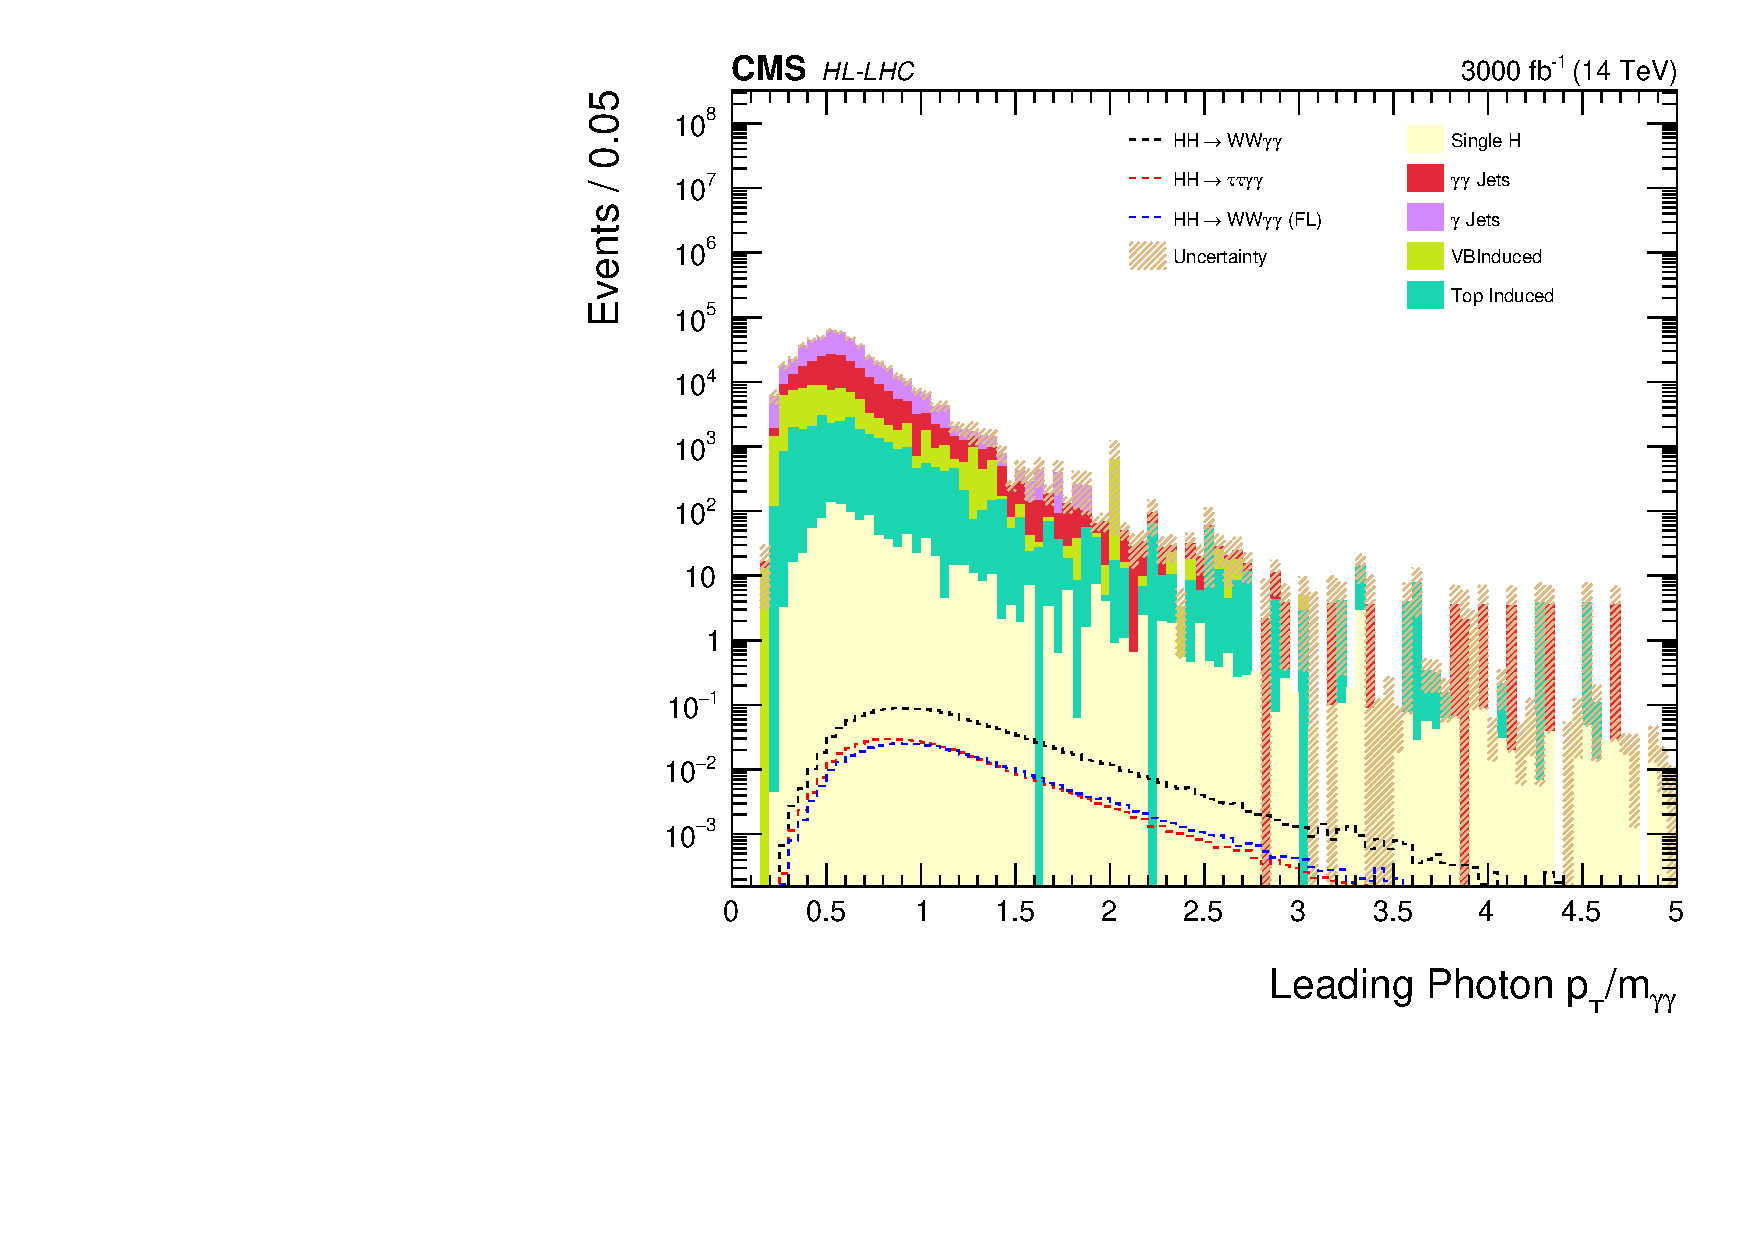
\includegraphics[width=\textwidth]{c3_pt_mgg_logy.pdf}
        \vspace{-0.5cm}
        \firstsubcaption{Leading Photon $p_{T}/m_{\gamma\gamma}$}
    \end{subfigure}
    \hfill
    \begin{subfigure}[b]{0.475\textwidth}  
        \centering 
        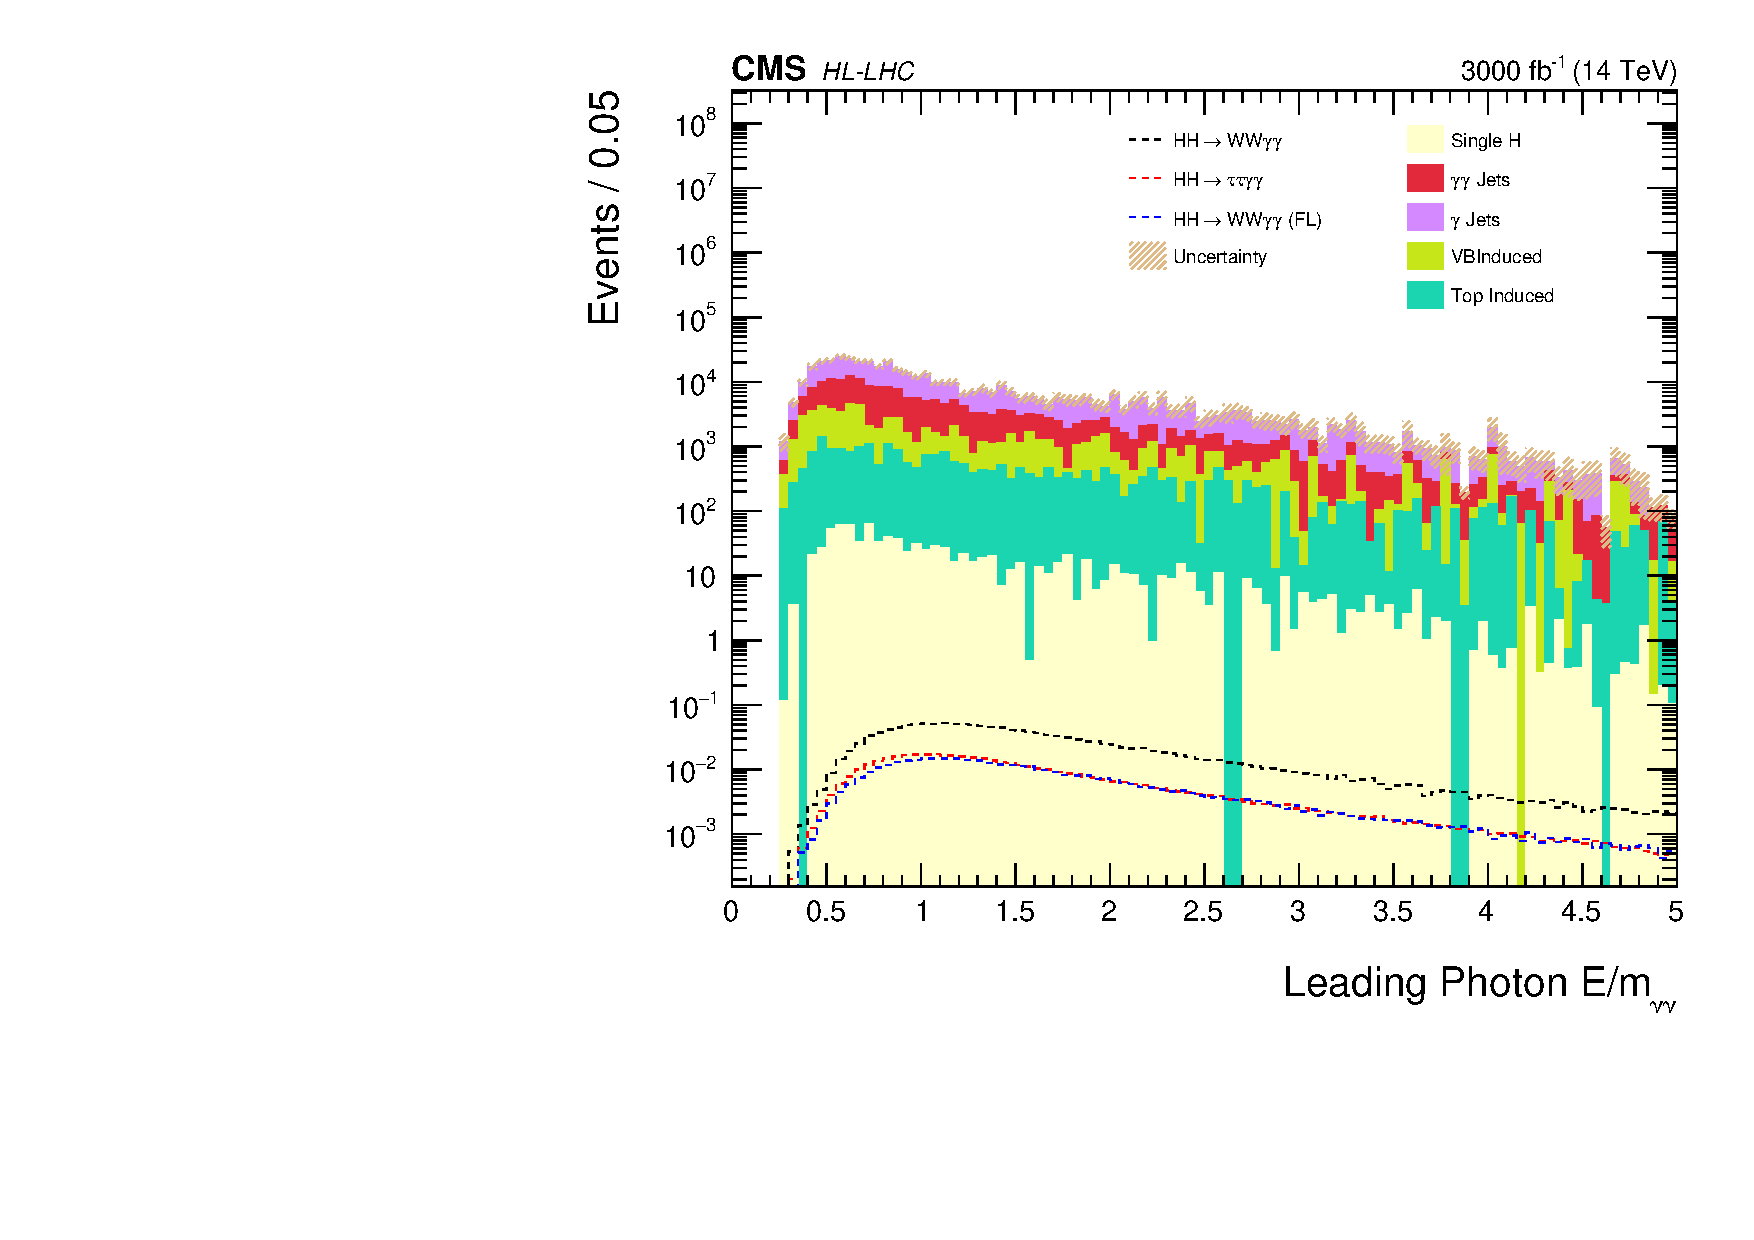
\includegraphics[width=\textwidth]{c3_LE_mgg_logy.pdf}
        \vspace{-0.5cm}
        \firstsubcaption{Leading Photon $E/m_{\gamma\gamma}$}
    \end{subfigure}
    \vskip\baselineskip
    \begin{subfigure}[b]{0.475\textwidth}   
        \centering 
        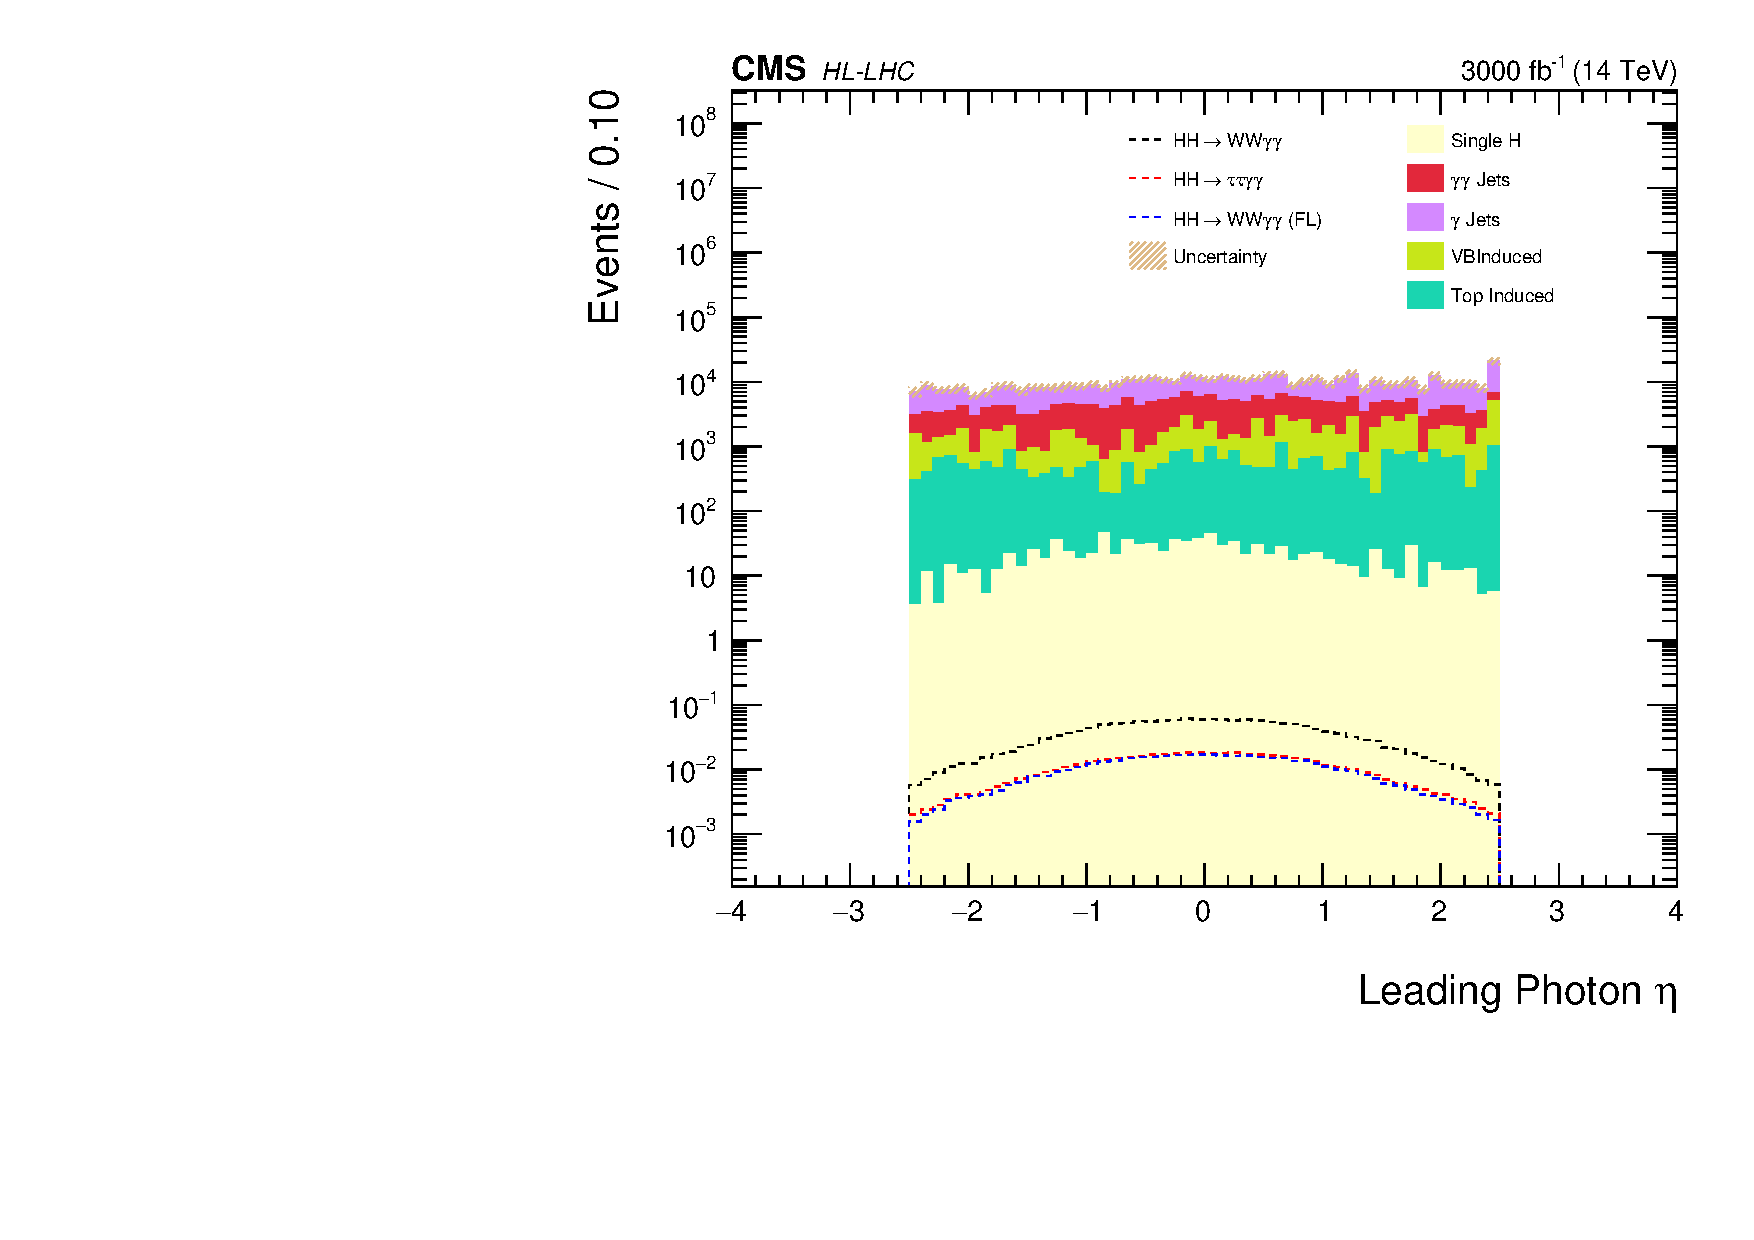
\includegraphics[width=\textwidth]{c3_leadingphoton_eta_logy.pdf}
        \vspace{-0.5cm}
        \firstsubcaption{Leading Photon $\eta$}
    \end{subfigure}
    \hfill
    \begin{subfigure}[b]{0.475\textwidth}   
        \centering 
        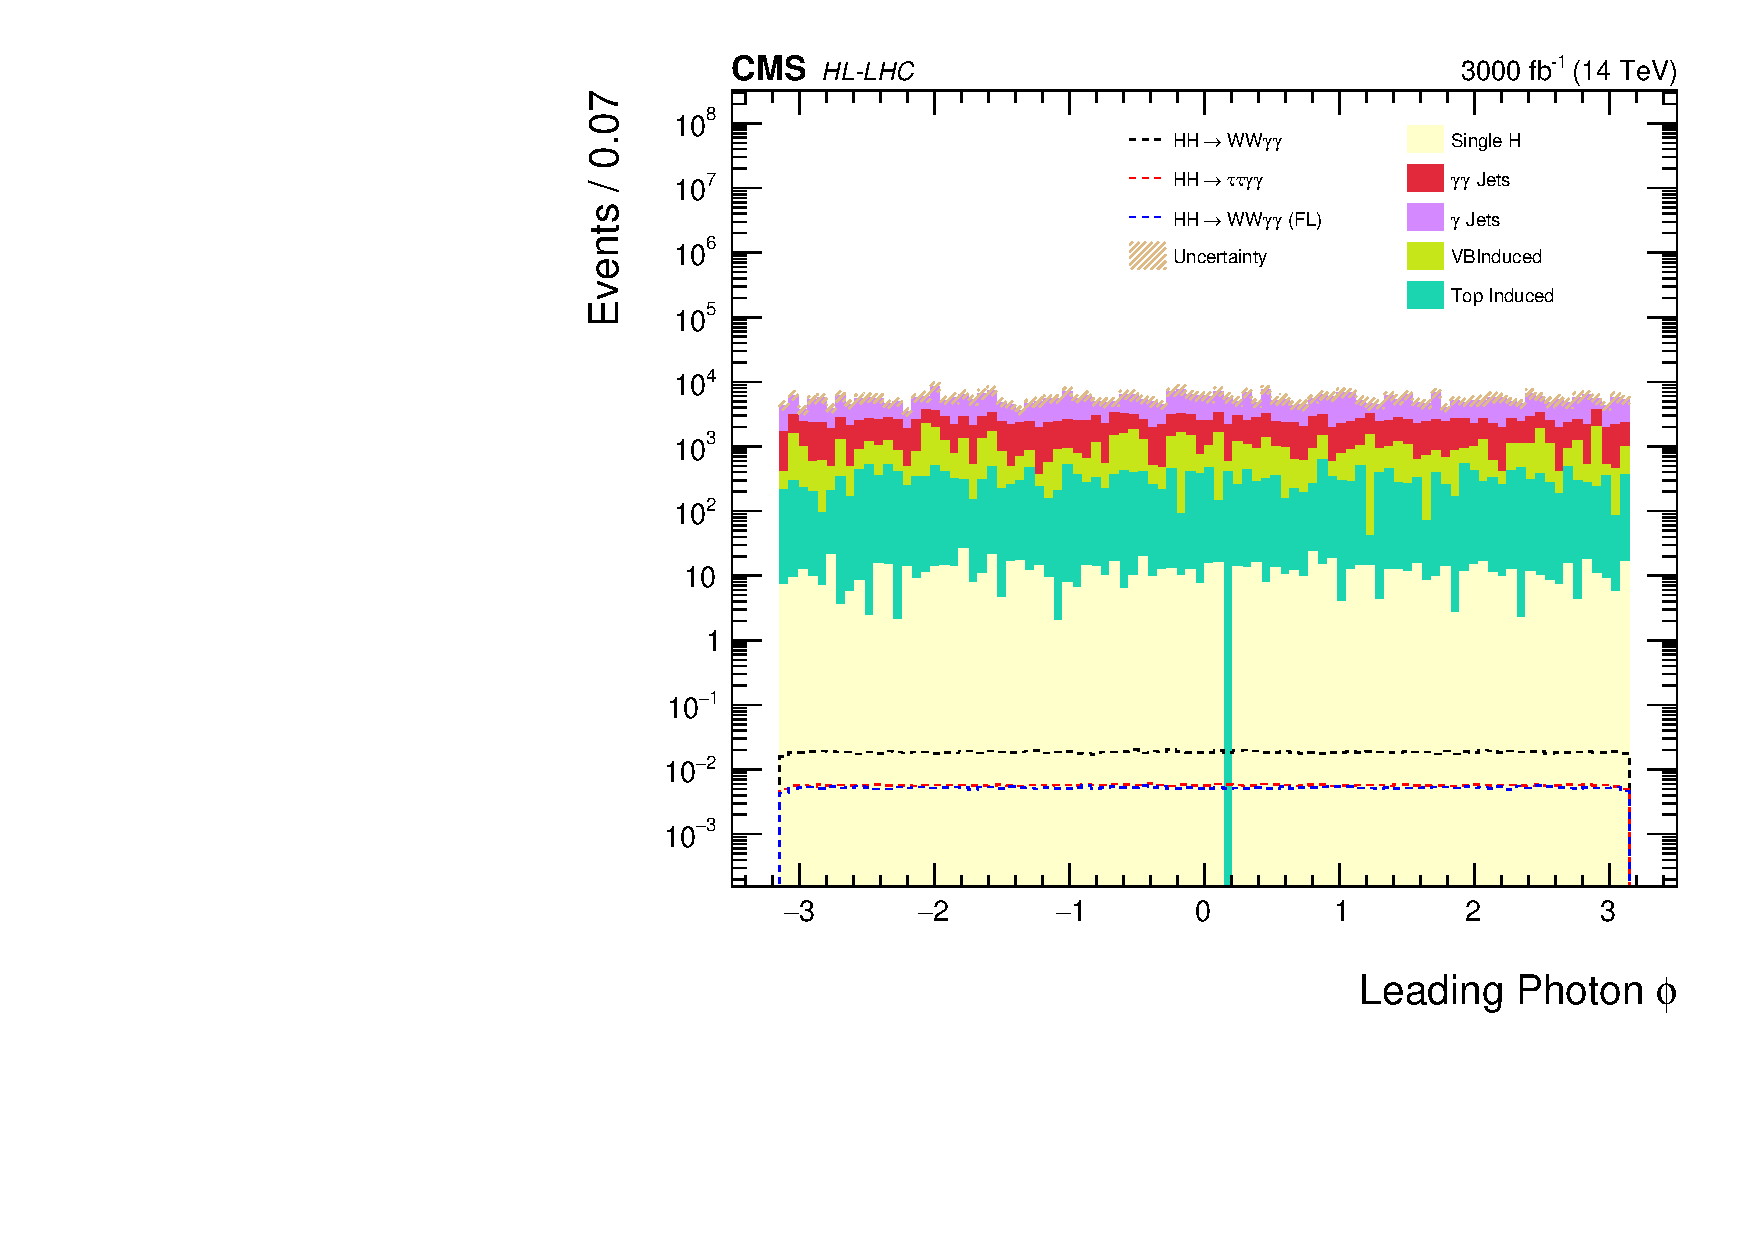
\includegraphics[width=\textwidth]{c3_leadingphoton_phi_logy.pdf}
        \vspace{-0.5cm}
        \firstsubcaption{Leading Photon $\phi$}
    \end{subfigure}
    \vskip\baselineskip
    \begin{subfigure}[b]{0.475\textwidth}   
        \centering 
        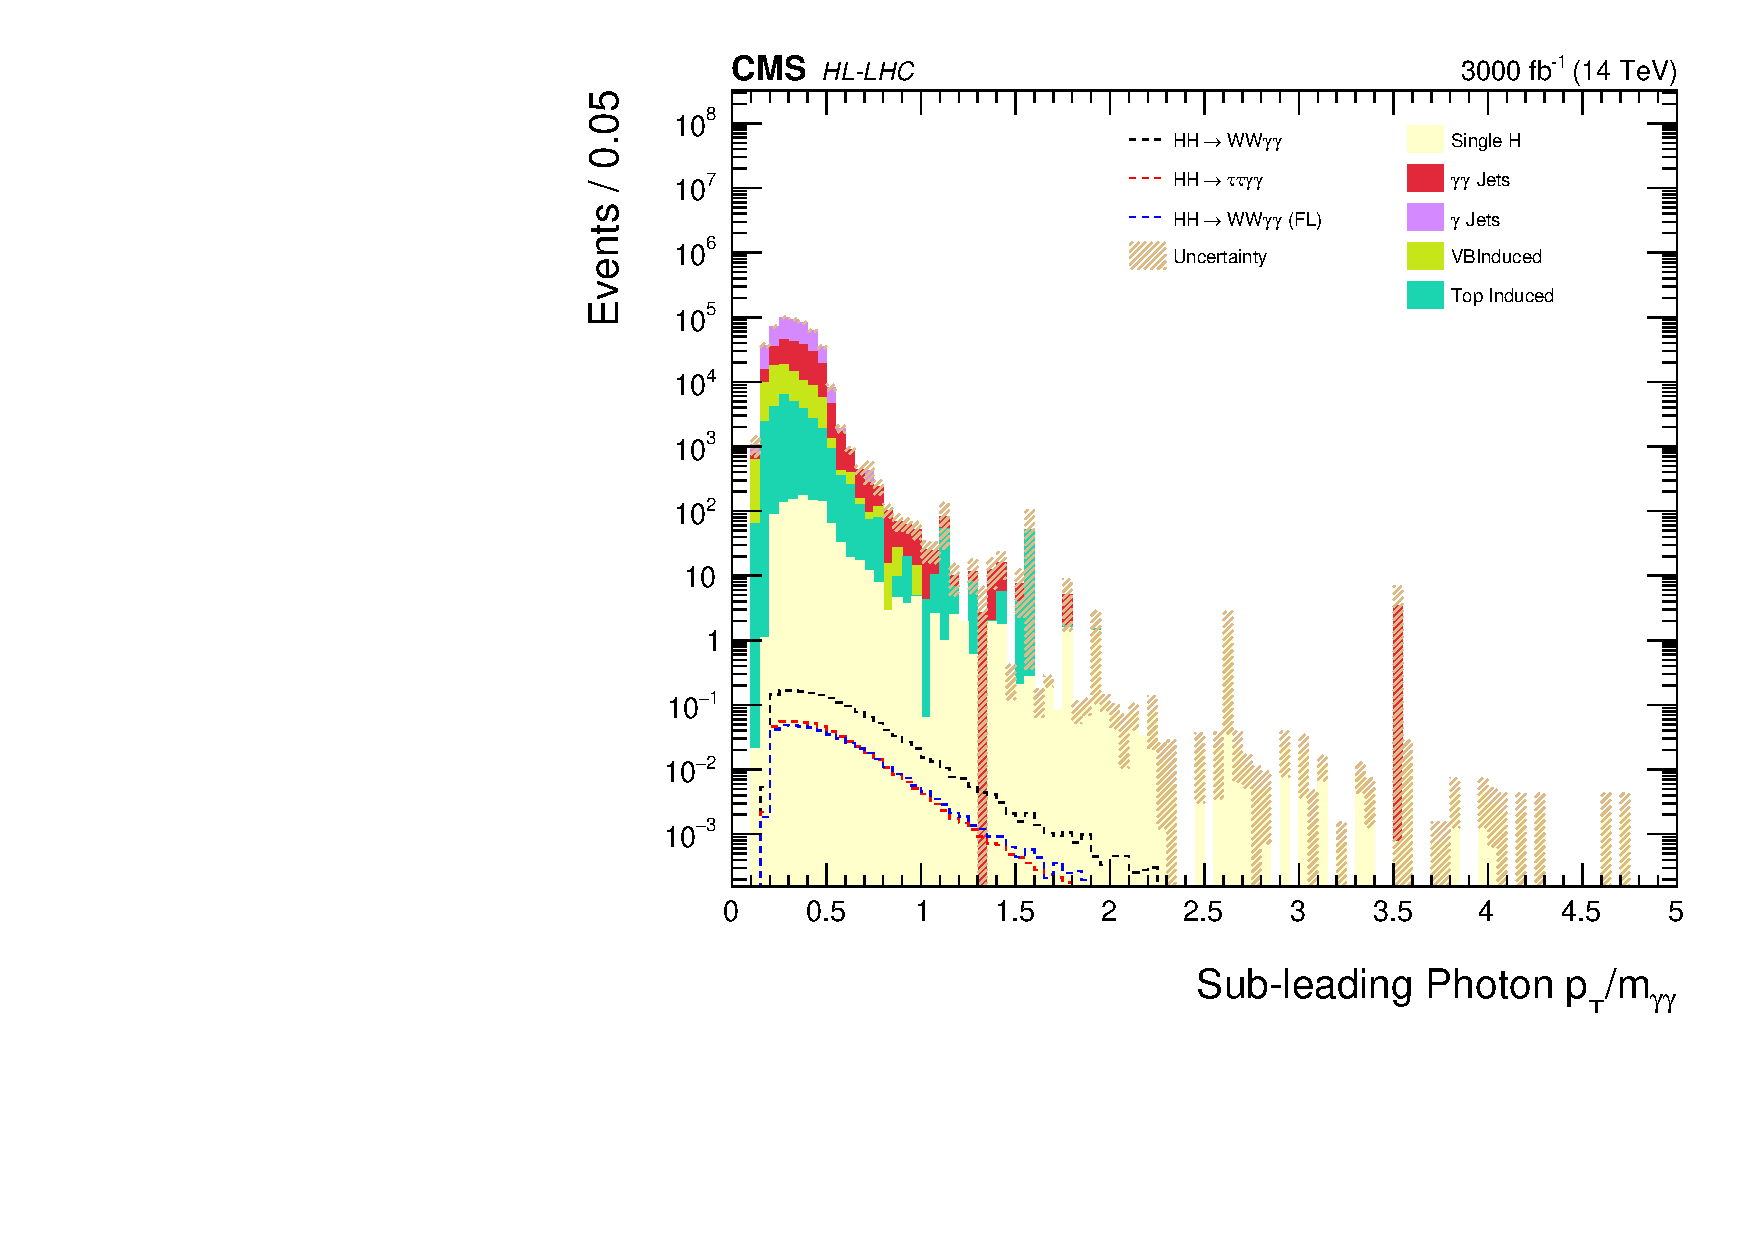
\includegraphics[width=\textwidth]{c3_SLpt_mgg_logy.pdf}
        \vspace{-0.5cm}
        \firstsubcaption{Sub-leading Photon $p_{T}/m_{\gamma\gamma}$}
    \end{subfigure}
    \hfill
    \begin{subfigure}[b]{0.475\textwidth}   
        \centering 
        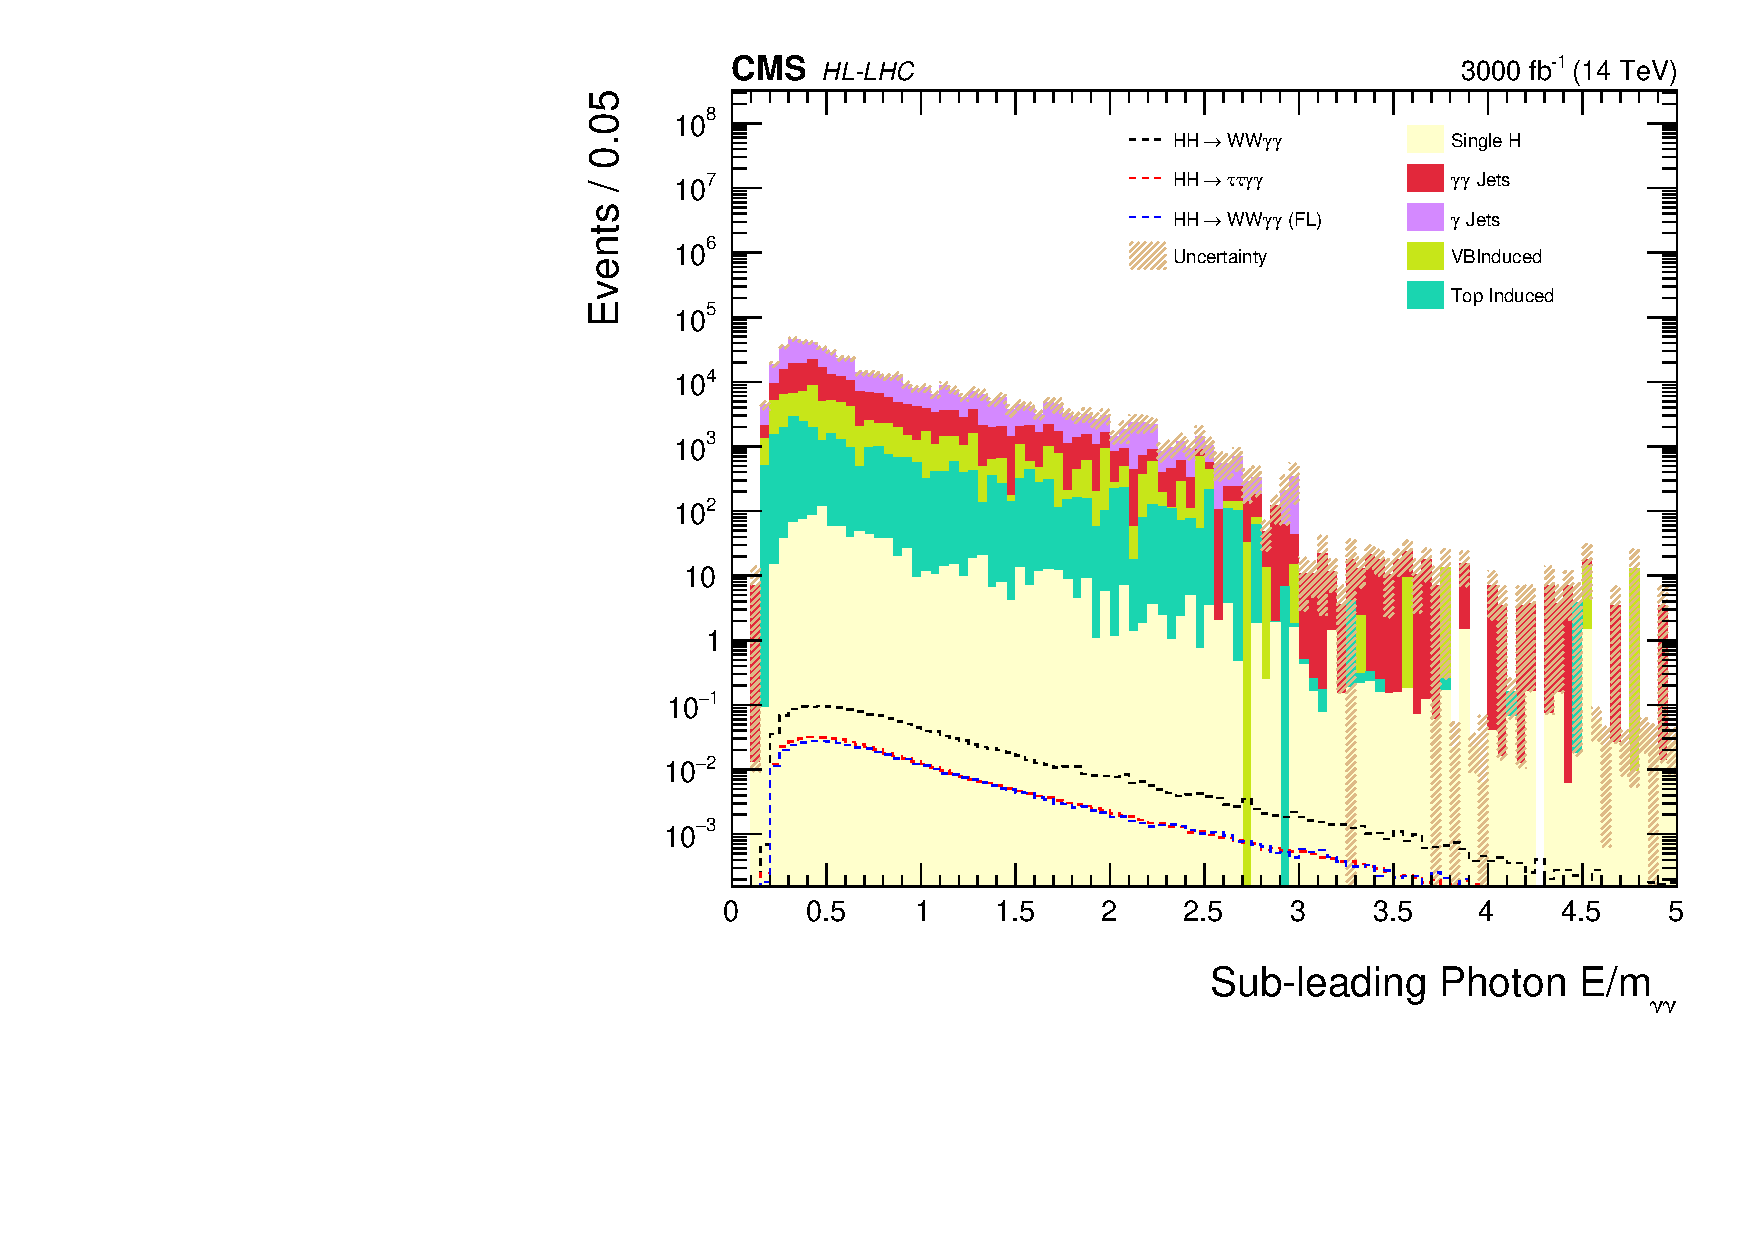
\includegraphics[width=\textwidth]{c3_SLE_mgg_logy.pdf}
        \vspace{-0.5cm}
        \firstsubcaption{Sub-leading Photon $E/m_{\gamma\gamma}$}   
    \end{subfigure}
    \caption{\small DNN input distributions for the 1$\tau$ channel of $HH\rightarrow{\tau\tau\gamma\gamma}$ (continued).}
    \label{dnninputDists_tau}
\end{figure*}

\begin{figure*}[h!]
    \centering
    \begin{subfigure}[b]{0.475\textwidth}
        \centering
        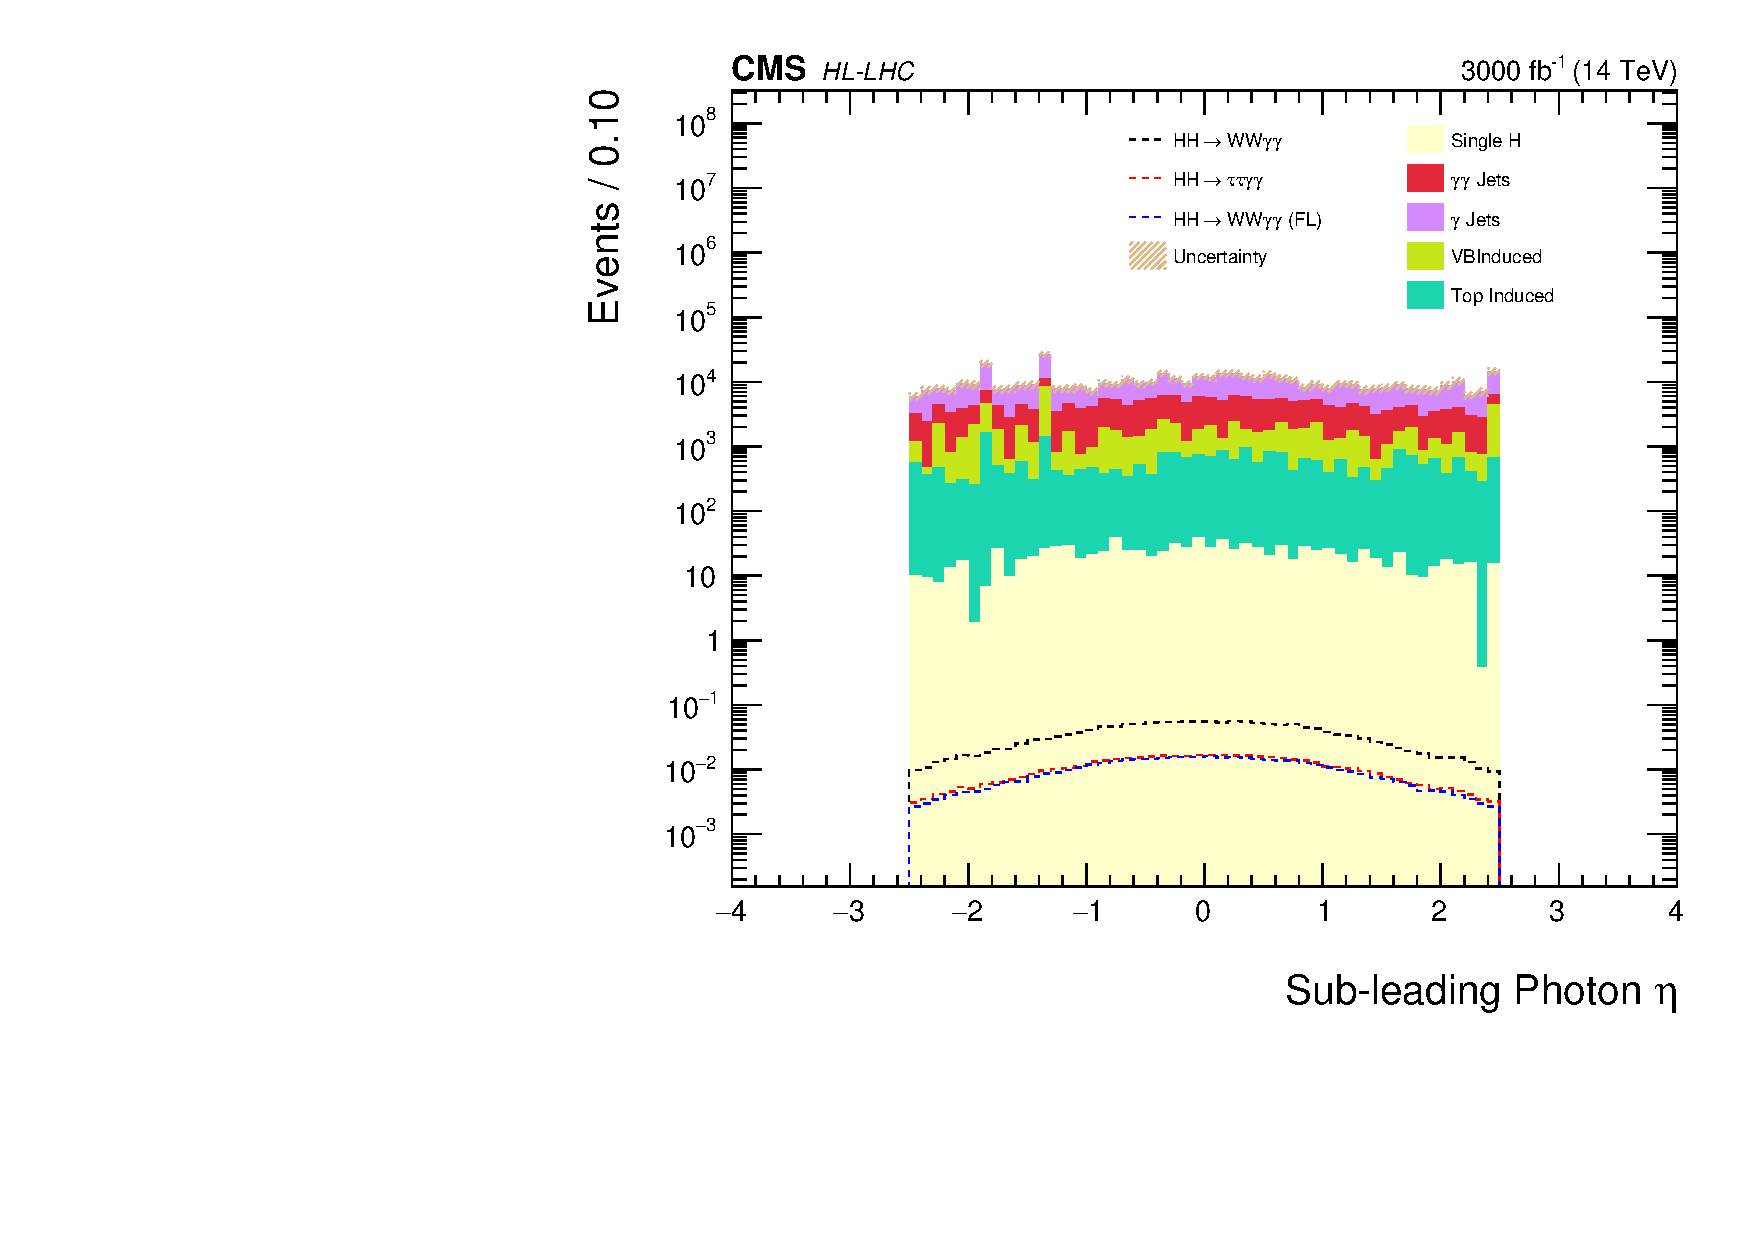
\includegraphics[width=\textwidth]{c3_subleadingphoton_eta_logy.pdf}
        \vspace{-0.5cm}
        \firstsubcaption{Sub-leading Photon $\eta$}
    \end{subfigure}
    \hfill
    \begin{subfigure}[b]{0.475\textwidth}  
        \centering 
        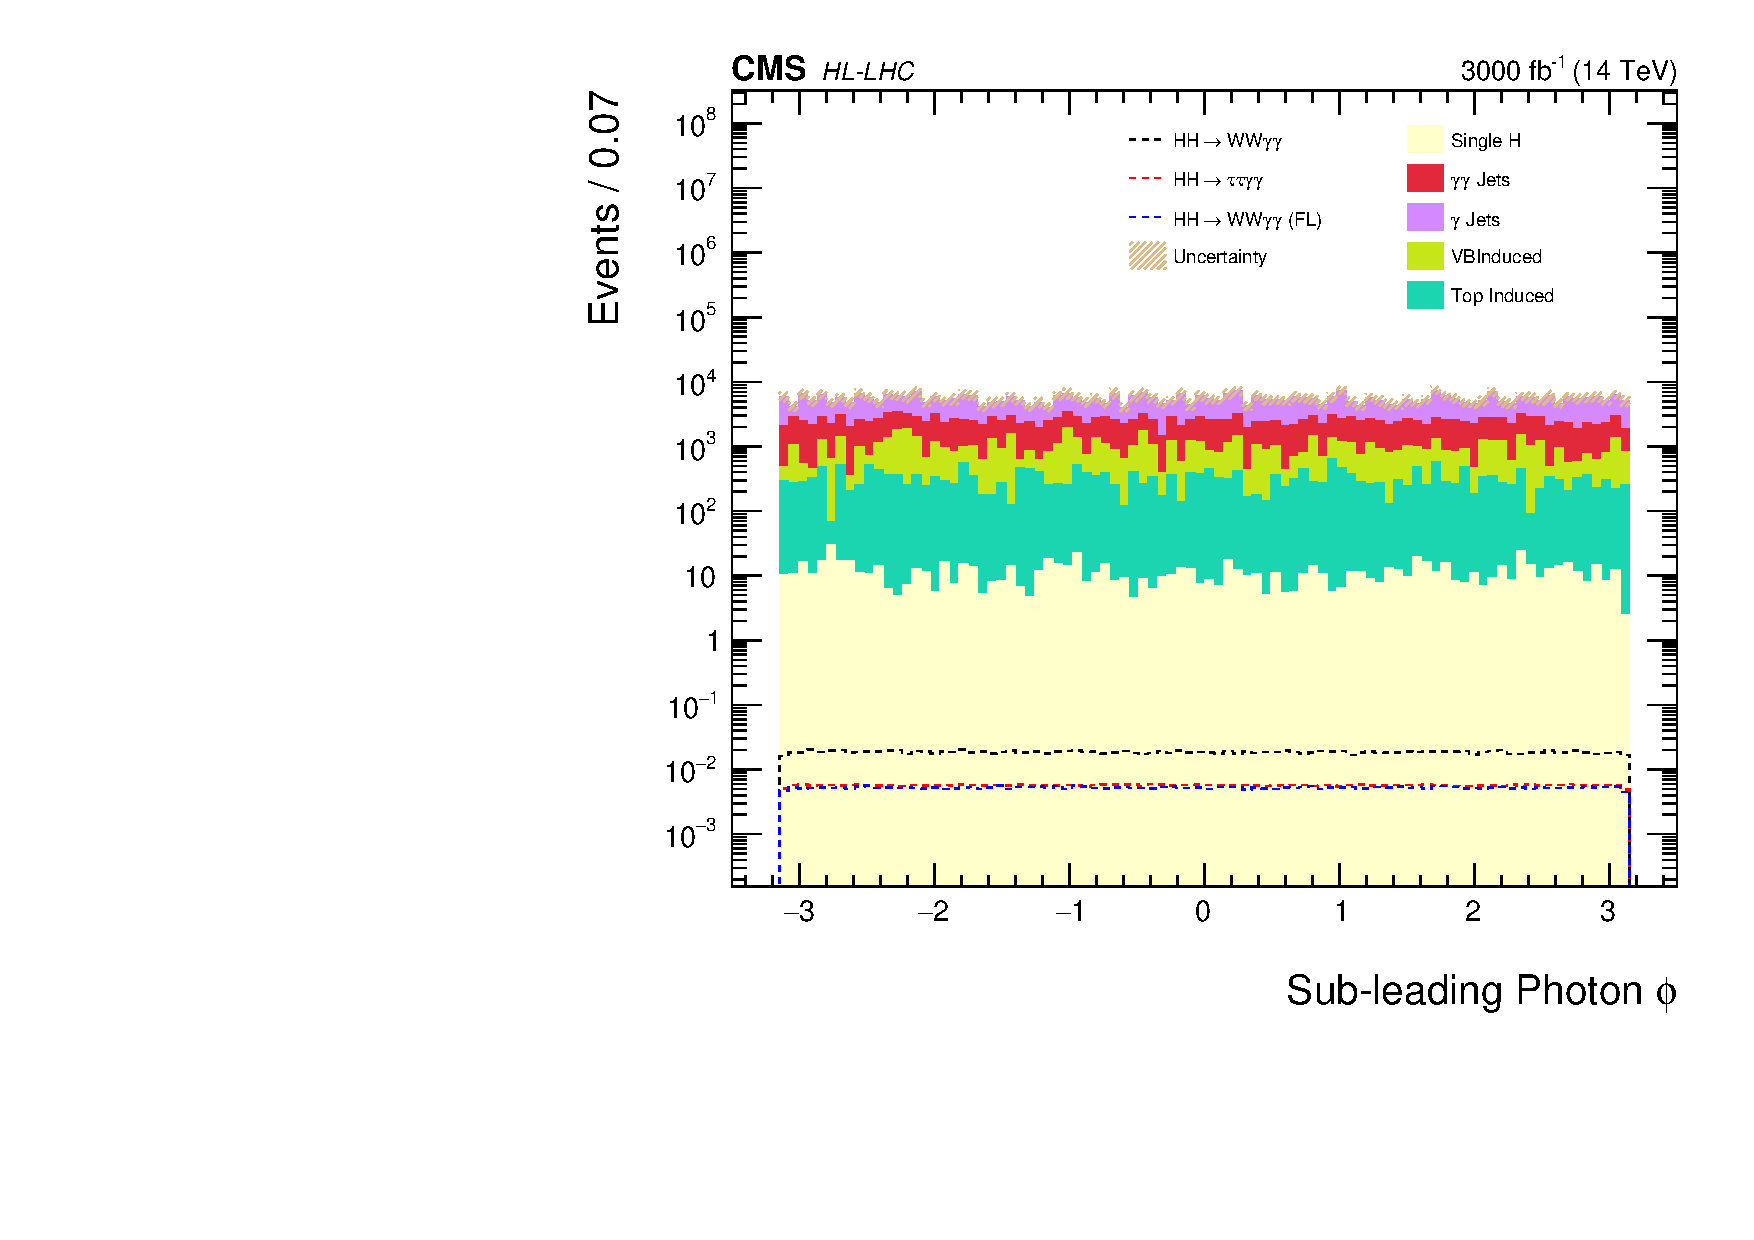
\includegraphics[width=\textwidth]{c3_subleadingphoton_phi_logy.pdf}
        \vspace{-0.5cm}
        \firstsubcaption{Sub-leading Photon $\phi$}
    \end{subfigure}
    \vskip\baselineskip
    \begin{subfigure}[b]{0.475\textwidth}   
        \centering 
        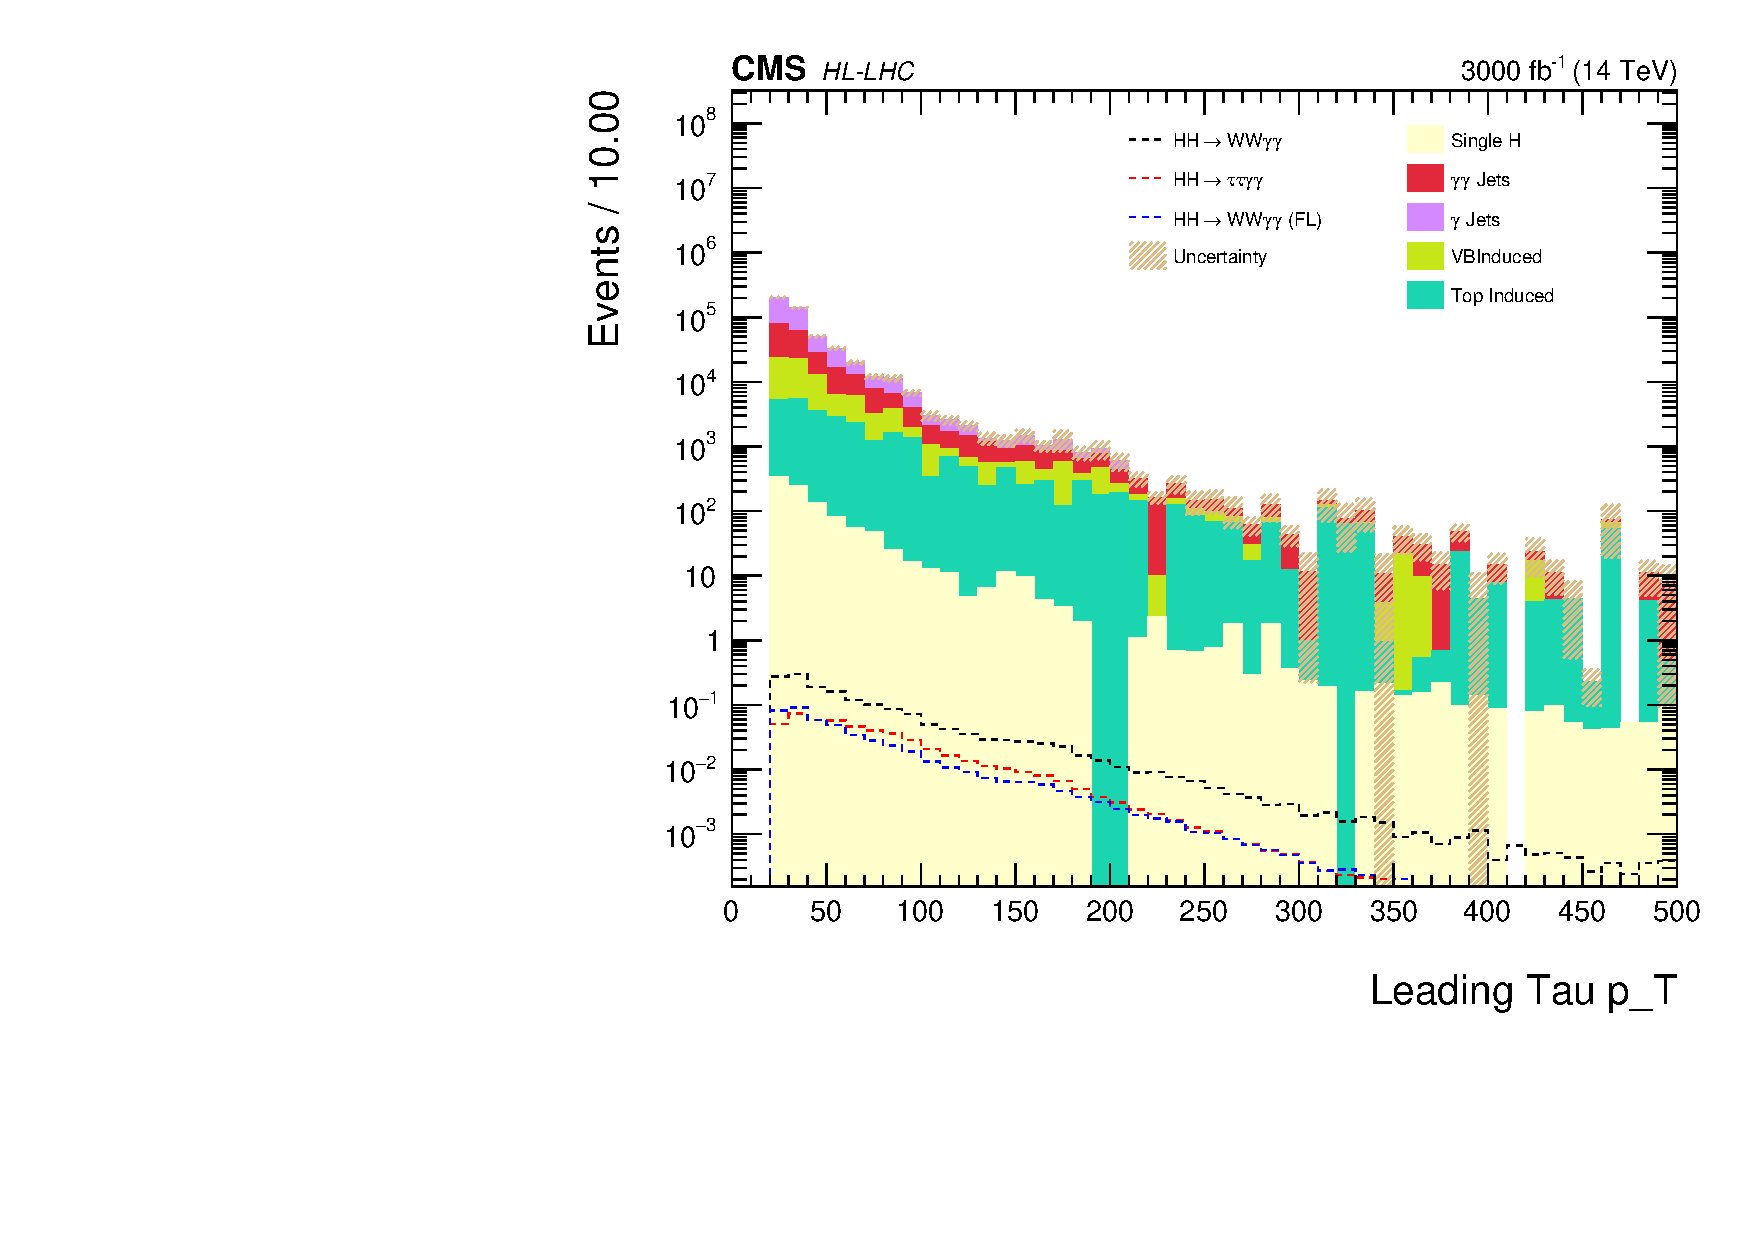
\includegraphics[width=\textwidth]{c3_leadingtau_pt_logy.pdf}
        \vspace{-0.5cm}
        \firstsubcaption{Leading Tau \pt}
    \end{subfigure}
    \hfill
    \begin{subfigure}[b]{0.475\textwidth}   
        \centering 
        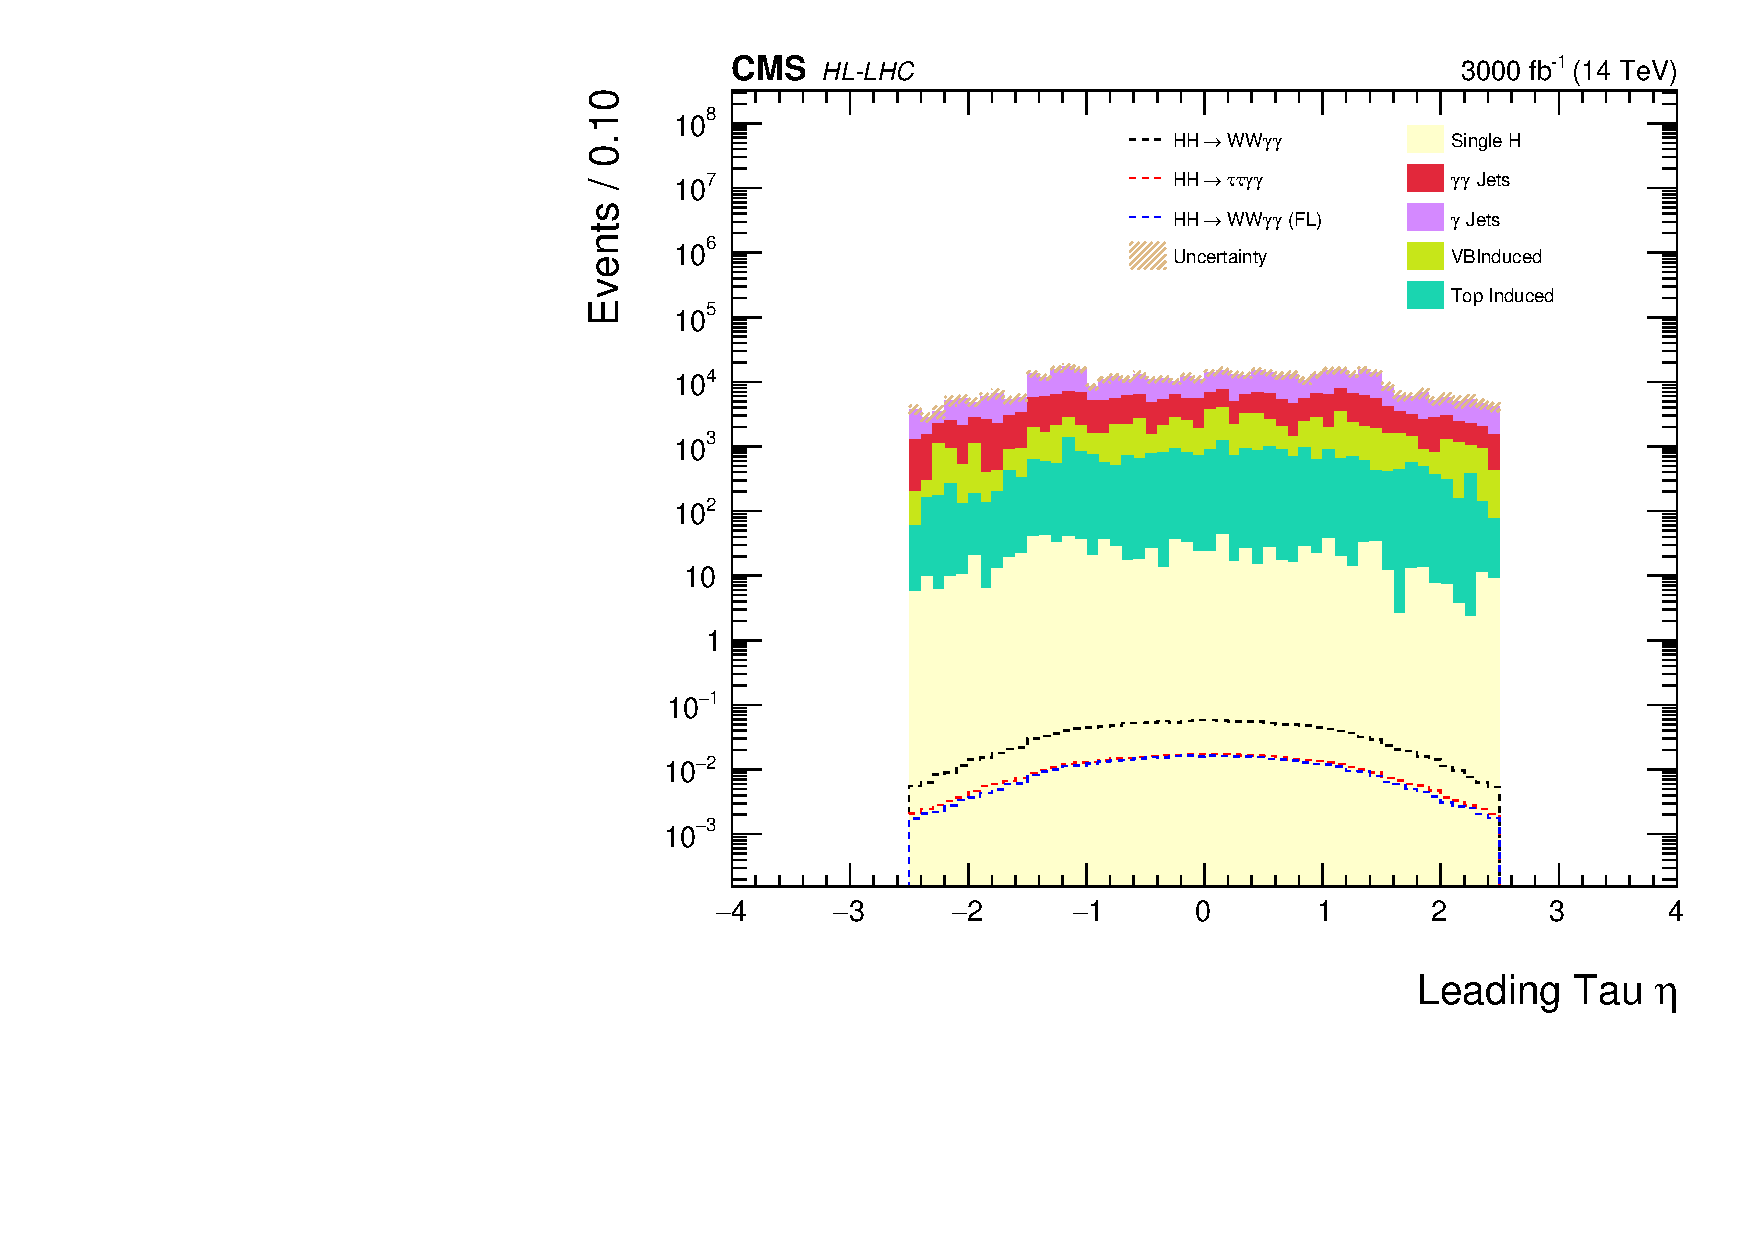
\includegraphics[width=\textwidth]{c3_leadingtau_eta_logy.pdf}
        \vspace{-0.5cm}
        \firstsubcaption{Leading Tau $\eta$}
    \end{subfigure}
    \vskip\baselineskip
    \begin{subfigure}[b]{0.475\textwidth}   
        \centering 
        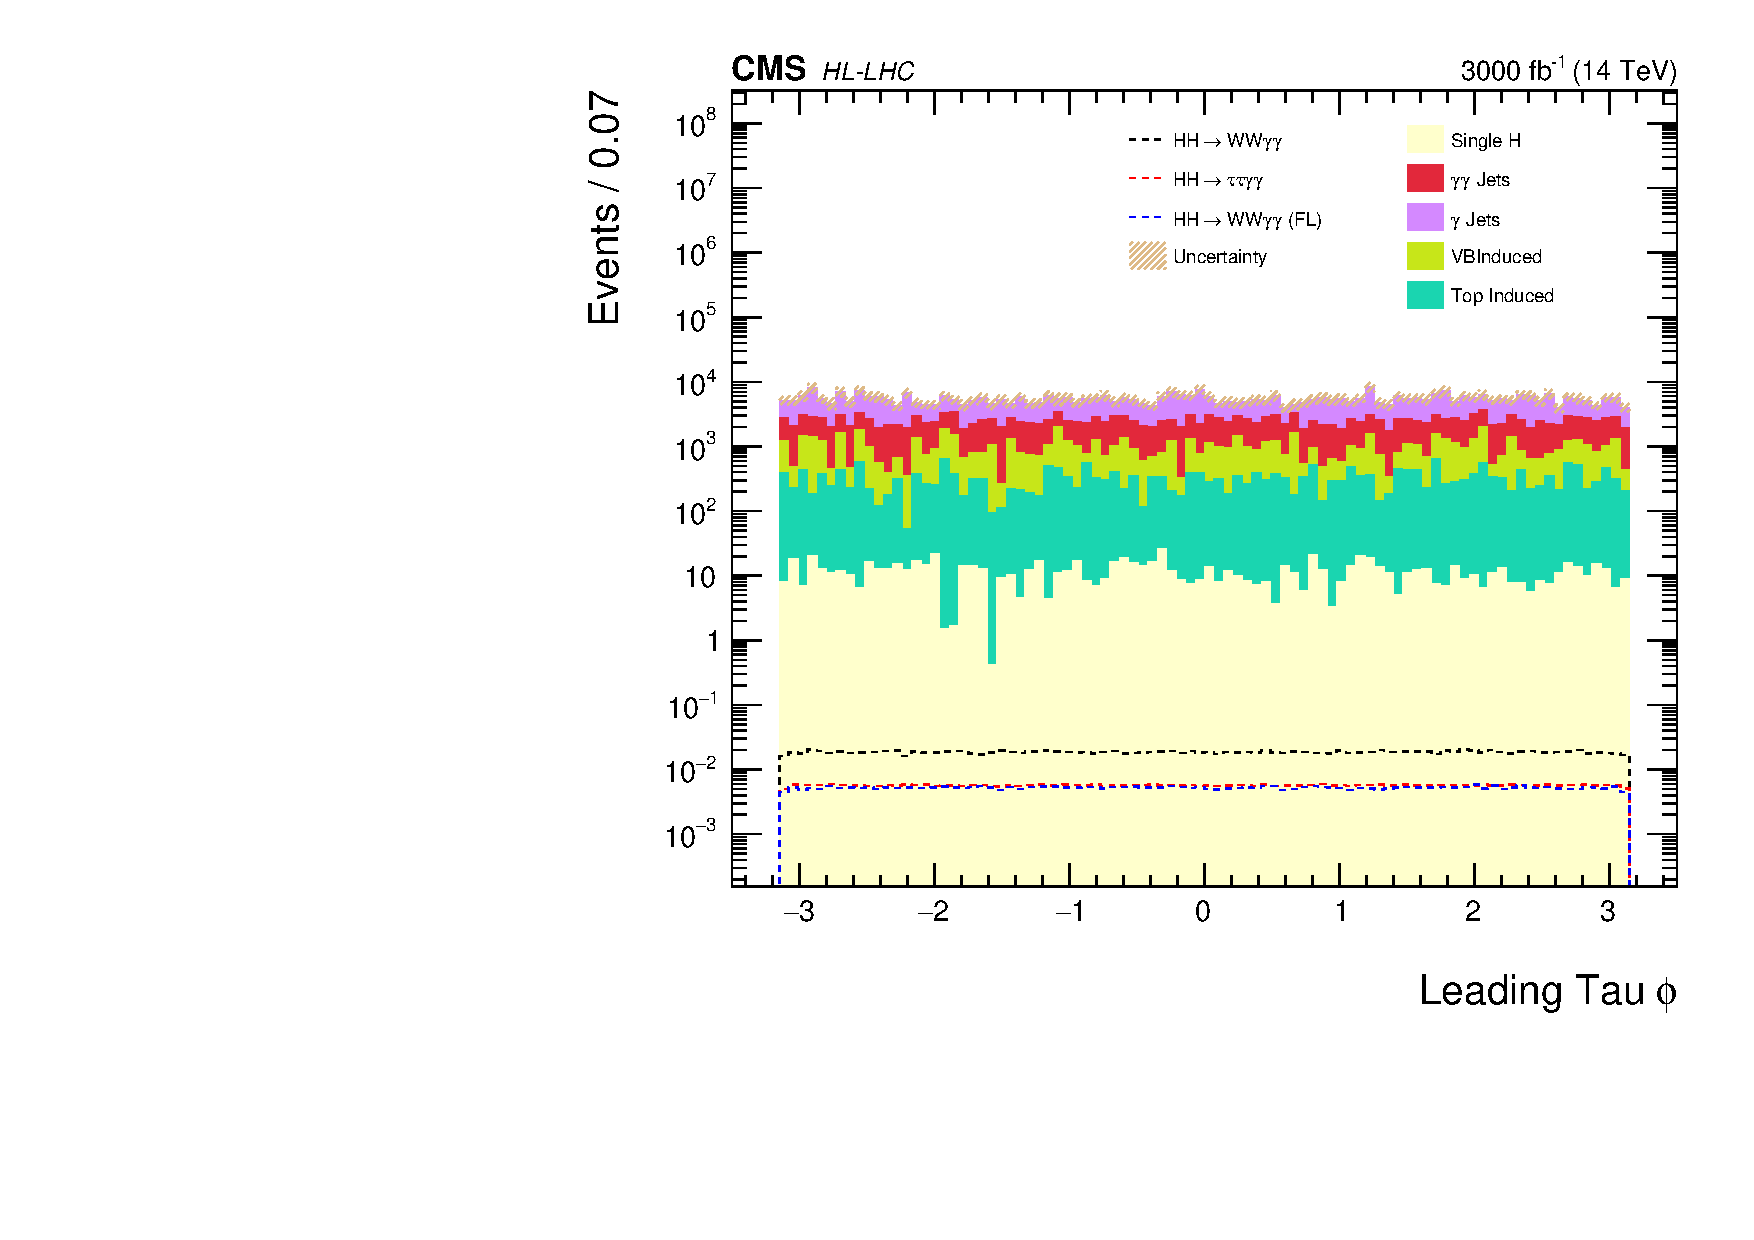
\includegraphics[width=\textwidth]{c3_leadingtau_phi_logy.pdf}
        \vspace{-0.5cm}
        \firstsubcaption{Leading Tau $\phi$}
    \end{subfigure}
    \hfill
    \begin{subfigure}[b]{0.475\textwidth}   
        \centering 
        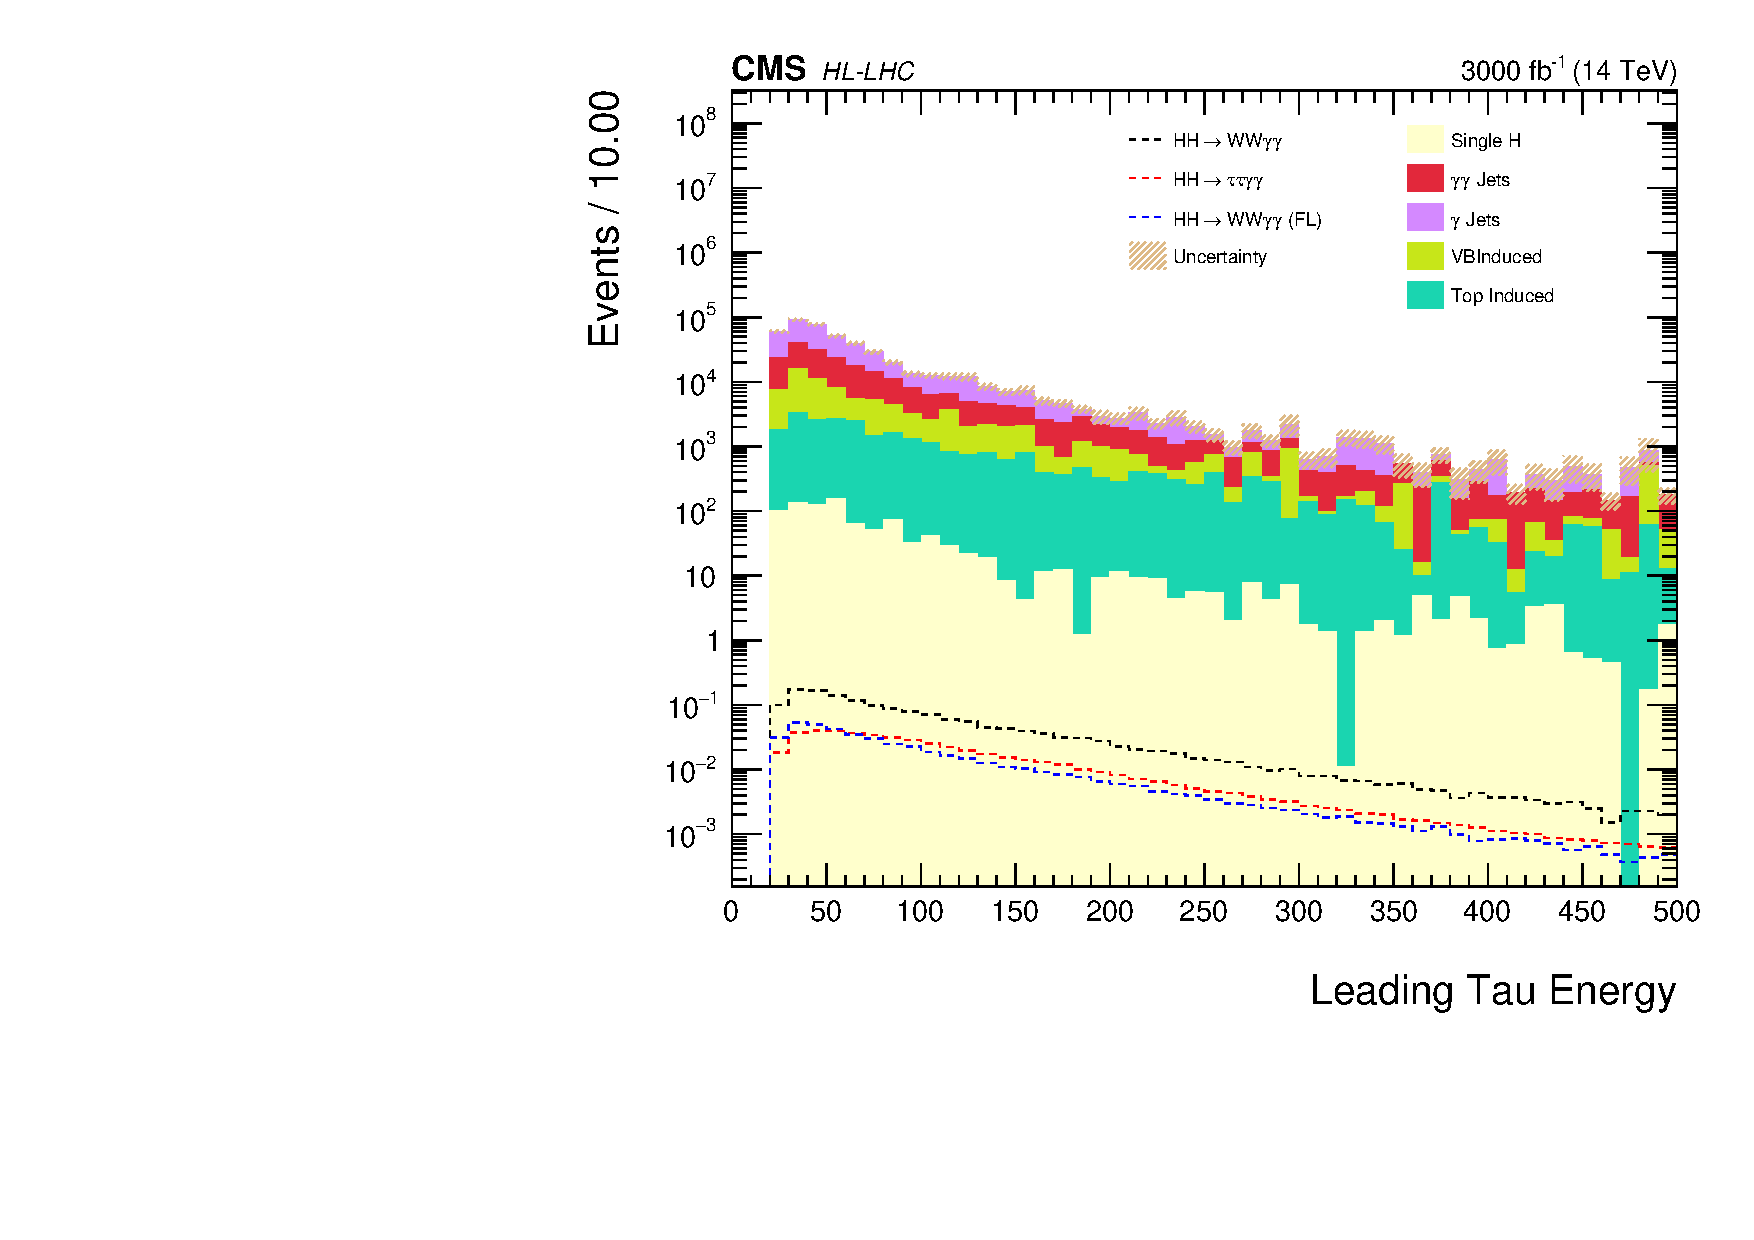
\includegraphics[width=\textwidth]{c3_leadingtau_E_logy.pdf}
        \vspace{-0.5cm}
        \firstsubcaption{Leading Tau energy}   
    \end{subfigure}
    \caption{\small DNN input distributions for the 1$\tau$ channel of $HH\rightarrow{\tau\tau\gamma\gamma}$ (continued).}
\end{figure*}


\begin{figure*}[h!]
    \centering
    \begin{subfigure}[b]{0.475\textwidth}
        \centering
        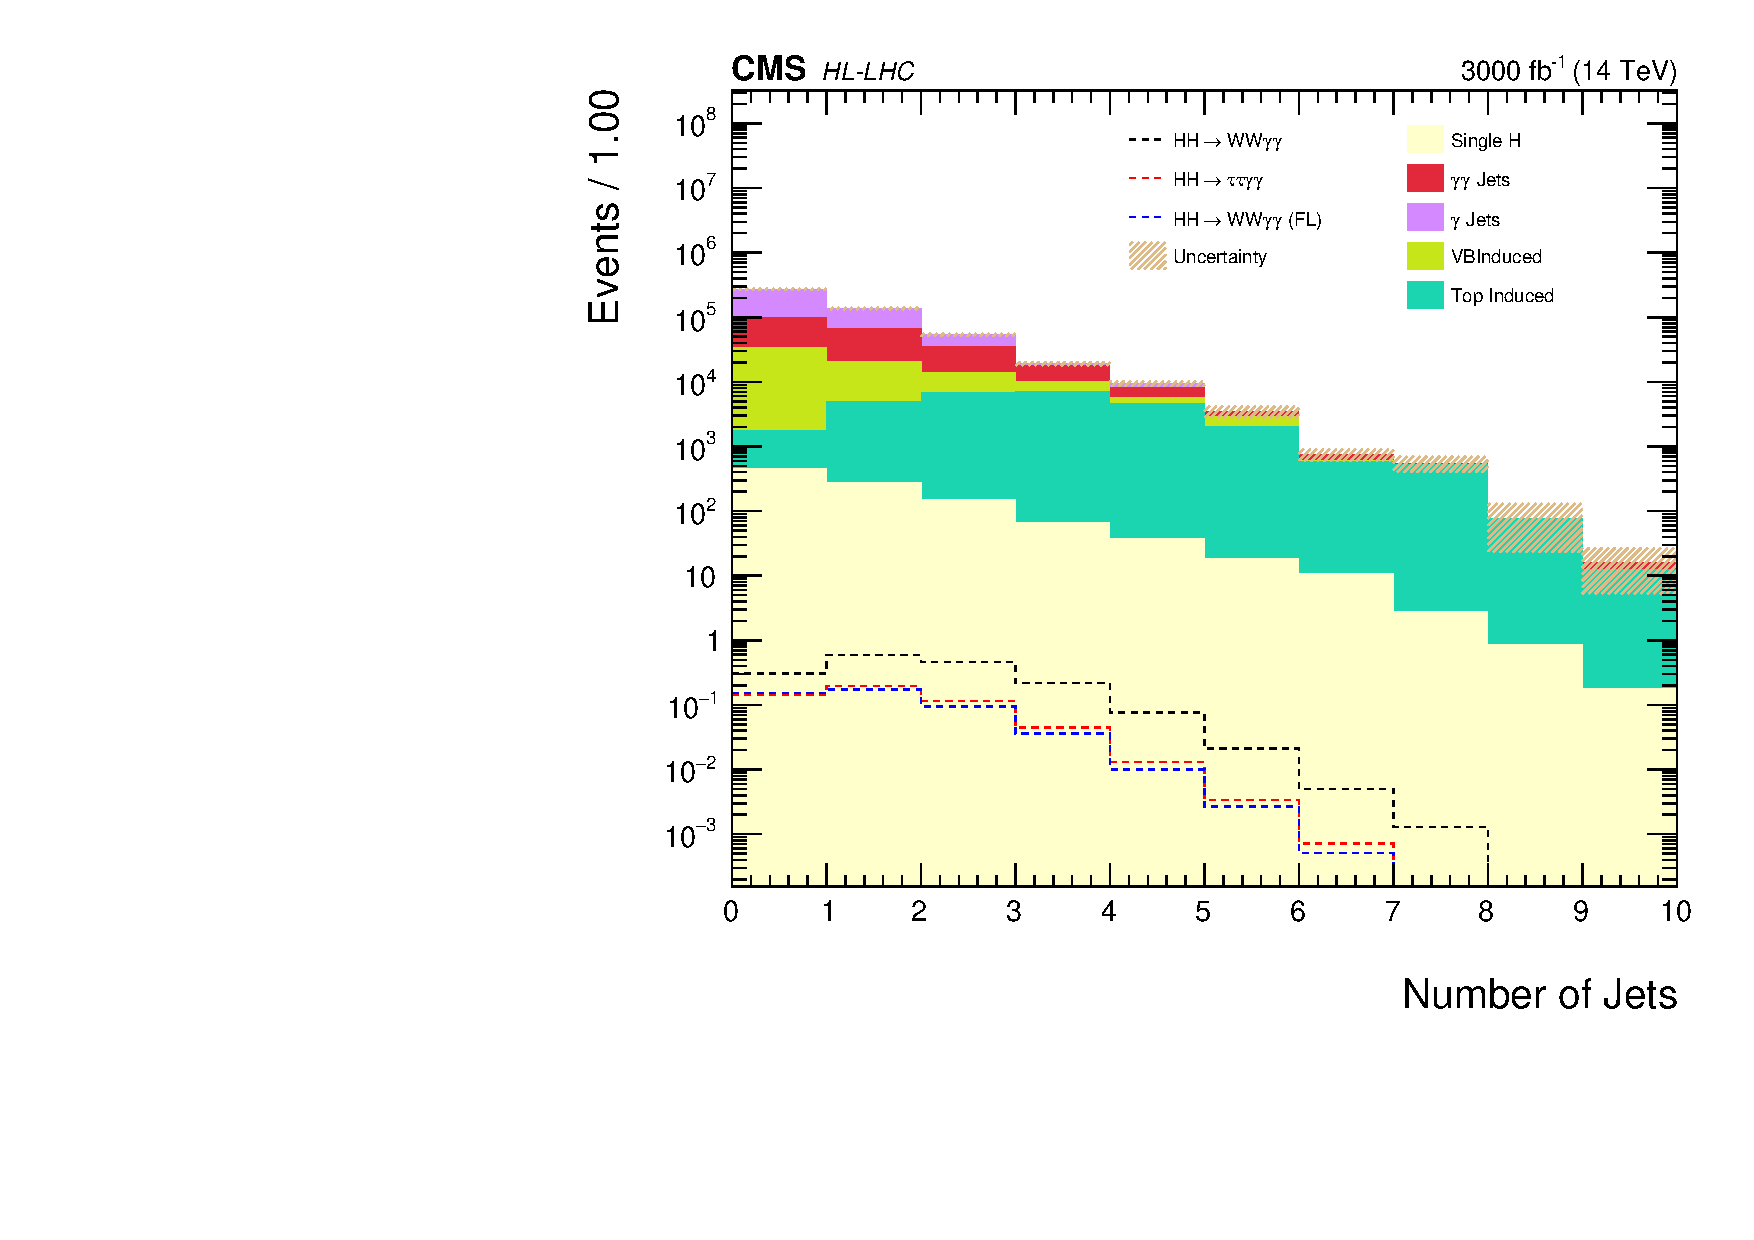
\includegraphics[width=\textwidth]{c3_nJet_logy.pdf}
        \vspace{-0.5cm}
        \firstsubcaption{Jet multiplicity}
    \end{subfigure}
    \hfill
    \begin{subfigure}[b]{0.475\textwidth}  
        \centering 
        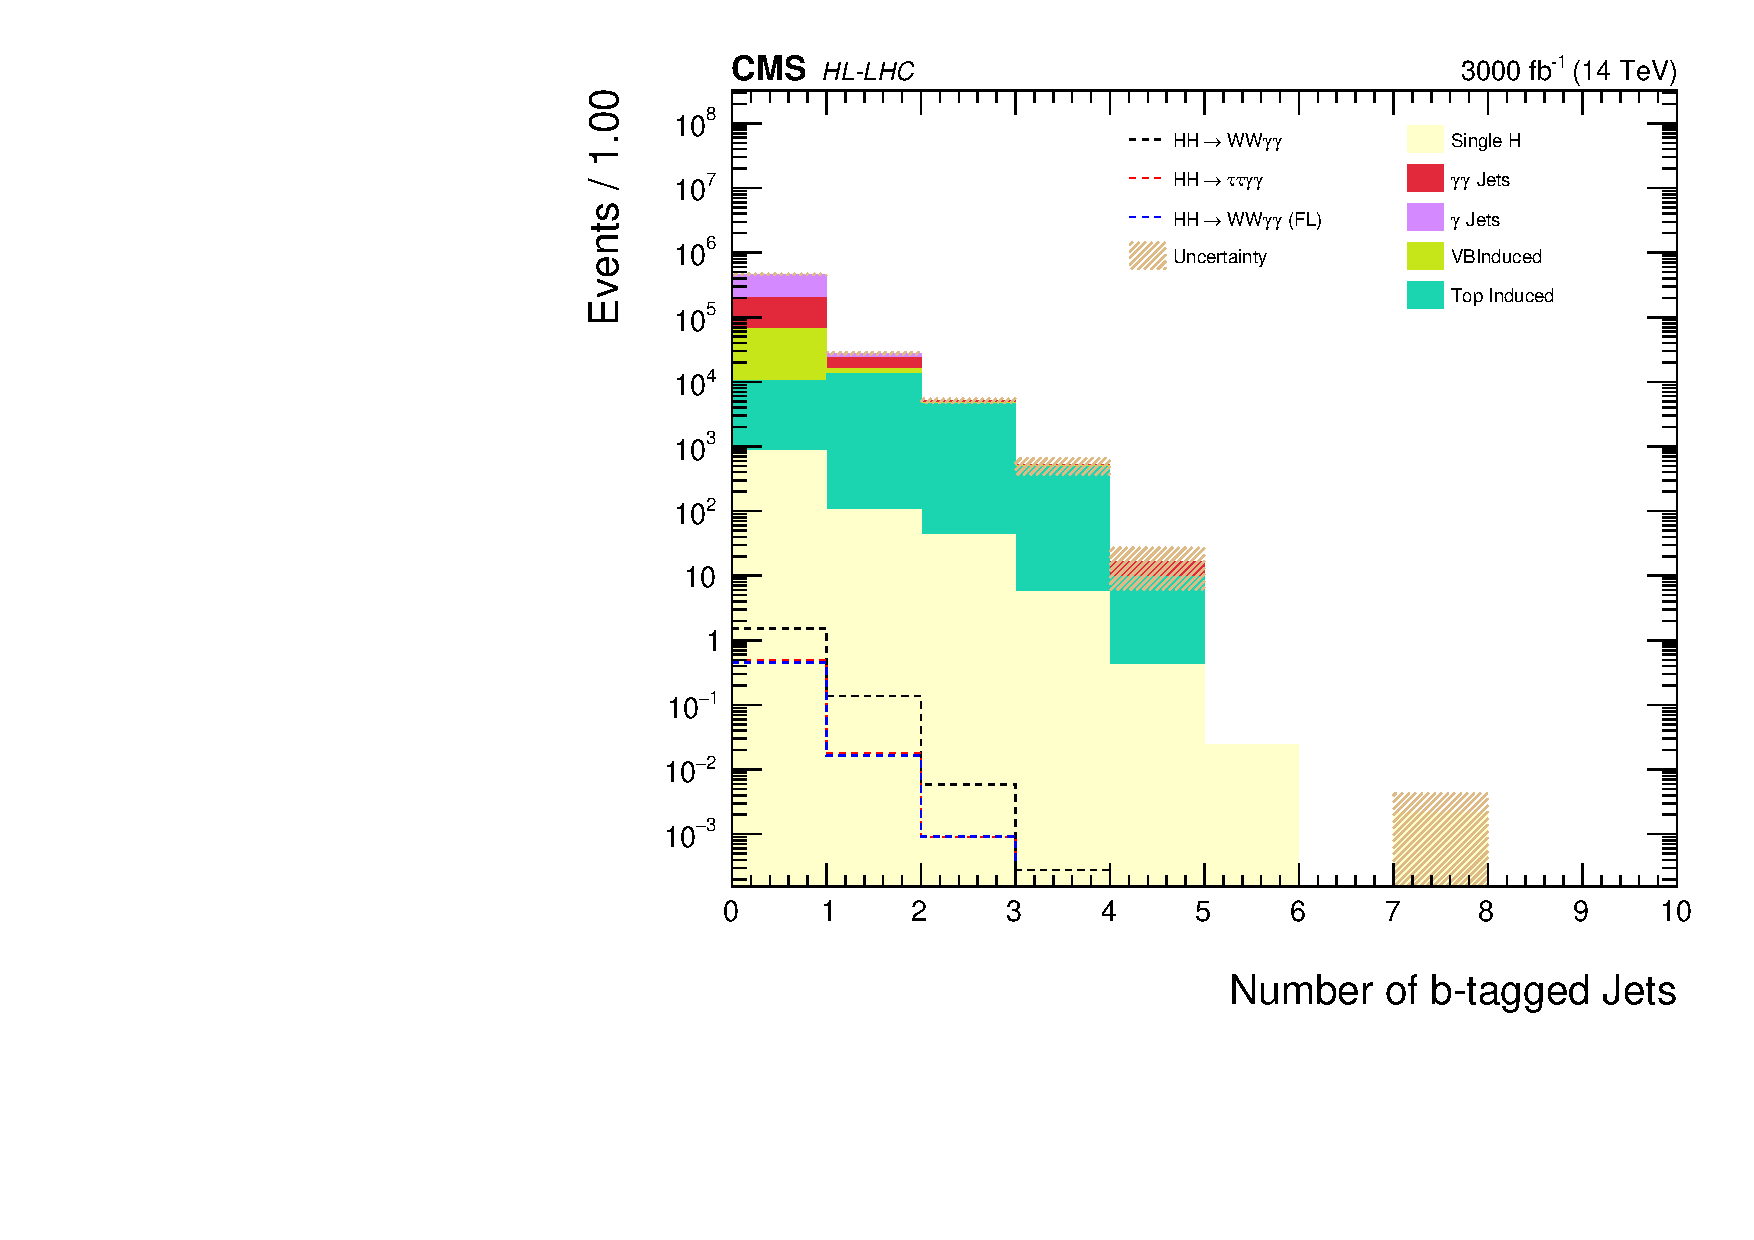
\includegraphics[width=\textwidth]{c3_nbJet_logy.pdf}
        \vspace{-0.5cm}
        \firstsubcaption{B-tagged jet multiplicity}
    \end{subfigure}
    \vskip\baselineskip
    \begin{subfigure}[b]{0.475\textwidth}   
        \centering 
        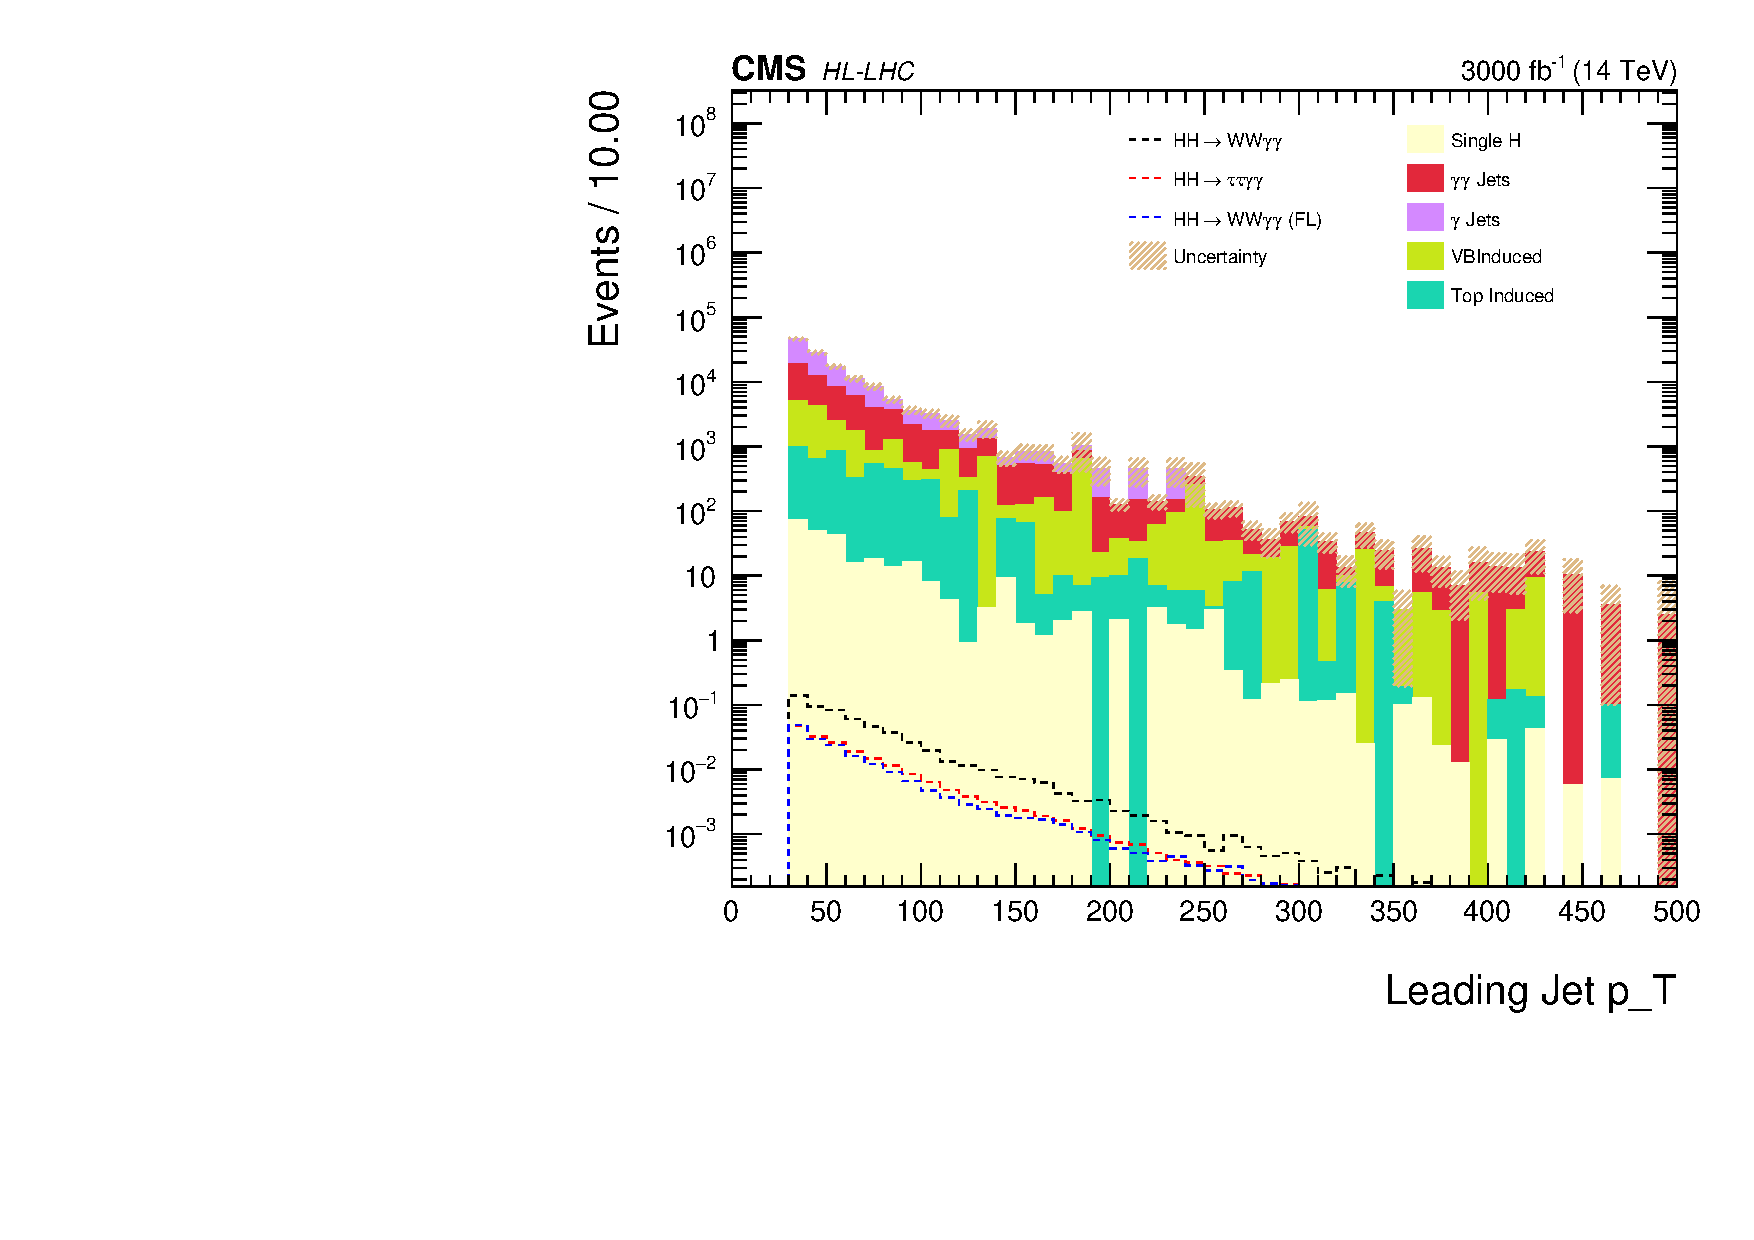
\includegraphics[width=\textwidth]{c3_oneJet_Ljetpt_logy.pdf}
        \vspace{-0.5cm}
        \firstsubcaption{Leading jet \pt}
    \end{subfigure}
    \hfill
    \begin{subfigure}[b]{0.475\textwidth}   
        \centering 
        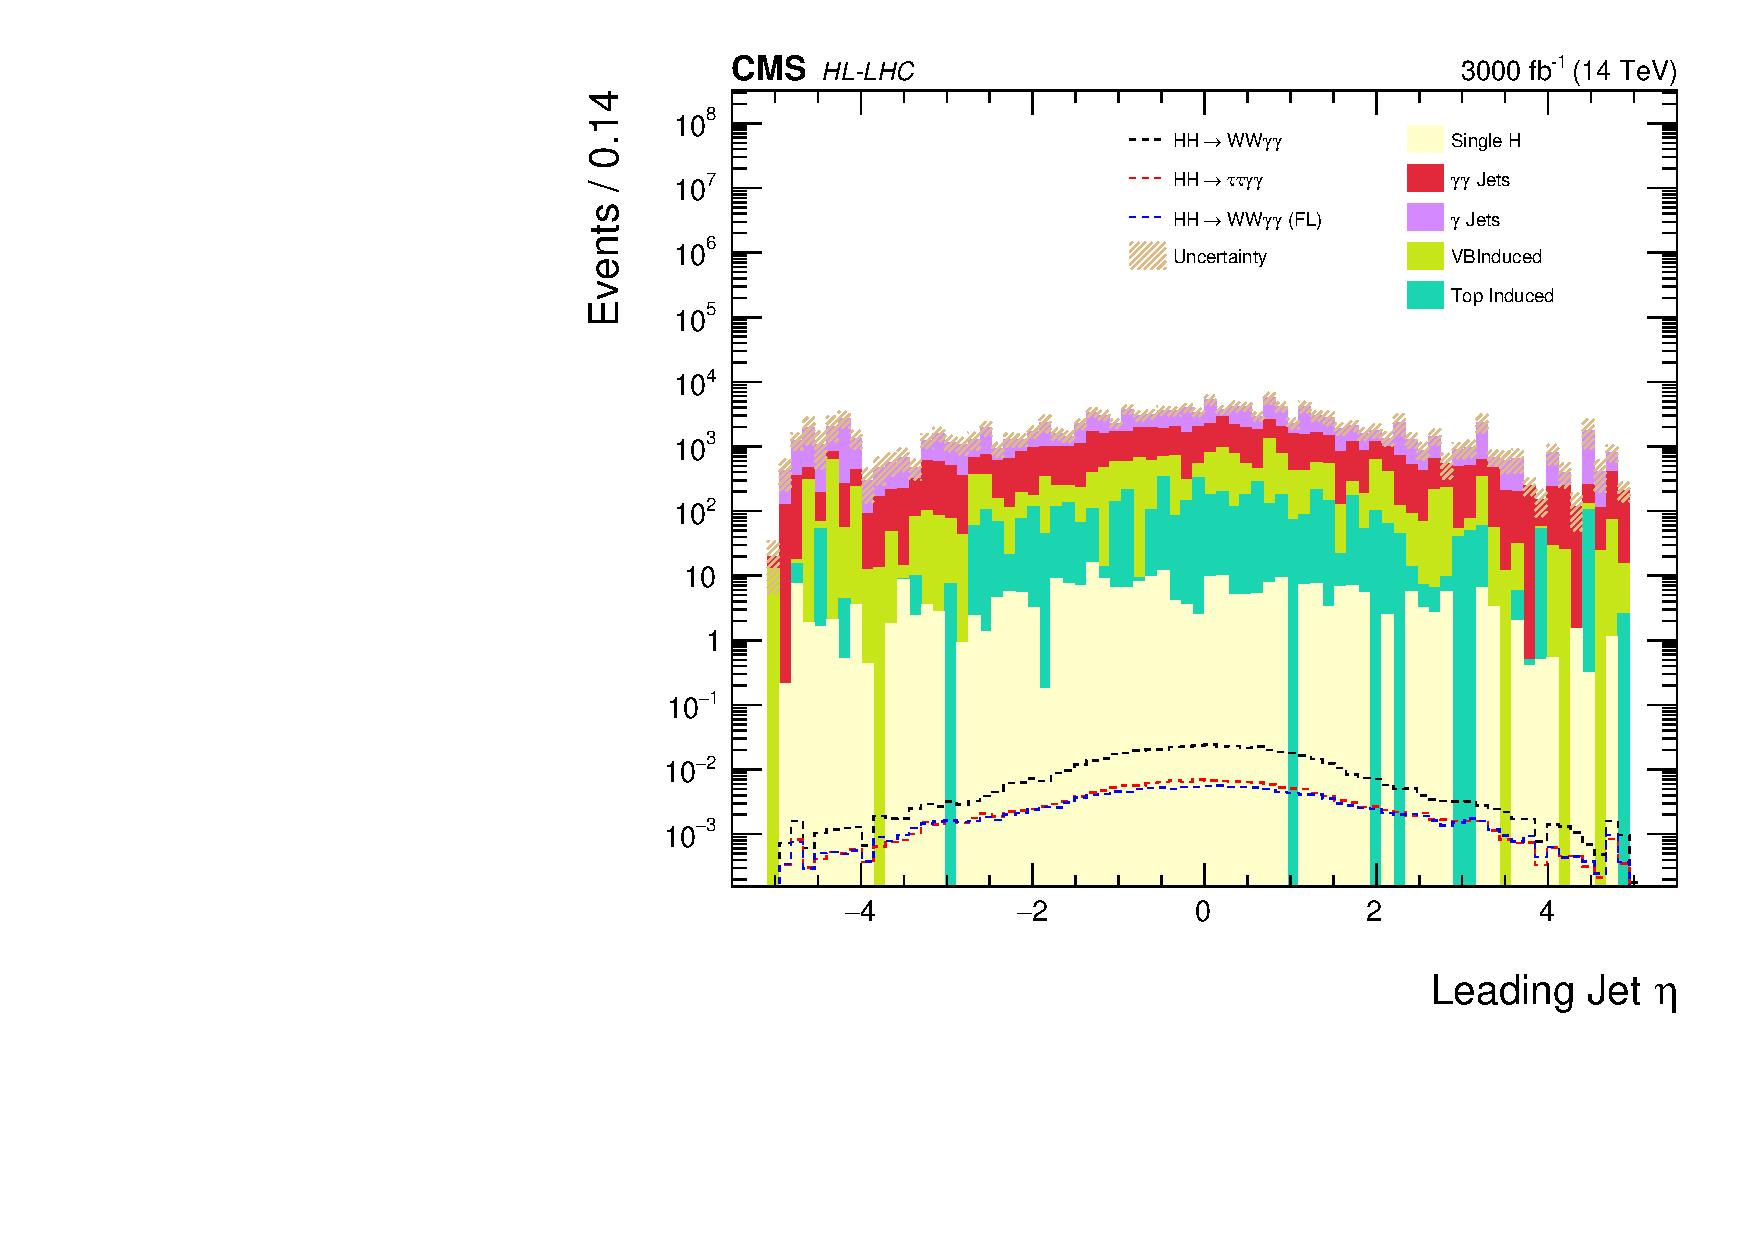
\includegraphics[width=\textwidth]{c3_oneJet_Ljeteta_logy.pdf}
        \vspace{-0.5cm}
        \firstsubcaption{Leading jet $\eta$}
    \end{subfigure}
    \vskip\baselineskip
    \begin{subfigure}[b]{0.475\textwidth}   
        \centering 
        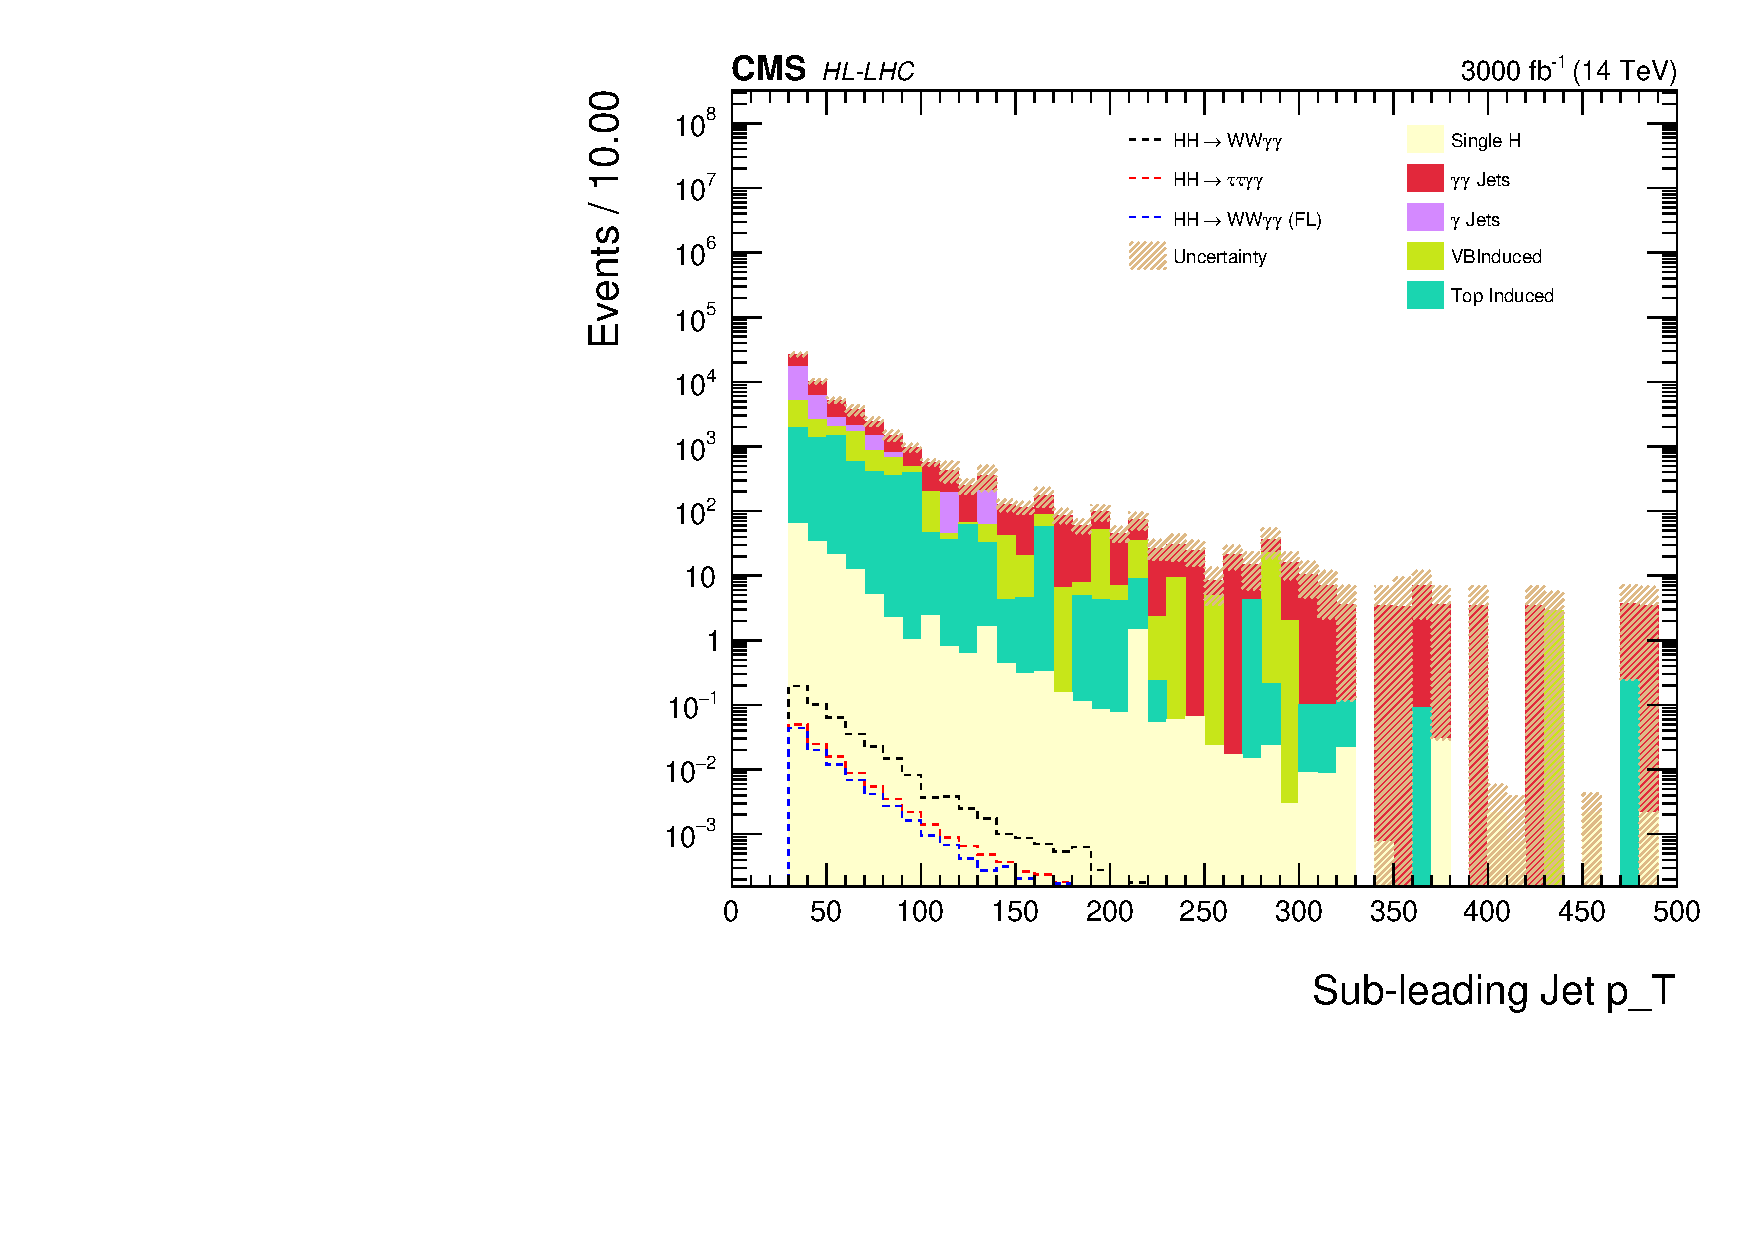
\includegraphics[width=\textwidth]{c3_twoJet_SLjetpt_logy.pdf}
        \vspace{-0.5cm}
        \firstsubcaption{Sub-leading jet \pt}
    \end{subfigure}
    \hfill
    \begin{subfigure}[b]{0.475\textwidth}   
        \centering 
        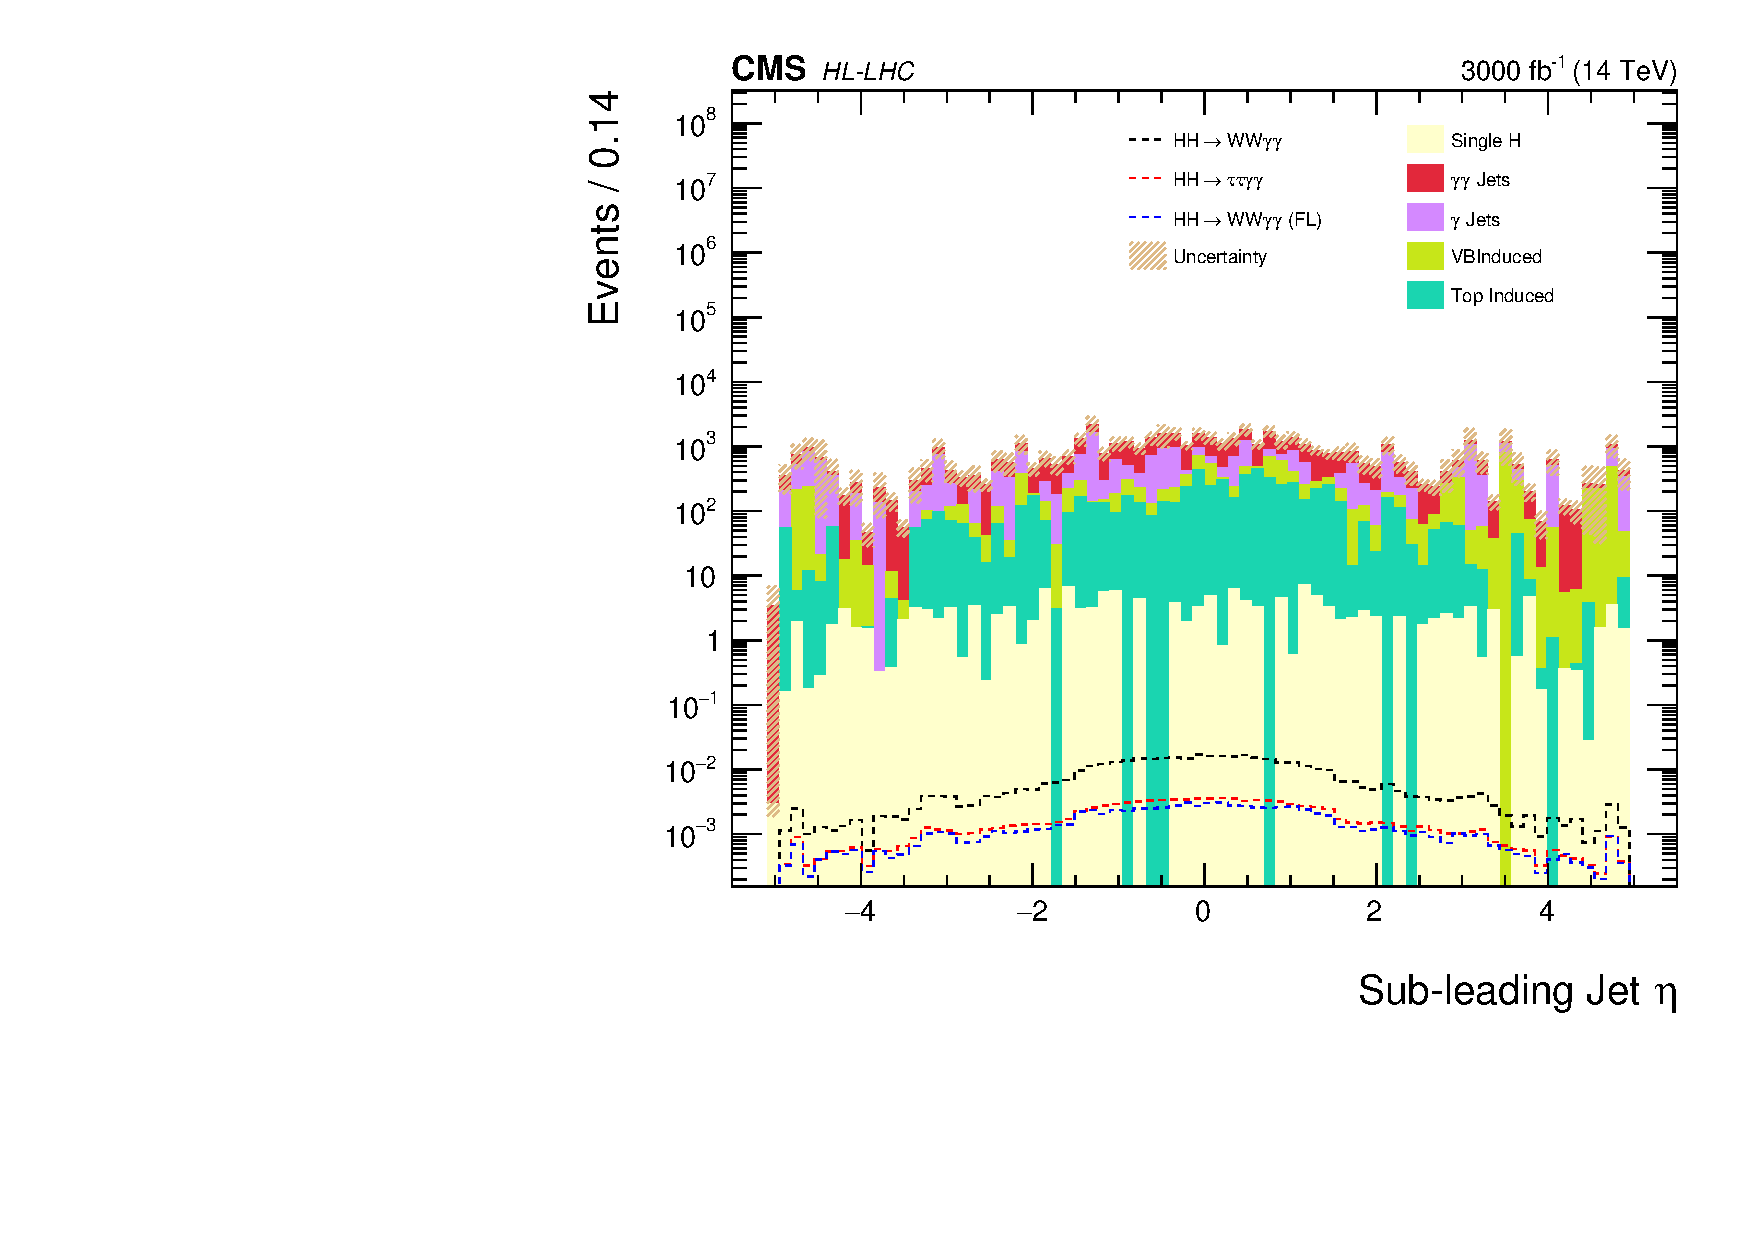
\includegraphics[width=\textwidth]{c3_twoJet_SLjeteta_logy.pdf}
        \vspace{-0.5cm}
        \firstsubcaption{Sub-leading jet $\eta$}   
    \end{subfigure}
    \caption{\small DNN input distributions for the 1$\tau$ channel of $HH\rightarrow{\tau\tau\gamma\gamma}$ (continued).}
\end{figure*}

\begin{figure*}[h!]
    \centering
    \begin{subfigure}[b]{0.475\textwidth}
        \centering
        \includegraphics[width=\textwidth]{c3_met_logy.pdf}
        \vspace{-0.5cm}
        \firstsubcaption{$E_T^{miss}$}
    \end{subfigure}
    \vskip\baselineskip
    \begin{subfigure}[b]{0.475\textwidth}  
        \centering 
        \includegraphics[width=\textwidth]{roc-tau-odd.png}
        \vspace{-0.5cm}
        \firstsubcaption{Odd ROC curve}
    \end{subfigure}
    \hfill
    \begin{subfigure}[b]{0.475\textwidth}   
        \centering 
        \includegraphics[width=\textwidth]{roc-tau-even.png}
        \vspace{-0.5cm}
        \firstsubcaption{Even ROC curve}
    \end{subfigure}
    \vskip\baselineskip
    \begin{subfigure}[b]{0.475\textwidth}   
        \centering 
        \includegraphics[width=\textwidth]{onetau-odd-weights.png}
        \vspace{-0.5cm}
        \firstsubcaption{Odd training weight}
    \end{subfigure}
    \hfill
    \begin{subfigure}[b]{0.475\textwidth}   
        \centering 
        \includegraphics[width=\textwidth]{onetau-even-weights.png}
        \vspace{-0.5cm}
        \firstsubcaption{Even training weight}
    \end{subfigure}
    \caption{\small DNN input distributions for the 1$\tau$ channel of $HH\rightarrow{\tau\tau\gamma\gamma}$ (continued) (a), corresponding ROC curves (b,c) and DNN evaluation on odd (d) and even (e) data.}
\end{figure*}

\begin{landscape}
\begin{table}
\centering
\caption{Cut-flow report showing number of events, before selections, in the single $\tau$ final state and in its categories. Percentages in brackets show the total selection efficiency.}
\begin{tabular}{ |l|c|c|c|c| }
    \hline
    Samples                                & No Selection                   & Single $\tau$        & DNN Cat. 1        & DNN Cat. 2       \\
    \hline
           $HH \rightarrow WW\gamma\gamma$ &  $4.69e+01$  &   $1.82e+00$ (3.879\%) &  $7.97e-01$ (1.699\%) &  $8.60e-01$ (1.833\%) \\
      $HH \rightarrow WW\gamma\gamma (FL)$ &  $1.12e+01$  &   $4.98e-01$ (4.459\%) &  $1.91e-01$ (1.710\%) &  $2.57e-01$ (2.304\%) \\
     $HH \rightarrow \tau\tau\gamma\gamma$ &  $3.13e+00$  &  $5.24e-01$ (16.734\%) &  $2.32e-01$ (7.410\%) &  $2.34e-01$ (7.457\%) \\
                           \textbf{Signal} &  $1.10e+02$  &   $3.19e+00$ (2.908\%) &  $1.44e+00$ (1.310\%) &  $1.43e+00$ (1.303\%) \\
            $GGH \rightarrow \gamma\gamma$ &  $3.44e+05$  &   $6.34e+02$ (0.184\%) &  $1.53e+02$ (0.044\%) &  $8.34e+00$ (0.002\%) \\
           $VBFH \rightarrow \gamma\gamma$ &  $2.85e+04$  &   $7.20e+01$ (0.252\%) &  $3.47e+01$ (0.122\%) &  $3.28e+00$ (0.012\%) \\
            $ttH \rightarrow \gamma\gamma$ &  $4.18e+03$  &   $1.36e+02$ (3.250\%) &  $4.68e+01$ (1.120\%) &  $6.89e+00$ (0.165\%) \\
             $VH \rightarrow \gamma\gamma$ &  $1.63e+04$  &   $1.72e+02$ (1.050\%) &  $6.92e+01$ (0.424\%) &  $2.81e+01$ (0.172\%) \\
                                     $THQ$ &  $6.16e+02$  &   $1.35e+01$ (2.198\%) &  $6.20e+00$ (1.007\%) &  $1.97e+00$ (0.319\%) \\
              $\gamma\gamma + jets 80-Inf$ &  $2.96e+08$  &   $1.42e+05$ (0.048\%) &  $3.58e+04$ (0.012\%) &  $1.82e+03$ (0.001\%) \\
               $\gamma\gamma + jets 40-80$ &  $9.98e+08$  &   $1.99e+03$ (0.000\%) &  $3.46e+02$ (0.000\%) &  $2.82e+01$ (0.000\%) \\
                                  $G+jets$ &  $2.99e+09$  &   $2.10e+05$ (0.007\%) &  $3.33e+04$ (0.001\%) &  $1.49e+03$ (0.000\%) \\
                         $G+jets 20-40GeV$ &  $7.83e+08$  &   $1.12e+04$ (0.001\%) &  $1.64e+02$ (0.000\%) &  $0.00e+00$ (0.000\%) \\
                           $G+jets 20-Inf$ &  $1.17e+10$  &   $4.16e+04$ (0.000\%) &  $1.17e+03$ (0.000\%) &  $0.00e+00$ (0.000\%) \\
                 $W1Jets \rightarrow L\nu$ &  $3.11e+10$  &   $8.04e+03$ (0.000\%) &  $8.04e+02$ (0.000\%) &  $0.00e+00$ (0.000\%) \\
                 $W2Jets \rightarrow L\nu$ &  $8.90e+09$  &   $5.56e+03$ (0.000\%) &  $4.12e+02$ (0.000\%) &  $2.06e+02$ (0.000\%) \\
                 $W3Jets \rightarrow L\nu$ &  $3.80e+09$  &   $6.04e+03$ (0.000\%) &  $1.34e+03$ (0.000\%) &  $6.72e+02$ (0.000\%) \\
                                    $WGJJ$ &  $1.81e+07$  &   $2.00e+03$ (0.011\%) &  $7.63e+02$ (0.004\%) &  $1.71e+02$ (0.001\%) \\
                                 $WGGJets$ &  $5.65e+06$  &   $1.81e+03$ (0.032\%) &  $5.76e+02$ (0.010\%) &  $7.42e+01$ (0.001\%) \\
                                  $DYJets$ &  $1.71e+10$  &   $2.14e+04$ (0.000\%) &  $2.67e+03$ (0.000\%) &  $4.46e+02$ (0.000\%) \\
                                      $ZG$ &  $4.36e+08$  &   $1.52e+04$ (0.003\%) &  $3.76e+03$ (0.001\%) &  $2.63e+02$ (0.000\%) \\
    \hline
\end{tabular}
\label{singletau-cutflow}
\end{table}
\end{landscape}

\begin{landscape}
\begin{table}
\centering
\caption{Cut-flow report showing number of events, before selections, in the single $\tau$ final state and in its categories (cont'd).}
\begin{tabular}{ |l|c|c|c|c| }
    \hline
    Samples                                & No Selection                   & Single $\tau$        & DNN Cat. 1        & DNN Cat. 2       \\
    \hline
    $WW(inclusive)$ &  $2.11e+08$  &   $5.65e+02$ (0.000\%) &  $1.66e+02$ (0.000\%) &  $2.34e+01$ (0.000\%) \\
                    $t\bar{t} (inclusive)$ &  $2.59e+09$  &   $2.29e+04$ (0.001\%) &  $5.51e+03$ (0.000\%) &  $4.20e+02$ (0.000\%) \\
                                 $ttGJets$ &  $1.37e+07$  &   $4.50e+03$ (0.033\%) &  $1.30e+03$ (0.009\%) &  $8.62e+01$ (0.001\%) \\
                                    $ttGG$ &  $5.59e+04$  &   $2.47e+02$ (0.441\%) &  $6.72e+01$ (0.120\%) &  $7.81e+00$ (0.014\%) \\
                                     $ttW$ &  $6.76e+05$  &   $2.85e+01$ (0.004\%) &  $6.31e+00$ (0.001\%) &  $2.52e-01$ (0.000\%) \\
                       \textbf{Background} &  $8.10e+10$  &   $4.96e+05$ (0.001\%) &  $8.85e+04$ (0.000\%) &  $5.76e+03$ (0.000\%) \\
    \hline
\end{tabular}
\end{table}
\end{landscape}

%%%%%%%%%%%%%%%%%%%%%%%%%%%%%%%%%%%%%%%%%%%%%%%%%%%%
%%%%%%%%%%%%%%%%%%%%%%%%%%%%%%%%%%%%%%%%%%%%%%%%%%%%
%%%%%%%%%%%%%%%%%%%%%%%%%%%%%%%%%%%%%%%%%%%%%%%%%%%%

\section*{APPENDIX A.7}
\vglue6pt

\begin{table}
\centering
\caption{Cut-flow report showing number of events, before selections and in the double $\tau$ final state of $HH\rightarrow{\tau\tau\gamma\gamma}$.}
\begin{tabular}{ |l|c|c| }
    \hline
    Samples                                & noSel                   & Two Taus              \\
    \hline
           $HH \rightarrow WW\gamma\gamma$ &  $4.69e+01$  &  $8.29e-02$ (0.177\%) \\
      $HH \rightarrow WW\gamma\gamma (FL)$ &  $1.12e+01$  &  $2.48e-02$ (0.222\%) \\
     $HH \rightarrow \tau\tau\gamma\gamma$ &  $3.13e+00$  &  $1.10e-01$ (3.495\%) \\
                           \textbf{Signal} &  $1.10e+02$  &  $2.22e-01$ (0.202\%) \\
            $GGH \rightarrow \gamma\gamma$ &  $3.44e+05$  &  $1.39e+00$ (0.000\%) \\
           $VBFH \rightarrow \gamma\gamma$ &  $2.85e+04$  &  $1.08e-01$ (0.000\%) \\
            $ttH \rightarrow \gamma\gamma$ &  $4.18e+03$  &  $7.17e+00$ (0.171\%) \\
             $VH \rightarrow \gamma\gamma$ &  $1.63e+04$  &  $4.29e+00$ (0.026\%) \\
                                     $THQ$ &  $6.16e+02$  &  $3.41e-01$ (0.055\%) \\
              $\gamma\gamma + jets 80-Inf$ &  $2.96e+08$  &  $5.14e+02$ (0.000\%) \\
               $\gamma\gamma + jets 40-80$ &  $9.98e+08$  &  $7.06e+00$ (0.000\%) \\
                                  $G+jets$ &  $2.99e+09$  &  $0.00e+00$ (0.000\%) \\
                         $G+jets 20-40GeV$ &  $7.83e+08$  &  $0.00e+00$ (0.000\%) \\
                           $G+jets 20-Inf$ &  $1.17e+10$  &  $0.00e+00$ (0.000\%) \\
                 $W1Jets \rightarrow L\nu$ &  $3.11e+10$  &  $0.00e+00$ (0.000\%) \\
                 $W2Jets \rightarrow L\nu$ &  $8.90e+09$  &  $0.00e+00$ (0.000\%) \\
                 $W3Jets \rightarrow L\nu$ &  $3.80e+09$  &  $0.00e+00$ (0.000\%) \\
                                    $WGJJ$ &  $1.81e+07$  &  $1.00e+01$ (0.000\%) \\
                                 $WGGJets$ &  $5.65e+06$  &  $8.56e+00$ (0.000\%) \\
                                  $DYJets$ &  $1.71e+10$  &  $2.23e+02$ (0.000\%) \\
                                      $ZG$ &  $4.36e+08$  &  $7.33e+02$ (0.000\%) \\
                           $WW(inclusive)$ &  $2.11e+08$  &  $1.49e+01$ (0.000\%) \\
                    $t\bar{t} (inclusive)$ &  $2.59e+09$  &  $1.05e+03$ (0.000\%) \\
                                 $ttGJets$ &  $1.37e+07$  &  $1.45e+02$ (0.001\%) \\
                                    $ttGG$ &  $5.59e+04$  &  $9.98e+00$ (0.018\%) \\
                                     $ttW$ &  $6.76e+05$  &  $2.52e+00$ (0.000\%) \\
                       \textbf{Background} &  $8.10e+10$  &  $2.73e+03$ (0.000\%) \\
    \hline
\end{tabular}
\label{cutflow-doubletau}
\end{table}

%%%%%%%%%%%%%%%%%%%%%%%%%%%%%%%%%%%%%%%%%%%%%%%%%%%%
%%%%%%%%%%%%%%%%%%%%%%%%%%%%%%%%%%%%%%%%%%%%%%%%%%%%
%%%%%%%%%%%%%%%%%%%%%%%%%%%%%%%%%%%%%%%%%%%%%%%%%%%%

\section*{APPENDIX A.8}
\vglue6pt

\begin{figure*}[h!]
    \centering
    \begin{subfigure}[b]{0.475\textwidth}
        \centering
        \includegraphics[width=\textwidth]{Inv_mass_gghasOneL_DNN_HL_FIT.pdf}
        \vspace{-0.5cm}
        \firstsubcaption{Cat. 1}
    \end{subfigure}
    \vskip\baselineskip
    \begin{subfigure}[b]{0.475\textwidth}  
        \centering 
        \includegraphics[width=\textwidth]{Inv_mass_gghasOneL_DNN_2_HL_FIT.pdf}
        \vspace{-0.5cm}
        \firstsubcaption{Cat. 2}
    \end{subfigure}
    \hfill
    \begin{subfigure}[b]{0.475\textwidth}   
        \centering 
        \includegraphics[width=\textwidth]{Inv_mass_gghasOneL_DNN_3_HL_FIT.pdf}
        \vspace{-0.5cm}
        \firstsubcaption{Cat. 3}
    \end{subfigure}
    \vskip\baselineskip
    \begin{subfigure}[b]{0.475\textwidth}   
        \centering 
        \includegraphics[width=\textwidth]{Inv_mass_gghasOneL_HL_FIT.pdf}
        \vspace{-0.5cm}
        \firstsubcaption{Semi-leptonic}
    \end{subfigure}
    \hfill
    \begin{subfigure}[b]{0.475\textwidth}   
        \centering 
        \includegraphics[width=\textwidth]{Inv_mass_gghasTwoL_HL_FIT.pdf}
        \vspace{-0.5cm}
        \firstsubcaption{Fully-leptonic}
    \end{subfigure}
    \caption{\small Fitted distributions of semi-leptonic channel (a,b,c) and fully-leptonic (d,e) channel of \wwgg.}
\label{allfits}
\end{figure*}

\begin{figure*}[h!]
    \centering
    \begin{subfigure}[b]{0.475\textwidth}
        \centering
        \includegraphics[width=\textwidth]{Mgg_c3_HL_FIT.pdf}
        \vspace{-0.5cm}
        \firstsubcaption{Single $\tau$}
    \end{subfigure}
    \hfill
    \begin{subfigure}[b]{0.475\textwidth}  
        \centering 
        \includegraphics[width=\textwidth]{Mgg_c3_DNN_HL_FIT.pdf}
        \vspace{-0.5cm}
        \firstsubcaption{Single $\tau$ Cat. 1}
    \end{subfigure}
    \vskip\baselineskip
    \begin{subfigure}[b]{0.475\textwidth}   
        \centering 
        \includegraphics[width=\textwidth]{Mgg_c4_Zveto_HL_FIT.pdf}
        \vspace{-0.5cm}
        \firstsubcaption{Double $\tau$}
    \end{subfigure}
    \caption{\small Fitted distributions of single $\tau$ (a,b) and double $\tau$ channels of \ttgg.}
\label{allfits2}
\end{figure*}